% !TEX program = xelatex
\documentclass[UTF8,fontset=fandol,a4paper,11pt]{ctexart}
\usepackage[margin=21mm,top=23mm,bottom=22mm,headheight=16pt]{geometry}
\usepackage{amsmath,amssymb,mathtools,bm}
\usepackage{tikz}
\usetikzlibrary{arrows.meta,calc,angles,quotes,patterns}
\usepackage{xcolor,booktabs,array,longtable,enumitem,fancyhdr,needspace}
\usepackage[unicode,hidelinks]{hyperref}
\definecolor{ink}{HTML}{24343C}
\definecolor{accent}{HTML}{166A70}
\definecolor{muted}{HTML}{65747A}
\definecolor{rulegray}{HTML}{D4DDE0}
\definecolor{warm}{HTML}{966037}
\color{ink}
\setlength{\parindent}{2em}
\setlength{\parskip}{4pt}
\linespread{1.12}
\AtBeginDocument{\setlength{\abovedisplayskip}{6pt plus 2pt minus 1pt}
\setlength{\belowdisplayskip}{6pt plus 2pt minus 1pt}
\setlength{\abovedisplayshortskip}{0pt plus 1pt}
\setlength{\belowdisplayshortskip}{4pt plus 1pt}}
\setlist[enumerate]{label=(\arabic*),leftmargin=2.3em,itemsep=3pt,topsep=4pt}
\setlist[itemize]{leftmargin=2em,itemsep=2pt,topsep=4pt}
\allowdisplaybreaks[1]
\setlength{\emergencystretch}{2em}
\setcounter{secnumdepth}{0}
\providecommand{\tightlist}{\setlength{\itemsep}{0pt}\setlength{\parskip}{0pt}}
\ctexset{section={format=\Large\bfseries\color{accent},beforeskip=10pt,afterskip=9pt},
subsection={format=\normalsize\bfseries\color{accent},beforeskip=10pt,afterskip=4pt},
subsubsection={format=\normalsize\bfseries,beforeskip=8pt,afterskip=3pt}}
\pagestyle{fancy}
\fancyhf{}
\fancyhead[L]{\small\color{muted}物理学难题集萃}
% 页眉仅保留书名；版本名称只在封面显示。
\fancyfoot[L]{\small\color{muted}\chapterlabel}
\fancyfoot[R]{\small\thepage}
\renewcommand{\headrulewidth}{0.4pt}
\renewcommand{\footrulewidth}{0pt}
\newcommand{\dd}{\mathop{}\!\mathrm{d}}
\newcommand{\vect}[1]{\bm{#1}}
\newcommand{\tagline}[1]{\noindent{\small\color{muted}#1}\par}
\newcommand{\result}[1]{\begin{equation*}\boxed{#1}\end{equation*}}
\newcommand{\figcaption}[1]{\par\vspace{2pt}{\small\color{muted}#1}\par}
\newcommand{\teach}[2]{\Needspace{4\baselineskip}\subsection*{讲解要点与追问}#1\par\smallskip\noindent\textbf{追问：}#2\par}
\newcommand{\workarea}{\par\vspace{7mm}\noindent{\small\color{muted}作答区}\par\vspace{4mm}
\noindent\textcolor{rulegray}{\rule{\linewidth}{0.3pt}}\par\vspace{16mm}
\noindent\textcolor{rulegray}{\rule{\linewidth}{0.3pt}}\par\vspace{16mm}
\noindent\textcolor{rulegray}{\rule{\linewidth}{0.3pt}}\par\vspace{16mm}
\noindent\textcolor{rulegray}{\rule{\linewidth}{0.3pt}}}
\tikzset{axis/.style={-{Stealth[length=2mm]},thin,color=muted},
motion/.style={-{Stealth[length=2.3mm]},thick,color=accent},
force/.style={-{Stealth[length=2.3mm]},thick,color=warm},
traj/.style={thick,color=accent},guide/.style={dashed,thin,color=muted},
object/.style={thick,color=ink},every node/.style={font=\small}}\widowpenalty=10000\clubpenalty=10000\displaywidowpenalty=10000\newcommand{\chapterlabel}{热学试题（二）}







\hypersetup{pdftitle={热学试题（二）·教师版},pdfauthor={}}

\begin{document}\pdfbookmark[0]{热学试题（二）}{cover}

\thispagestyle{empty}\vspace*{22mm}

\noindent{\Huge\bfseries 物理学难题集萃}\par\vspace{12mm}

\noindent{\LARGE 热学试题（二）}\par\vspace{12mm}

\noindent{\Large\color{accent}教师版}\par\vspace{9mm}

\noindent\textcolor{accent}{\rule{\linewidth}{1pt}}\par\vspace{9mm}

\noindent 第1--5题\par\vfill\clearpage

\pdfbookmark[1]{题目目录}{contents}\section*{题目目录}

\begin{longtable}{@{}r p{113mm} r@{}}\toprule 题号 & 题目 & 页码\\\midrule

\hyperref[q:1]{1} & \hyperref[q:1]{热容量阶跃下的矩形循环} & \pageref{q:1} \\

\hyperref[q:2]{2} & \hyperref[q:2]{有限热源的最大作功与相变卡诺循环} & \pageref{q:2} \\

\hyperref[q:3]{3} & \hyperref[q:3]{从活塞与分子碰撞导出绝热方程} & \pageref{q:3} \\

\hyperref[q:4]{4} & \hyperref[q:4]{导热稳态、分子扩散与撤热源后的平衡} & \pageref{q:4} \\

\hyperref[q:5]{5} & \hyperref[q:5]{光子气体的压强、绝热关系与辐射能流} & \pageref{q:5} \\

\bottomrule\end{longtable}

\clearpage

\pdfbookmark[2]{第 1 题 热容量阶跃下的矩形循环}{q1}

\section*{第 1 题\quad 热容量阶跃下的矩形循环}\label{q:1}


$\nu$ mol理想气体的定体摩尔热容量为
\[
C_V(T)=
\begin{cases}
\alpha R,&T<2T_0,\\
\alpha\beta R,&T>2T_0,
\end{cases}
\qquad \alpha>1,\quad\beta>1.
\]
气体内能由给定热容量连续积分确定，取$U(0)=0$。气体经历图热试2.1所示的顺时针矩形循环$A\to B\to C\to D\to A$，其中$AB,CD$等体，$BC,DA$等压，已知$T_A=T_0,T_B=2T_0,T_C=3T_0$。
\begin{enumerate}
\item 求$T_D$，画$U$--$T$关系，并在图中标出四态及$CD$上$T=2T_0$的状态$E$。
\item 求循环效率；说明热容量的阶跃是否足以引入定温吸放热。
\end{enumerate}


\begin{center}\begin{minipage}{.98\linewidth}\centering
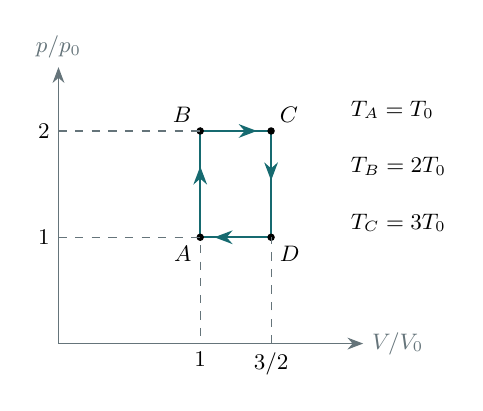
\begin{tikzpicture}[scale=.9,transform shape]

\draw[axis] (0,0)--(4.3,0) node[right] {$V/V_0$};
\draw[axis] (0,0)--(0,3.9) node[above] {$p/p_0$};
\draw[traj] (2,1.5)--(2,3)--(3,3)--(3,1.5)--cycle;
\draw[motion] (2,1.9)--(2,2.5);
\draw[motion] (2.2,3)--(2.8,3);
\draw[motion] (3,2.7)--(3,2.3);
\draw[motion] (2.8,1.5)--(2.2,1.5);
\foreach \x/\y/\lab/\pos in {2/1.5/A/below left,2/3/B/above left,3/3/C/above right,3/1.5/D/below right}{
\fill (\x,\y) circle (1.5pt) node[\pos] {$\lab$};}
\node[below] at (2,0) {$1$};\node[below] at (3,0) {$3/2$};
\node[left] at (0,1.5) {$1$};\node[left] at (0,3) {$2$};
\draw[guide] (0,1.5)--(2,1.5)--(2,0);
\draw[guide] (0,3)--(2,3);\draw[guide] (3,0)--(3,1.5);

\node[right] at (4,3.3) {$T_A=T_0$};
\node[right] at (4,2.5) {$T_B=2T_0$};
\node[right] at (4,1.7) {$T_C=3T_0$};

\end{tikzpicture}
\figcaption{图热试2.1\quad 顺时针矩形循环；体积与压强坐标按初态归一化。}
\end{minipage}\end{center}

\Needspace{8\baselineskip}

\pdfbookmark[3]{题型定位}{q1-h0}

\subsection*{题型定位}

热容量随温度改变时，以$\mathrm dU=\nu C_V\mathrm dT$为起点做分段积分；矩形循环的各态温度和作功则由状态方程与几何路径确定。将这两部分结合，逐段计算热量，再由正吸热量与净功求效率。热容量有限阶跃改变内能曲线的斜率，额外潜热由独立的相变条件指定。

\Needspace{8\baselineskip}

\pdfbookmark[3]{知识点}{q1-h1}

\subsection*{知识点}

理想气体状态方程$pV=\nu RT$把矩形的四顶点与温度联系起来；热量满足$Q=\Delta U+W$，等体段$W=0$，等压段$W=p\Delta V$。给定摩尔热容量后，内能由温度积分加一个全局基准确定，分段表达式在连接温度匹配。热容量阶跃有限时积分连续，潜热则对应另给的能量跃变。熵的积分还包含$\nu R\ln V$，因此$U$、$T$相同的两态仍可具有不同体积和熵。

\Needspace{8\baselineskip}

\pdfbookmark[3]{物理图像}{q1-h2}

\subsection*{物理图像}

题图的矩形顺时针闭合，净功是面积$p_0V_0/2$。解图热试2.1A把状态投影到$U$—$T$平面：$B,E$重合，折线在温度$2T_0$处改变斜率。它们在题图中分别位于左、右两条等体线上，体积不同。图B把冷却段在$E$处分开；图C固定矩形与$\alpha$，显示高温热容量增大时吸热增加、效率降低。

\Needspace{8\baselineskip}

\pdfbookmark[3]{解题入口}{q1-h3}

\subsection*{解题入口}

先从$A$给出的$p_0,V_0,T_0$依次得到$B,C,D$的压强和体积，确定$T_D$与$E$的位置。随后把$C_V(T)$从零温积分，先算到$2T_0$，高温段在这个内能值上继续累加。得到四态内能后，按图B的路径分别列$\Delta U$与$W$。吸热段的温度沿$AB,BC$上升，放热段沿$CD,DA$下降，各段热量由对应的内能变化和机械功相加确定正负。

\Needspace{8\baselineskip}

\pdfbookmark[3]{标准解法}{q1-h4}

\subsection*{标准解法}


图热试2.1中取$A$态压强、体积为$p_0,V_0$，满足$p_0V_0=\nu RT_0$。由$AB$等体且$T_B=2T_0$，得$p_B=2p_0$；$BC$等压且$T_C=3T_0$，得$V_C=3V_0/2$。于是
\[
D:\quad p_D=p_0,\quad V_D=\frac32V_0,
\qquad
\boxed{T_D=\frac32T_0}.
\]
在$CD$上$V=3V_0/2$不变，因此$T_E=2T_0$处$p_E=4p_0/3$。

$E$与$B$有同一温度，但等体线不同：$E$在右侧的$V=3V_0/2$上，$B$在左侧的$V=V_0$上。矩形路径的各态依次为$(p/p_0,V/V_0)=(1,1),(2,1),(2,3/2),(1,3/2)$，对应温度依次为$1,2,3,3/2$倍$T_0$。由热容量定义$\mathrm dU=\nu C_V(T)\,\mathrm dT$，应从零温基准分段积分：
\[
U(T)=
\begin{cases}
\alpha\nu RT,&0\le T\le2T_0,\\[2pt]
2\alpha\nu RT_0+\alpha\beta\nu R(T-2T_0),&T\ge2T_0.
\end{cases}
\]
具体地，低温段从$U(0)=0$积到$U(2T_0)=\nu\int_0^{2T_0}\alpha R\mathrm dT$。高温段再从这个值继续累积$\nu\int_{2T_0}^T\alpha\beta R\mathrm dT$，于是斜率变为$\alpha\beta\nu R$，连接温度的内能值仍由前段确定。两段在$2T_0$处都等于$2\alpha\nu RT_0$，所以内能连续，只有斜率发生改变。高温段保留低温积分累积的$2\alpha\nu RT_0$，并从$2T_0$开始按新热容量继续积分，所以两段的积分常数彼此匹配。
\begin{center}\begin{minipage}{.98\linewidth}\centering
\begin{tikzpicture}[scale=.8,transform shape]
\draw[axis] (0,0)--(10.7,0) node[right] {$T/T_0$};
\draw[axis] (0,0)--(0,3.2) node[above] {$U/(\alpha\nu RT_0)$};
\node[above] at (5,3.5) {$\beta=2$示例：内能在温度2处连续};
\draw[traj] plot coordinates {(0.000000000,0.000000000) (0.064000000,0.014000000) (0.128000000,0.028000000) (0.192000000,0.042000000) (0.256000000,0.056000000) (0.320000000,0.070000000) (0.384000000,0.084000000) (0.448000000,0.098000000) (0.512000000,0.112000000) (0.576000000,0.126000000) (0.640000000,0.140000000) (0.704000000,0.154000000) (0.768000000,0.168000000) (0.832000000,0.182000000) (0.896000000,0.196000000) (0.960000000,0.210000000) (1.024000000,0.224000000) (1.088000000,0.238000000) (1.152000000,0.252000000) (1.216000000,0.266000000) (1.280000000,0.280000000) (1.344000000,0.294000000) (1.408000000,0.308000000) (1.472000000,0.322000000) (1.536000000,0.336000000) (1.600000000,0.350000000) (1.664000000,0.364000000) (1.728000000,0.378000000) (1.792000000,0.392000000) (1.856000000,0.406000000) (1.920000000,0.420000000) (1.984000000,0.434000000) (2.048000000,0.448000000) (2.112000000,0.462000000) (2.176000000,0.476000000) (2.240000000,0.490000000) (2.304000000,0.504000000) (2.368000000,0.518000000) (2.432000000,0.532000000) (2.496000000,0.546000000) (2.560000000,0.560000000) (2.624000000,0.574000000) (2.688000000,0.588000000) (2.752000000,0.602000000) (2.816000000,0.616000000) (2.880000000,0.630000000) (2.944000000,0.644000000) (3.008000000,0.658000000) (3.072000000,0.672000000) (3.136000000,0.686000000) (3.200000000,0.700000000) (3.264000000,0.714000000) (3.328000000,0.728000000) (3.392000000,0.742000000) (3.456000000,0.756000000) (3.520000000,0.770000000) (3.584000000,0.784000000) (3.648000000,0.798000000) (3.712000000,0.812000000) (3.776000000,0.826000000) (3.840000000,0.840000000) (3.904000000,0.854000000) (3.968000000,0.868000000) (4.032000000,0.882000000) (4.096000000,0.896000000) (4.160000000,0.910000000) (4.224000000,0.924000000) (4.288000000,0.938000000) (4.352000000,0.952000000) (4.416000000,0.966000000) (4.480000000,0.980000000) (4.544000000,0.994000000) (4.608000000,1.008000000) (4.672000000,1.022000000) (4.736000000,1.036000000) (4.800000000,1.050000000) (4.864000000,1.064000000) (4.928000000,1.078000000) (4.992000000,1.092000000) (5.056000000,1.106000000) (5.120000000,1.120000000) (5.184000000,1.134000000) (5.248000000,1.148000000) (5.312000000,1.162000000) (5.376000000,1.176000000) (5.440000000,1.190000000) (5.504000000,1.204000000) (5.568000000,1.218000000) (5.632000000,1.232000000) (5.696000000,1.246000000) (5.760000000,1.260000000) (5.824000000,1.274000000) (5.888000000,1.288000000) (5.952000000,1.302000000) (6.016000000,1.316000000) (6.080000000,1.330000000) (6.144000000,1.344000000) (6.208000000,1.358000000) (6.272000000,1.372000000) (6.336000000,1.386000000) (6.400000000,1.400000000) (6.464000000,1.428000000) (6.528000000,1.456000000) (6.592000000,1.484000000) (6.656000000,1.512000000) (6.720000000,1.540000000) (6.784000000,1.568000000) (6.848000000,1.596000000) (6.912000000,1.624000000) (6.976000000,1.652000000) (7.040000000,1.680000000) (7.104000000,1.708000000) (7.168000000,1.736000000) (7.232000000,1.764000000) (7.296000000,1.792000000) (7.360000000,1.820000000) (7.424000000,1.848000000) (7.488000000,1.876000000) (7.552000000,1.904000000) (7.616000000,1.932000000) (7.680000000,1.960000000) (7.744000000,1.988000000) (7.808000000,2.016000000) (7.872000000,2.044000000) (7.936000000,2.072000000) (8.000000000,2.100000000) (8.064000000,2.128000000) (8.128000000,2.156000000) (8.192000000,2.184000000) (8.256000000,2.212000000) (8.320000000,2.240000000) (8.384000000,2.268000000) (8.448000000,2.296000000) (8.512000000,2.324000000) (8.576000000,2.352000000) (8.640000000,2.380000000) (8.704000000,2.408000000) (8.768000000,2.436000000) (8.832000000,2.464000000) (8.896000000,2.492000000) (8.960000000,2.520000000) (9.024000000,2.548000000) (9.088000000,2.576000000) (9.152000000,2.604000000) (9.216000000,2.632000000) (9.280000000,2.660000000) (9.344000000,2.688000000) (9.408000000,2.716000000) (9.472000000,2.744000000) (9.536000000,2.772000000) (9.600000000,2.800000000)};
\node[below] at (0,-.12) {$0$};
\node[below] at (3.2,-.12) {$1$};
\node[below] at (4.8,-.12) {$3/2$};
\node[below] at (6.4,-.12) {$2$};
\node[below] at (9.6,-.12) {$3$};
\fill (3.2,.7) circle(.04) node[above left] {$A$};\fill (4.8,1.05) circle(.04) node[below right] {$D$};\fill (6.4,1.4) circle(.04) node[above left] {$B,E$};\fill (9.6,2.8) circle(.04) node[above] {$C$};\end{tikzpicture}
\figcaption{解图热试2.1A\quad $\beta=2$示例：内能在温度2处连续}
\end{minipage}\end{center}
解图热试2.1A以$t=T/T_0$、$u=U/(\alpha\nu RT_0)$为坐标，折线为
\[
u=t\quad(t\le2),\qquad u=2+\beta(t-2)\quad(t\ge2).
\]
四态的内能分别为
\[
U_A=\alpha\nu RT_0,\quad U_B=2\alpha\nu RT_0,\quad
U_C=\alpha(\beta+2)\nu RT_0,\quad
U_D=\frac32\alpha\nu RT_0.
\]
$B,E$在$U$--$T$图上重合，但$V_B=V_0$、$V_E=3V_0/2$，在$p$--$V$图上是两个状态；理想气体的内能只由温度确定，体积与压强还由状态方程及所在过程分别确定。

\begin{center}\begin{minipage}{.98\linewidth}\centering
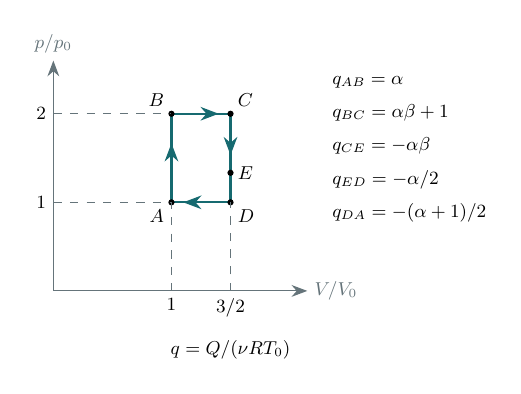
\begin{tikzpicture}[scale=.75,transform shape]

\draw[axis] (0,0)--(4.3,0) node[right] {$V/V_0$};
\draw[axis] (0,0)--(0,3.9) node[above] {$p/p_0$};
\draw[traj] (2,1.5)--(2,3)--(3,3)--(3,1.5)--cycle;
\draw[motion] (2,1.9)--(2,2.5);
\draw[motion] (2.2,3)--(2.8,3);
\draw[motion] (3,2.7)--(3,2.3);
\draw[motion] (2.8,1.5)--(2.2,1.5);
\foreach \x/\y/\lab/\pos in {2/1.5/A/below left,2/3/B/above left,3/3/C/above right,3/1.5/D/below right}{
\fill (\x,\y) circle (1.5pt) node[\pos] {$\lab$};}
\node[below] at (2,0) {$1$};\node[below] at (3,0) {$3/2$};
\node[left] at (0,1.5) {$1$};\node[left] at (0,3) {$2$};
\draw[guide] (0,1.5)--(2,1.5)--(2,0);
\draw[guide] (0,3)--(2,3);\draw[guide] (3,0)--(3,1.5);

\fill (3,2) circle (1.5pt) node[right] {$E$};
\node[align=left,right] at (4.6,2.4) {$q_{AB}=\alpha$\\[5pt]$q_{BC}=\alpha\beta+1$\\[5pt]$q_{CE}=-\alpha\beta$\\[5pt]$q_{ED}=-\alpha/2$\\[5pt]$q_{DA}=-(\alpha+1)/2$};
\node at (3,-1) {$q=Q/(\nu RT_0)$};

\end{tikzpicture}
\figcaption{解图热试2.1B\quad 冷却在E处分段，各段热量之和等于矩形面积功。}
\end{minipage}\end{center}
图A的两段直线以$\beta=2$示例，低温斜率为1，高温斜率为2；一般$\beta$只改变高温段斜率。沿$AB$逐渐升温时，内能图上的点从$A$走向$B$；沿$CD$逐渐降温时，从$C$经与$B$重合的$E$走向$D$。$D$也与$AB$上某状态投影重合，因为它们温度相同；各态在完整$p$—$V$空间中的位置由不同等体线区分。

解图热试2.1B将$CD$的冷却按$E$分开，用各段正确热容量计算。以下以$q=Q/(\nu RT_0)$表示代数热量，吸热为正：
\[
q_{AB}=\alpha,\qquad
q_{BC}=\alpha\beta+1.
\]
其中$BC$有$\Delta U=\alpha\beta\nu RT_0$，还做功$2p_0(V_0/2)=\nu RT_0$。在$CD$上先由$3T_0$降到$2T_0$，再由$2T_0$降到$3T_0/2$，故
\[
q_{CD}=-\alpha\beta-\frac12\alpha,
\qquad
q_{DA}=-\frac12(\alpha+1).
\]
$DA$的内能变化为$-\alpha\nu RT_0/2$，压缩功为$-p_0V_0/2$。冷却的两段分别有$q_{CE}=-\alpha\beta$与$q_{ED}=-\alpha/2$；它们温降分别为$T_0$与$T_0/2$，均为负热量。$AB$与$BC$的代数热量为正，$CD$与$DA$为负，因此正吸热量取前两项之和，正放热量取后两项相反数之和。合计正吸热量、正放热量与净功：
\[
Q_{\rm in}=[\alpha(1+\beta)+1]\nu RT_0,
\]
\[
Q_{\rm out}=\left[\alpha(1+\beta)+\frac12\right]\nu RT_0,
\qquad
W_{\rm cyc}=\frac12\nu RT_0.
\]
净功也等于$p$--$V$矩形面积
\[
(2p_0-p_0)\left(\frac32V_0-V_0\right)
=\frac12p_0V_0,
\]
因此
\[
\boxed{\eta=\frac1{2[\alpha(1+\beta)+1]}}.
\]
\begin{center}\begin{minipage}{.98\linewidth}\centering
\begin{tikzpicture}[scale=.8,transform shape]
\draw[axis] (0,0)--(10.7,0) node[right] {$\beta$};
\draw[axis] (0,0)--(0,3.2) node[above] {$\eta$};
\node[above] at (5,3.5) {$\alpha=2$：矩形功固定，吸热增大};
\draw[traj] plot coordinates {(0.000000000,2.800000000) (0.083333333,2.763157895) (0.166666667,2.727272727) (0.250000000,2.692307692) (0.333333333,2.658227848) (0.416666667,2.625000000) (0.500000000,2.592592593) (0.583333333,2.560975610) (0.666666667,2.530120482) (0.750000000,2.500000000) (0.833333333,2.470588235) (0.916666667,2.441860465) (1.000000000,2.413793103) (1.083333333,2.386363636) (1.166666667,2.359550562) (1.250000000,2.333333333) (1.333333333,2.307692308) (1.416666667,2.282608696) (1.500000000,2.258064516) (1.583333333,2.234042553) (1.666666667,2.210526316) (1.750000000,2.187500000) (1.833333333,2.164948454) (1.916666667,2.142857143) (2.000000000,2.121212121) (2.083333333,2.100000000) (2.166666667,2.079207921) (2.250000000,2.058823529) (2.333333333,2.038834951) (2.416666667,2.019230769) (2.500000000,2.000000000) (2.583333333,1.981132075) (2.666666667,1.962616822) (2.750000000,1.944444444) (2.833333333,1.926605505) (2.916666667,1.909090909) (3.000000000,1.891891892) (3.083333333,1.875000000) (3.166666667,1.858407080) (3.250000000,1.842105263) (3.333333333,1.826086957) (3.416666667,1.810344828) (3.500000000,1.794871795) (3.583333333,1.779661017) (3.666666667,1.764705882) (3.750000000,1.750000000) (3.833333333,1.735537190) (3.916666667,1.721311475) (4.000000000,1.707317073) (4.083333333,1.693548387) (4.166666667,1.680000000) (4.250000000,1.666666667) (4.333333333,1.653543307) (4.416666667,1.640625000) (4.500000000,1.627906977) (4.583333333,1.615384615) (4.666666667,1.603053435) (4.750000000,1.590909091) (4.833333333,1.578947368) (4.916666667,1.567164179) (5.000000000,1.555555556) (5.083333333,1.544117647) (5.166666667,1.532846715) (5.250000000,1.521739130) (5.333333333,1.510791367) (5.416666667,1.500000000) (5.500000000,1.489361702) (5.583333333,1.478873239) (5.666666667,1.468531469) (5.750000000,1.458333333) (5.833333333,1.448275862) (5.916666667,1.438356164) (6.000000000,1.428571429) (6.083333333,1.418918919) (6.166666667,1.409395973) (6.250000000,1.400000000) (6.333333333,1.390728477) (6.416666667,1.381578947) (6.500000000,1.372549020) (6.583333333,1.363636364) (6.666666667,1.354838710) (6.750000000,1.346153846) (6.833333333,1.337579618) (6.916666667,1.329113924) (7.000000000,1.320754717) (7.083333333,1.312500000) (7.166666667,1.304347826) (7.250000000,1.296296296) (7.333333333,1.288343558) (7.416666667,1.280487805) (7.500000000,1.272727273) (7.583333333,1.265060241) (7.666666667,1.257485030) (7.750000000,1.250000000) (7.833333333,1.242603550) (7.916666667,1.235294118) (8.000000000,1.228070175) (8.083333333,1.220930233) (8.166666667,1.213872832) (8.250000000,1.206896552) (8.333333333,1.200000000) (8.416666667,1.193181818) (8.500000000,1.186440678) (8.583333333,1.179775281) (8.666666667,1.173184358) (8.750000000,1.166666667) (8.833333333,1.160220994) (8.916666667,1.153846154) (9.000000000,1.147540984) (9.083333333,1.141304348) (9.166666667,1.135135135) (9.250000000,1.129032258) (9.333333333,1.122994652) (9.416666667,1.117021277) (9.500000000,1.111111111) (9.583333333,1.105263158) (9.666666667,1.099476440) (9.750000000,1.093750000) (9.833333333,1.088082902) (9.916666667,1.082474227) (10.000000000,1.076923077)};
\node[below] at (0,-.12) {$1$};
\node[below] at (5,-.12) {$3$};
\node[below] at (10,-.12) {$5$};
\end{tikzpicture}
\figcaption{解图热试2.1C\quad $\alpha=2$：矩形功固定，吸热增大}
\end{minipage}\end{center}
图C在$\alpha=2$时逐点计算循环效率。提高$\beta$使$BC$的加热热量与$CE$的放热量同样增加，面积功保持不变；所以吸热分母增大，效率降低。令$\beta\to1$，吸热为$(2\alpha+1)\nu RT_0$，效率连续回到常热容量的矩形循环结果。

在一个温度点处改变有限热容量的取值，不会给$\int C_V\,\mathrm dT$增加有限面积。若另给潜热$\mathcal L$，则按这一额外条件计入相变能量：加热跨过临界温度时$Q_{\rm in}$增加$\mathcal L$，冷却时放回同样潜热，矩形净功仍不变。本题的热容量为有限阶跃，内能按连续的分段积分增长。
还可取连接温度左右的窄温区$2T_0-\varepsilon<T<2T_0+\varepsilon$。这一区间的内能变化为$\alpha\nu R\varepsilon+\alpha\beta\nu R\varepsilon$，随$\varepsilon\to0$趋零。定温时$\mathrm dT=0$且有限热容量给$\mathrm dU=0$；在本题的等体端点也有$\mathrm dV=0$，故该单独温度点的热量为零。若规定有限潜热，则应另有可改变的相分数来描述同一温度下不同的能量状态。



\Needspace{8\baselineskip}

\pdfbookmark[3]{关键洞察}{q1-h5}

\subsection*{关键洞察}

矩形路径控制机械功，热容量控制相同温度变化需要的热量。积分常数把两段内能连续连接起来，高温能量增长为$\alpha\beta\nu R(T-2T_0)$，而初始的$2\alpha\nu RT_0$保留。有限热容量在一个温度点的取值对温度积分贡献零面积；若另给潜热，它在加热和冷却时分别加入吸热与放热，净功仍由矩形面积决定。

\Needspace{8\baselineskip}

\pdfbookmark[3]{易错点}{q1-h6}

\subsection*{易错点}

变热容量的内能用积分而非直接相乘，连接处沿同一全局基准取值。等压段热量包含气体对外作功，冷却段$CD$按高、低热容量分别累加。$B,E$在$U$—$T$投影上相同，它们的压强、体积由$p$—$V$图各自确定。单点有限阶跃的能量积分连续；给定潜热的模型还要记录相分数和相变时的吸放热。最后四段代数热量之和等于闭合循环的净功。

\Needspace{8\baselineskip}

\pdfbookmark[3]{课堂讲解建议}{q1-h7}

\subsection*{课堂讲解建议}

先取$\beta=2$，从低温端积累小条带$\nu C_V\mathrm dT$，让学生在图A亲手连接两段斜率。追问：“高温段从哪个内能值继续增长？”据此确定常数，再由题图解释$B,E$为何在一幅图重合、在另一幅图分开。

按$AB,BC,CE,ED,DA$逐段列能量变化和机械功，特别让学生说明$CE$与$ED$为何热容量不同。将吸热与放热分开相加后，再算矩形面积，使同一个第一定律贯穿计算。最后令$\beta\to1$观察折点消失，并在另给潜热的变式中单独画出定温相变线段，把有限阶跃的连续积分与另给潜热的定温相变分别画清。

\Needspace{8\baselineskip}

\pdfbookmark[3]{变式训练}{q1-h8}

\subsection*{变式训练}

\begin{enumerate}
\Needspace{20\baselineskip}
\item 令$\beta\to1$，求内能曲线和循环效率的极限。
\textbf{解：}变图热试2.1V1中两段斜率合为相同的$\alpha\nu R$，所以$U=\alpha\nu RT$在整个温区成立。$AB$吸热$\alpha\nu RT_0$，$BC$吸热$(\alpha+1)\nu RT_0$，总吸热为$(2\alpha+1)\nu RT_0$。矩形功仍为$\nu RT_0/2$，故$\eta=1/[2(2\alpha+1)]$。这与一般表达式取$\beta=1$一致，图A中的折点同时消失。
\begin{center}\begin{minipage}{.98\linewidth}\centering
\begin{tikzpicture}[scale=.8,transform shape]
\draw[axis] (0,0)--(10.7,0) node[right] {$T/T_0$};
\draw[axis] (0,0)--(0,3.2) node[above] {$U/(\alpha\nu RT_0)$};
\node[above] at (5,3.5) {$\beta=1$时折点消失};
\draw[traj] plot coordinates {(0.000000000,0.000000000) (0.064000000,0.018000000) (0.128000000,0.036000000) (0.192000000,0.054000000) (0.256000000,0.072000000) (0.320000000,0.090000000) (0.384000000,0.108000000) (0.448000000,0.126000000) (0.512000000,0.144000000) (0.576000000,0.162000000) (0.640000000,0.180000000) (0.704000000,0.198000000) (0.768000000,0.216000000) (0.832000000,0.234000000) (0.896000000,0.252000000) (0.960000000,0.270000000) (1.024000000,0.288000000) (1.088000000,0.306000000) (1.152000000,0.324000000) (1.216000000,0.342000000) (1.280000000,0.360000000) (1.344000000,0.378000000) (1.408000000,0.396000000) (1.472000000,0.414000000) (1.536000000,0.432000000) (1.600000000,0.450000000) (1.664000000,0.468000000) (1.728000000,0.486000000) (1.792000000,0.504000000) (1.856000000,0.522000000) (1.920000000,0.540000000) (1.984000000,0.558000000) (2.048000000,0.576000000) (2.112000000,0.594000000) (2.176000000,0.612000000) (2.240000000,0.630000000) (2.304000000,0.648000000) (2.368000000,0.666000000) (2.432000000,0.684000000) (2.496000000,0.702000000) (2.560000000,0.720000000) (2.624000000,0.738000000) (2.688000000,0.756000000) (2.752000000,0.774000000) (2.816000000,0.792000000) (2.880000000,0.810000000) (2.944000000,0.828000000) (3.008000000,0.846000000) (3.072000000,0.864000000) (3.136000000,0.882000000) (3.200000000,0.900000000) (3.264000000,0.918000000) (3.328000000,0.936000000) (3.392000000,0.954000000) (3.456000000,0.972000000) (3.520000000,0.990000000) (3.584000000,1.008000000) (3.648000000,1.026000000) (3.712000000,1.044000000) (3.776000000,1.062000000) (3.840000000,1.080000000) (3.904000000,1.098000000) (3.968000000,1.116000000) (4.032000000,1.134000000) (4.096000000,1.152000000) (4.160000000,1.170000000) (4.224000000,1.188000000) (4.288000000,1.206000000) (4.352000000,1.224000000) (4.416000000,1.242000000) (4.480000000,1.260000000) (4.544000000,1.278000000) (4.608000000,1.296000000) (4.672000000,1.314000000) (4.736000000,1.332000000) (4.800000000,1.350000000) (4.864000000,1.368000000) (4.928000000,1.386000000) (4.992000000,1.404000000) (5.056000000,1.422000000) (5.120000000,1.440000000) (5.184000000,1.458000000) (5.248000000,1.476000000) (5.312000000,1.494000000) (5.376000000,1.512000000) (5.440000000,1.530000000) (5.504000000,1.548000000) (5.568000000,1.566000000) (5.632000000,1.584000000) (5.696000000,1.602000000) (5.760000000,1.620000000) (5.824000000,1.638000000) (5.888000000,1.656000000) (5.952000000,1.674000000) (6.016000000,1.692000000) (6.080000000,1.710000000) (6.144000000,1.728000000) (6.208000000,1.746000000) (6.272000000,1.764000000) (6.336000000,1.782000000) (6.400000000,1.800000000) (6.464000000,1.818000000) (6.528000000,1.836000000) (6.592000000,1.854000000) (6.656000000,1.872000000) (6.720000000,1.890000000) (6.784000000,1.908000000) (6.848000000,1.926000000) (6.912000000,1.944000000) (6.976000000,1.962000000) (7.040000000,1.980000000) (7.104000000,1.998000000) (7.168000000,2.016000000) (7.232000000,2.034000000) (7.296000000,2.052000000) (7.360000000,2.070000000) (7.424000000,2.088000000) (7.488000000,2.106000000) (7.552000000,2.124000000) (7.616000000,2.142000000) (7.680000000,2.160000000) (7.744000000,2.178000000) (7.808000000,2.196000000) (7.872000000,2.214000000) (7.936000000,2.232000000) (8.000000000,2.250000000) (8.064000000,2.268000000) (8.128000000,2.286000000) (8.192000000,2.304000000) (8.256000000,2.322000000) (8.320000000,2.340000000) (8.384000000,2.358000000) (8.448000000,2.376000000) (8.512000000,2.394000000) (8.576000000,2.412000000) (8.640000000,2.430000000) (8.704000000,2.448000000) (8.768000000,2.466000000) (8.832000000,2.484000000) (8.896000000,2.502000000) (8.960000000,2.520000000) (9.024000000,2.538000000) (9.088000000,2.556000000) (9.152000000,2.574000000) (9.216000000,2.592000000) (9.280000000,2.610000000) (9.344000000,2.628000000) (9.408000000,2.646000000) (9.472000000,2.664000000) (9.536000000,2.682000000) (9.600000000,2.700000000)};
\node[below] at (0,-.12) {$0$};
\node[below] at (6.4,-.12) {$2$};
\node[below] at (9.6,-.12) {$3$};
\end{tikzpicture}
\figcaption{变图热试2.1V1\quad $\beta=1$时折点消失}
\end{minipage}\end{center}

\Needspace{20\baselineskip}
\item 另给临界温度$2T_0$处总潜热$\mathcal L>0$，加热、冷却各完整经历一次可逆相变，求效率。
\textbf{解：}变图热试2.1V2在同一温度加上一段长度为$\mathcal L$的内能跃迁，连续热容量部分保持主解表达式。加热的正吸热量增加$\mathcal L$，冷却的正放热量也增加$\mathcal L$，等体相变段不作功。因此$\eta=(\nu RT_0/2)/\{[\alpha(1+\beta)+1]\nu RT_0+\mathcal L\}$。图中相变分数沿竖直线段变化；相变热和热容量阶跃共同定义这一扩展模型，各自贡献分别计入。
\begin{center}\begin{minipage}{.98\linewidth}\centering
\begin{tikzpicture}[scale=.8,transform shape]
\draw[axis] (0,0)--(6,0) node[right] {$T$};\draw[axis] (0,0)--(0,4) node[above] {$U$};\draw[traj] (0,0)--(2,1)--(2,2.3)--(4,3.5);\node[right] at (2,1.6) {$\mathcal L$};\node[below] at (2,0) {$2T_0$};\node at (3,-1.5) {另给潜热时的定温相变线段};
\end{tikzpicture}
\figcaption{变图热试2.1V2\quad 加入独立相变条件后，定温内能变化由相分数描述}
\end{minipage}\end{center}

\Needspace{20\baselineskip}
\item 把矩形上压强改为$ap_0$、右体积改为$bV_0$，其中$a,b>1$，给出可适应各种跨温区情况的效率式。
\textbf{解：}变图热试2.1V3的四态无量纲温度为$1,a,ab,b$。令$F(t)=\alpha[\min(t,2)+\beta\max(t-2,0)]$，则$U=\nu RT_0F(t)$。吸热的$AB$与$BC$合计为$Q_{\rm in}=\nu RT_0[F(ab)-F(1)+a(b-1)]$，最后一项是上边膨胀功；净功为$(a-1)(b-1)\nu RT_0$。故效率为两者之比。各条边按端点温度是否跨过2分段，函数$F$已把这些分段统一保留；$a=2,b=3/2$恢复主解。
\begin{center}\begin{minipage}{.98\linewidth}\centering
\begin{tikzpicture}[scale=.8,transform shape]
\draw[axis] (0,0)--(6,0) node[right] {$V/V_0$};\draw[axis] (0,0)--(0,4) node[above] {$p/p_0$};\draw[traj] (1,1)--(1,3)--(4,3)--(4,1)--cycle;\node[left] at (1,1) {$A(1)$};\node[left] at (1,3) {$B(a)$};\node[right] at (4,3) {$C(ab)$};\node[right] at (4,1) {$D(b)$};\node at (3,-1.5) {$V_R=bV_0,\quad p_H=ap_0$};
\end{tikzpicture}
\figcaption{变图热试2.1V3\quad 一般矩形四态括号内为无量纲温度}
\end{minipage}\end{center}

\Needspace{20\baselineskip}
\item 单独沿等体路径从$T_0$加热到$3T_0$，求热量并分辨两个温区的贡献。
\textbf{解：}变图热试2.1V4把温度积分分为$T_0\to2T_0$与$2T_0\to3T_0$。前段热量为$\alpha\nu RT_0$，后段为$\alpha\beta\nu RT_0$，两者相加给$Q=\alpha(1+\beta)\nu RT_0$。等体没有机械功，所得热量也等于$U(3T_0)-U(T_0)$。积分常数在同一内能函数中匹配，温度$2T_0$处的连续连接已包含在这两个面积中。
\begin{center}\begin{minipage}{.98\linewidth}\centering
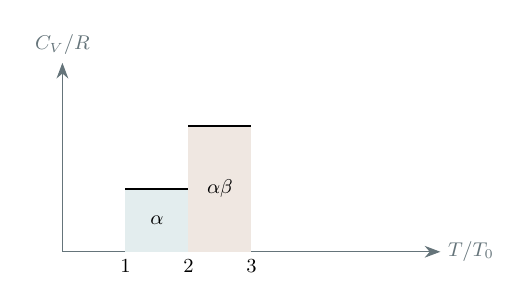
\begin{tikzpicture}[scale=.8,transform shape]
\draw[axis] (0,0)--(6,0) node[right] {$T/T_0$};\draw[axis] (0,0)--(0,3) node[above] {$C_V/R$};\fill[accent!12] (1,0) rectangle (2,1);\fill[warm!15] (2,0) rectangle (3,2);\draw[thick] (1,1)--(2,1);\draw[thick] (2,2)--(3,2);\node at (1.5,.5) {$\alpha$};\node at (2.5,1) {$\alpha\beta$};\node[below] at (1,0) {$1$};\node[below] at (2,0) {$2$};\node[below] at (3,0) {$3$};
\end{tikzpicture}
\figcaption{变图热试2.1V4\quad 等体热量是两块热容量积分面积之和}
\end{minipage}\end{center}

\Needspace{20\baselineskip}
\item 求$B,E$两态的熵差，并说明它们为何在$U$—$T$图上重合。
\textbf{解：}变图热试2.1V5把两态沿$T=2T_0$的等温线连接，体积从$V_0$增至$3V_0/2$。理想气体内能只随温度变化，因此这条等温线上$\Delta U=0$；可逆等温膨胀给$\Delta S_{E B}=\nu R\ln(V_E/V_B)=\nu R\ln(3/2)>0$。两态温度和内能相同，故在投影图中重合，但其体积和熵各不相同。这条辅助等温线用于比较状态，矩形循环仍沿题设的四条边进行。
\begin{center}\begin{minipage}{.98\linewidth}\centering
\begin{tikzpicture}[scale=.8,transform shape]
\draw[axis] (0,0)--(6,0) node[right] {$V$};\draw[axis] (0,0)--(0,3) node[above] {$p$};\draw[traj] plot coordinates {(2.00000000,2.40000000) (2.02500000,2.37037037) (2.05000000,2.34146341) (2.07500000,2.31325301) (2.10000000,2.28571429) (2.12500000,2.25882353) (2.15000000,2.23255814) (2.17500000,2.20689655) (2.20000000,2.18181818) (2.22500000,2.15730337) (2.25000000,2.13333333) (2.27500000,2.10989011) (2.30000000,2.08695652) (2.32500000,2.06451613) (2.35000000,2.04255319) (2.37500000,2.02105263) (2.40000000,2.00000000) (2.42500000,1.97938144) (2.45000000,1.95918367) (2.47500000,1.93939394) (2.50000000,1.92000000) (2.52500000,1.90099010) (2.55000000,1.88235294) (2.57500000,1.86407767) (2.60000000,1.84615385) (2.62500000,1.82857143) (2.65000000,1.81132075) (2.67500000,1.79439252) (2.70000000,1.77777778) (2.72500000,1.76146789) (2.75000000,1.74545455) (2.77500000,1.72972973) (2.80000000,1.71428571) (2.82500000,1.69911504) (2.85000000,1.68421053) (2.87500000,1.66956522) (2.90000000,1.65517241) (2.92500000,1.64102564) (2.95000000,1.62711864) (2.97500000,1.61344538) (3.00000000,1.60000000)};\fill (2,2.4) circle(.04) node[above] {$B$};\fill (3,1.6) circle(.04) node[right] {$E$};\node at (3,-1.5) {$T=2T_0,\quad\Delta S=\nu R\ln(3/2)$};
\end{tikzpicture}
\figcaption{变图热试2.1V5\quad 比较同温不同体积两态的辅助可逆等温路径}
\end{minipage}\end{center}

\Needspace{20\baselineskip}
\item 保持$\alpha$和矩形路径不变，求效率随$\beta$的变化率与高热容量极限。
\textbf{解：}变图热试2.1V6由$A=\alpha(1+\beta)+1$写成$\eta=1/(2A)$。对$\beta$求导，$\mathrm d\eta/\mathrm d\beta=-\alpha/(2A^2)<0$，二阶导数为$\alpha^2/A^3>0$。所以效率随高温热容量增加而下降，曲线向上凸；当$\beta\to\infty$时$\eta\sim1/(2\alpha\beta)$趋零。机械功保持$\nu RT_0/2$，增加的吸热与放热共同反映内部能量的往返交换。
\begin{center}\begin{minipage}{.98\linewidth}\centering
\begin{tikzpicture}[scale=.8,transform shape]
\draw[axis] (0,0)--(10.7,0) node[right] {$\beta$};
\draw[axis] (0,0)--(0,3.2) node[above] {$\eta$};
\node[above] at (5,3.5) {高温热容量增大，效率单调下降并趋向零};
\draw[traj] plot coordinates {(0.000000000,2.800000000) (0.083333333,2.763157895) (0.166666667,2.727272727) (0.250000000,2.692307692) (0.333333333,2.658227848) (0.416666667,2.625000000) (0.500000000,2.592592593) (0.583333333,2.560975610) (0.666666667,2.530120482) (0.750000000,2.500000000) (0.833333333,2.470588235) (0.916666667,2.441860465) (1.000000000,2.413793103) (1.083333333,2.386363636) (1.166666667,2.359550562) (1.250000000,2.333333333) (1.333333333,2.307692308) (1.416666667,2.282608696) (1.500000000,2.258064516) (1.583333333,2.234042553) (1.666666667,2.210526316) (1.750000000,2.187500000) (1.833333333,2.164948454) (1.916666667,2.142857143) (2.000000000,2.121212121) (2.083333333,2.100000000) (2.166666667,2.079207921) (2.250000000,2.058823529) (2.333333333,2.038834951) (2.416666667,2.019230769) (2.500000000,2.000000000) (2.583333333,1.981132075) (2.666666667,1.962616822) (2.750000000,1.944444444) (2.833333333,1.926605505) (2.916666667,1.909090909) (3.000000000,1.891891892) (3.083333333,1.875000000) (3.166666667,1.858407080) (3.250000000,1.842105263) (3.333333333,1.826086957) (3.416666667,1.810344828) (3.500000000,1.794871795) (3.583333333,1.779661017) (3.666666667,1.764705882) (3.750000000,1.750000000) (3.833333333,1.735537190) (3.916666667,1.721311475) (4.000000000,1.707317073) (4.083333333,1.693548387) (4.166666667,1.680000000) (4.250000000,1.666666667) (4.333333333,1.653543307) (4.416666667,1.640625000) (4.500000000,1.627906977) (4.583333333,1.615384615) (4.666666667,1.603053435) (4.750000000,1.590909091) (4.833333333,1.578947368) (4.916666667,1.567164179) (5.000000000,1.555555556) (5.083333333,1.544117647) (5.166666667,1.532846715) (5.250000000,1.521739130) (5.333333333,1.510791367) (5.416666667,1.500000000) (5.500000000,1.489361702) (5.583333333,1.478873239) (5.666666667,1.468531469) (5.750000000,1.458333333) (5.833333333,1.448275862) (5.916666667,1.438356164) (6.000000000,1.428571429) (6.083333333,1.418918919) (6.166666667,1.409395973) (6.250000000,1.400000000) (6.333333333,1.390728477) (6.416666667,1.381578947) (6.500000000,1.372549020) (6.583333333,1.363636364) (6.666666667,1.354838710) (6.750000000,1.346153846) (6.833333333,1.337579618) (6.916666667,1.329113924) (7.000000000,1.320754717) (7.083333333,1.312500000) (7.166666667,1.304347826) (7.250000000,1.296296296) (7.333333333,1.288343558) (7.416666667,1.280487805) (7.500000000,1.272727273) (7.583333333,1.265060241) (7.666666667,1.257485030) (7.750000000,1.250000000) (7.833333333,1.242603550) (7.916666667,1.235294118) (8.000000000,1.228070175) (8.083333333,1.220930233) (8.166666667,1.213872832) (8.250000000,1.206896552) (8.333333333,1.200000000) (8.416666667,1.193181818) (8.500000000,1.186440678) (8.583333333,1.179775281) (8.666666667,1.173184358) (8.750000000,1.166666667) (8.833333333,1.160220994) (8.916666667,1.153846154) (9.000000000,1.147540984) (9.083333333,1.141304348) (9.166666667,1.135135135) (9.250000000,1.129032258) (9.333333333,1.122994652) (9.416666667,1.117021277) (9.500000000,1.111111111) (9.583333333,1.105263158) (9.666666667,1.099476440) (9.750000000,1.093750000) (9.833333333,1.088082902) (9.916666667,1.082474227) (10.000000000,1.076923077)};
\node[below] at (0,-.12) {$1$};
\node[below] at (5,-.12) {$3$};
\node[below] at (10,-.12) {$5$};
\end{tikzpicture}
\figcaption{变图热试2.1V6\quad 高温热容量增大，效率单调下降并趋向零}
\end{minipage}\end{center}

\Needspace{20\baselineskip}
\item 将热容量阶跃温度改为$cT_0$，$1<c<3$，其余矩形路径不变，求效率。
\textbf{解：}变图热试2.1V7从$T_0$加热到$3T_0$的内能增加为$\alpha\nu RT_0[(c-1)+\beta(3-c)]$，上边膨胀功仍为$\nu RT_0$。因此$\eta=1/\{2[\alpha(c-1+\beta(3-c))+1]\}$。分母对$c$的导数为$2\alpha(1-\beta)<0$，所以提高阶跃温度使效率增加；低热容量覆盖的温区扩大，所需正吸热减少。$c=2$得到主解，图中各曲线点按同一分段积分计算。
\begin{center}\begin{minipage}{.98\linewidth}\centering
\begin{tikzpicture}[scale=.8,transform shape]
\draw[axis] (0,0)--(10.7,0) node[right] {$c=T_{\rm step}/T_0$};
\draw[axis] (0,0)--(0,3.2) node[above] {$\eta$};
\node[above] at (5,3.5) {$\alpha=\beta=2$：提高阶跃温度减少吸热};
\draw[traj] plot coordinates {(0.000000000,1.555555556) (0.083333333,1.561338290) (0.166666667,1.567164179) (0.250000000,1.573033708) (0.333333333,1.578947368) (0.416666667,1.584905660) (0.500000000,1.590909091) (0.583333333,1.596958175) (0.666666667,1.603053435) (0.750000000,1.609195402) (0.833333333,1.615384615) (0.916666667,1.621621622) (1.000000000,1.627906977) (1.083333333,1.634241245) (1.166666667,1.640625000) (1.250000000,1.647058824) (1.333333333,1.653543307) (1.416666667,1.660079051) (1.500000000,1.666666667) (1.583333333,1.673306773) (1.666666667,1.680000000) (1.750000000,1.686746988) (1.833333333,1.693548387) (1.916666667,1.700404858) (2.000000000,1.707317073) (2.083333333,1.714285714) (2.166666667,1.721311475) (2.250000000,1.728395062) (2.333333333,1.735537190) (2.416666667,1.742738589) (2.500000000,1.750000000) (2.583333333,1.757322176) (2.666666667,1.764705882) (2.750000000,1.772151899) (2.833333333,1.779661017) (2.916666667,1.787234043) (3.000000000,1.794871795) (3.083333333,1.802575107) (3.166666667,1.810344828) (3.250000000,1.818181818) (3.333333333,1.826086957) (3.416666667,1.834061135) (3.500000000,1.842105263) (3.583333333,1.850220264) (3.666666667,1.858407080) (3.750000000,1.866666667) (3.833333333,1.875000000) (3.916666667,1.883408072) (4.000000000,1.891891892) (4.083333333,1.900452489) (4.166666667,1.909090909) (4.250000000,1.917808219) (4.333333333,1.926605505) (4.416666667,1.935483871) (4.500000000,1.944444444) (4.583333333,1.953488372) (4.666666667,1.962616822) (4.750000000,1.971830986) (4.833333333,1.981132075) (4.916666667,1.990521327) (5.000000000,2.000000000) (5.083333333,2.009569378) (5.166666667,2.019230769) (5.250000000,2.028985507) (5.333333333,2.038834951) (5.416666667,2.048780488) (5.500000000,2.058823529) (5.583333333,2.068965517) (5.666666667,2.079207921) (5.750000000,2.089552239) (5.833333333,2.100000000) (5.916666667,2.110552764) (6.000000000,2.121212121) (6.083333333,2.131979695) (6.166666667,2.142857143) (6.250000000,2.153846154) (6.333333333,2.164948454) (6.416666667,2.176165803) (6.500000000,2.187500000) (6.583333333,2.198952880) (6.666666667,2.210526316) (6.750000000,2.222222222) (6.833333333,2.234042553) (6.916666667,2.245989305) (7.000000000,2.258064516) (7.083333333,2.270270270) (7.166666667,2.282608696) (7.250000000,2.295081967) (7.333333333,2.307692308) (7.416666667,2.320441989) (7.500000000,2.333333333) (7.583333333,2.346368715) (7.666666667,2.359550562) (7.750000000,2.372881356) (7.833333333,2.386363636) (7.916666667,2.400000000) (8.000000000,2.413793103) (8.083333333,2.427745665) (8.166666667,2.441860465) (8.250000000,2.456140351) (8.333333333,2.470588235) (8.416666667,2.485207101) (8.500000000,2.500000000) (8.583333333,2.514970060) (8.666666667,2.530120482) (8.750000000,2.545454545) (8.833333333,2.560975610) (8.916666667,2.576687117) (9.000000000,2.592592593) (9.083333333,2.608695652) (9.166666667,2.625000000) (9.250000000,2.641509434) (9.333333333,2.658227848) (9.416666667,2.675159236) (9.500000000,2.692307692) (9.583333333,2.709677419) (9.666666667,2.727272727) (9.750000000,2.745098039) (9.833333333,2.763157895) (9.916666667,2.781456954) (10.000000000,2.800000000)};
\node[below] at (0,-.12) {$1$};
\node[below] at (5,-.12) {$2$};
\node[below] at (10,-.12) {$3$};
\end{tikzpicture}
\figcaption{变图热试2.1V7\quad $\alpha=\beta=2$：提高阶跃温度减少吸热}
\end{minipage}\end{center}

\Needspace{20\baselineskip}
\item 沿等压过程从$T_0$加热到$3T_0$，求总热量，并与等体加热比较。
\textbf{解：}变图热试2.1V8中压强保持$p_0$，状态方程给体积从$V_0$增至$3V_0$，膨胀功为$p_0(3V_0-V_0)=2\nu RT_0$。内能变化与等体加热相同，为$\alpha(1+\beta)\nu RT_0$，所以$Q_p=[\alpha(1+\beta)+2]\nu RT_0$。等体过程的全部热量进入内能，等压过程还提供这项膨胀功，二者热量之差为$2\nu RT_0$，图中的不同路径将温度端点和机械功分别表示。
\begin{center}\begin{minipage}{.98\linewidth}\centering
\begin{tikzpicture}[scale=.8,transform shape]
\draw[axis] (0,0)--(6,0) node[right] {$V$};\draw[axis] (0,0)--(0,3) node[above] {$p$};\draw[traj] (1,1)--(3,1);\draw[traj,dashed] (1,1)--(1,3);\node[below] at (1,1) {$T_0$};\node[right] at (3,1) {$3T_0$等压};\node[above] at (1,3) {$3T_0$等体};\node at (3,-1.5) {$Q_p-Q_V=2\nu RT_0$};
\end{tikzpicture}
\figcaption{变图热试2.1V8\quad 同温度端点的两条加热路径具有相同内能变化与不同机械功}
\end{minipage}\end{center}
\end{enumerate}

\Needspace{13\baselineskip}

\pdfbookmark[2]{第 2 题 有限热源的最大作功与相变卡诺循环}{q2}

\section*{第 2 题\quad 有限热源的最大作功与相变卡诺循环}\label{q:2}


两个物体的初温为$T_1>T_2>0$，各自热容量均为常量$C$。以小型可逆热机在两者之间连续工作，每轮换热足够少，可忽略一轮内部热源温度的变化；整体与外界绝热。
\begin{enumerate}
\item 求热机对外总作功的最大值和最终共同温度。
\item 第一轮工质为$\nu$ mol。高温等温过程从$T_1$下的全液态开始，等温等压吸热$L$后全部汽化为体积$V_1$的气体，再在$T_1$等温膨胀至$V_2$。随后经可逆绝热及$T_2$等温过程返回初态。气相除两相共存区外可视为理想气体。定性画出一种能闭合的$p$--$V$和$T$--$S$循环，求第一轮功。这里$L$为全部工质汽化吸收的总潜热。
\end{enumerate}


\begin{center}\begin{minipage}{.98\linewidth}\centering
\begin{tikzpicture}[scale=.9,transform shape]

\draw[object,fill=warm!8] (0,2.8) rectangle (2,4);
\draw[object,fill=accent!8] (0,-.4) rectangle (2,.8);
\draw[object,fill=muted!8] (3.5,1.2) rectangle (5.3,2.4);
\node[align=center] at (1,3.4) {热物体\\$T_1,C$};
\node[align=center] at (1,.2) {冷物体\\$T_2,C$};
\node at (4.4,1.8) {可逆热机};
\draw[force] (2,3.4)--(4.4,3.4)--(4.4,2.45);
\node[above] at (3.2,3.4) {$Q_h$};
\draw[force] (4.4,1.15)--(4.4,.2)--(2,.2);
\node[below] at (3.2,.2) {$Q_c$};
\draw[motion] (5.35,1.8)--(6.8,1.8) node[right] {$W$};
\draw[guide,rounded corners] (-.3,-.7) rectangle (6,4.3);
\node[below] at (2.8,-.8) {整体绝热，仅向外输出功};

\end{tikzpicture}
\figcaption{图热试2.2\quad 两物体温度随连续微小循环改变，整体能量减少量为输出功。}
\end{minipage}\end{center}

\Needspace{8\baselineskip}

\pdfbookmark[3]{题型定位}{q2-h0}

\subsection*{题型定位}

第一问把无数微小可逆循环累计，用两个有限物体的总能量和总熵确定最大功；第二问只取第一次循环，把本轮热源温度近似看作常量，用相变热与气相等温膨胀热确定熵宽。两个问题共享可逆性，但分别描述热源温度的连续演变与一轮工质的状态变化。

\Needspace{8\baselineskip}

\pdfbookmark[3]{知识点}{q2-h1}

\subsection*{知识点}

有限物体的熵变为$C\ln(T_f/T_i)$，整体绝热时输出的机械功等于总内能减少。可逆极限总熵保持不变，熵产生使相同初态对应更高终温和更少机械功。相变潜热与可逆等温热量都满足$Q=T\Delta S$，绝热段保持熵不变。卡诺循环在$T$—$S$图上的面积为温差乘熵宽，气相等温部分另由$\int p\mathrm dV$计算。

\Needspace{8\baselineskip}

\pdfbookmark[3]{物理图像}{q2-h2}

\subsection*{物理图像}

题图把两个有限物体与热机置于绝热围壁内，只向外输出功。解图热试2.2A中热物体降温、冷物体升温，二者沿乘积不变的关系接近几何平均温度。图B的$AF$是高温汽化平台，$FB$是高温气相等温膨胀；图C把二者接在同一条水平等温边上。图D则把热源逐渐等温化的过程与累计输出功一一对应。

\Needspace{8\baselineskip}

\pdfbookmark[3]{解题入口}{q2-h3}

\subsection*{解题入口}

第一问从能量式$W=C(T_1+T_2-2T_e)$入手，输出的机械功越大，共同终温越低，再由总熵不减求最低终温。第二问沿图B的高温边分出$AF$与$FB$，分别算吸热$L$和$\nu RT_1\ln(V_2/V_1)$；把吸热除以$T_1$得到图C的熵宽，再以温差乘熵宽求功。

\Needspace{8\baselineskip}

\pdfbookmark[3]{标准解法}{q2-h4}

\subsection*{标准解法}


图热试2.2把两个有限物体与热机一起放入绝热边界。总作功最大时，过程可逆且最终不再有可供热机利用的温差，故共同终温记为$T_e$。
两物体的热容量有限，随着每轮取热、放热，热物体温度连续下降，冷物体温度连续上升。若停机时仍有温差，可再作一个可逆微小循环并输出正功，故极限停机条件是共同温度。热机完整循环后回到本轮初态，累计内能变化为零，输出功由两个物体的能量减少提供。两物体分别放、吸热
\[
Q_h=C(T_1-T_e),\qquad Q_c=C(T_e-T_2),
\]
整体能量守恒给
\[
W=C(T_1+T_2-2T_e).
\]
可逆热机每轮工质熵变为零，两个物体的总熵保持不变：
\[
C\ln\frac{T_e}{T_1}+C\ln\frac{T_e}{T_2}=0,
\qquad
\boxed{T_e=\sqrt{T_1T_2}}.
\]
于是
\[
\boxed{W_{\max}=C(T_1+T_2-2\sqrt{T_1T_2})
=C(\sqrt{T_1}-\sqrt{T_2})^2}.
\]
\begin{center}\begin{minipage}{.98\linewidth}\centering
\begin{tikzpicture}[scale=.8,transform shape]
\draw[axis] (0,0)--(10.7,0) node[right] {$z=(4T_2-T_h)/(2T_2)$};
\draw[axis] (0,0)--(0,3.2) node[above] {$T_h/T_2,\ T_c/T_2$};\foreach \y/\lab in {0/1,.9/2,1.8/3,2.7/4}{\draw[thin] (0,\y)--(-.08,\y) node[left] {$\lab$};}
\node[above] at (5,3.5) {$T_1=4T_2$：实线热物体，虚线冷物体};
\draw[traj] plot coordinates {(0.000000000,2.700000000) (0.083333333,2.685000000) (0.166666667,2.670000000) (0.250000000,2.655000000) (0.333333333,2.640000000) (0.416666667,2.625000000) (0.500000000,2.610000000) (0.583333333,2.595000000) (0.666666667,2.580000000) (0.750000000,2.565000000) (0.833333333,2.550000000) (0.916666667,2.535000000) (1.000000000,2.520000000) (1.083333333,2.505000000) (1.166666667,2.490000000) (1.250000000,2.475000000) (1.333333333,2.460000000) (1.416666667,2.445000000) (1.500000000,2.430000000) (1.583333333,2.415000000) (1.666666667,2.400000000) (1.750000000,2.385000000) (1.833333333,2.370000000) (1.916666667,2.355000000) (2.000000000,2.340000000) (2.083333333,2.325000000) (2.166666667,2.310000000) (2.250000000,2.295000000) (2.333333333,2.280000000) (2.416666667,2.265000000) (2.500000000,2.250000000) (2.583333333,2.235000000) (2.666666667,2.220000000) (2.750000000,2.205000000) (2.833333333,2.190000000) (2.916666667,2.175000000) (3.000000000,2.160000000) (3.083333333,2.145000000) (3.166666667,2.130000000) (3.250000000,2.115000000) (3.333333333,2.100000000) (3.416666667,2.085000000) (3.500000000,2.070000000) (3.583333333,2.055000000) (3.666666667,2.040000000) (3.750000000,2.025000000) (3.833333333,2.010000000) (3.916666667,1.995000000) (4.000000000,1.980000000) (4.083333333,1.965000000) (4.166666667,1.950000000) (4.250000000,1.935000000) (4.333333333,1.920000000) (4.416666667,1.905000000) (4.500000000,1.890000000) (4.583333333,1.875000000) (4.666666667,1.860000000) (4.750000000,1.845000000) (4.833333333,1.830000000) (4.916666667,1.815000000) (5.000000000,1.800000000) (5.083333333,1.785000000) (5.166666667,1.770000000) (5.250000000,1.755000000) (5.333333333,1.740000000) (5.416666667,1.725000000) (5.500000000,1.710000000) (5.583333333,1.695000000) (5.666666667,1.680000000) (5.750000000,1.665000000) (5.833333333,1.650000000) (5.916666667,1.635000000) (6.000000000,1.620000000) (6.083333333,1.605000000) (6.166666667,1.590000000) (6.250000000,1.575000000) (6.333333333,1.560000000) (6.416666667,1.545000000) (6.500000000,1.530000000) (6.583333333,1.515000000) (6.666666667,1.500000000) (6.750000000,1.485000000) (6.833333333,1.470000000) (6.916666667,1.455000000) (7.000000000,1.440000000) (7.083333333,1.425000000) (7.166666667,1.410000000) (7.250000000,1.395000000) (7.333333333,1.380000000) (7.416666667,1.365000000) (7.500000000,1.350000000) (7.583333333,1.335000000) (7.666666667,1.320000000) (7.750000000,1.305000000) (7.833333333,1.290000000) (7.916666667,1.275000000) (8.000000000,1.260000000) (8.083333333,1.245000000) (8.166666667,1.230000000) (8.250000000,1.215000000) (8.333333333,1.200000000) (8.416666667,1.185000000) (8.500000000,1.170000000) (8.583333333,1.155000000) (8.666666667,1.140000000) (8.750000000,1.125000000) (8.833333333,1.110000000) (8.916666667,1.095000000) (9.000000000,1.080000000) (9.083333333,1.065000000) (9.166666667,1.050000000) (9.250000000,1.035000000) (9.333333333,1.020000000) (9.416666667,1.005000000) (9.500000000,0.990000000) (9.583333333,0.975000000) (9.666666667,0.960000000) (9.750000000,0.945000000) (9.833333333,0.930000000) (9.916666667,0.915000000) (10.000000000,0.900000000)};
\draw[dashed,thick,color=warm] plot coordinates {(0.000000000,0.000000000) (0.083333333,0.003765690) (0.166666667,0.007563025) (0.250000000,0.011392405) (0.333333333,0.015254237) (0.416666667,0.019148936) (0.500000000,0.023076923) (0.583333333,0.027038627) (0.666666667,0.031034483) (0.750000000,0.035064935) (0.833333333,0.039130435) (0.916666667,0.043231441) (1.000000000,0.047368421) (1.083333333,0.051541850) (1.166666667,0.055752212) (1.250000000,0.060000000) (1.333333333,0.064285714) (1.416666667,0.068609865) (1.500000000,0.072972973) (1.583333333,0.077375566) (1.666666667,0.081818182) (1.750000000,0.086301370) (1.833333333,0.090825688) (1.916666667,0.095391705) (2.000000000,0.100000000) (2.083333333,0.104651163) (2.166666667,0.109345794) (2.250000000,0.114084507) (2.333333333,0.118867925) (2.416666667,0.123696682) (2.500000000,0.128571429) (2.583333333,0.133492823) (2.666666667,0.138461538) (2.750000000,0.143478261) (2.833333333,0.148543689) (2.916666667,0.153658537) (3.000000000,0.158823529) (3.083333333,0.164039409) (3.166666667,0.169306931) (3.250000000,0.174626866) (3.333333333,0.180000000) (3.416666667,0.185427136) (3.500000000,0.190909091) (3.583333333,0.196446701) (3.666666667,0.202040816) (3.750000000,0.207692308) (3.833333333,0.213402062) (3.916666667,0.219170984) (4.000000000,0.225000000) (4.083333333,0.230890052) (4.166666667,0.236842105) (4.250000000,0.242857143) (4.333333333,0.248936170) (4.416666667,0.255080214) (4.500000000,0.261290323) (4.583333333,0.267567568) (4.666666667,0.273913043) (4.750000000,0.280327869) (4.833333333,0.286813187) (4.916666667,0.293370166) (5.000000000,0.300000000) (5.083333333,0.306703911) (5.166666667,0.313483146) (5.250000000,0.320338983) (5.333333333,0.327272727) (5.416666667,0.334285714) (5.500000000,0.341379310) (5.583333333,0.348554913) (5.666666667,0.355813953) (5.750000000,0.363157895) (5.833333333,0.370588235) (5.916666667,0.378106509) (6.000000000,0.385714286) (6.083333333,0.393413174) (6.166666667,0.401204819) (6.250000000,0.409090909) (6.333333333,0.417073171) (6.416666667,0.425153374) (6.500000000,0.433333333) (6.583333333,0.441614907) (6.666666667,0.450000000) (6.750000000,0.458490566) (6.833333333,0.467088608) (6.916666667,0.475796178) (7.000000000,0.484615385) (7.083333333,0.493548387) (7.166666667,0.502597403) (7.250000000,0.511764706) (7.333333333,0.521052632) (7.416666667,0.530463576) (7.500000000,0.540000000) (7.583333333,0.549664430) (7.666666667,0.559459459) (7.750000000,0.569387755) (7.833333333,0.579452055) (7.916666667,0.589655172) (8.000000000,0.600000000) (8.083333333,0.610489510) (8.166666667,0.621126761) (8.250000000,0.631914894) (8.333333333,0.642857143) (8.416666667,0.653956835) (8.500000000,0.665217391) (8.583333333,0.676642336) (8.666666667,0.688235294) (8.750000000,0.700000000) (8.833333333,0.711940299) (8.916666667,0.724060150) (9.000000000,0.736363636) (9.083333333,0.748854962) (9.166666667,0.761538462) (9.250000000,0.774418605) (9.333333333,0.787500000) (9.416666667,0.800787402) (9.500000000,0.814285714) (9.583333333,0.828000000) (9.666666667,0.841935484) (9.750000000,0.856097561) (9.833333333,0.870491803) (9.916666667,0.885123967) (10.000000000,0.900000000)};
\node[below] at (0,-.12) {$0$};
\node[below] at (5,-.12) {$1/2$};
\node[below] at (10,-.12) {$1$};
\end{tikzpicture}
\figcaption{解图热试2.2A\quad $T_1=4T_2$：实线热物体，虚线冷物体}
\end{minipage}\end{center}
解图热试2.2A中两个温度逐渐靠拢；可逆运行的冷物体温度始终满足$T_c=T_1T_2/T_h$。如果有不可逆性，最终总熵满足
\[
C\ln\frac{T_e^2}{T_1T_2}\ge0,
\]
因$C>0$且对数单调，熵不减给共同终温的下限；可逆循环使总熵产生为零，恰好达到此下限。所以$T_e\ge\sqrt{T_1T_2}$，代回能量式便知作功不超过上式。\begin{center}\begin{minipage}{.98\linewidth}\centering
\begin{tikzpicture}[scale=.8,transform shape]
\draw[axis] (0,0)--(10.7,0) node[right] {$z$};
\draw[axis] (0,0)--(0,3.2) node[above] {$W/(CT_2)$};
\node[above] at (5,3.5) {两物体沿可逆温度关系接近时的累计功};
\draw[traj] plot coordinates {(0.000000000,0.000000000) (0.083333333,0.034951185) (0.166666667,0.069803922) (0.250000000,0.104556962) (0.333333333,0.139209040) (0.416666667,0.173758865) (0.500000000,0.208205128) (0.583333333,0.242546495) (0.666666667,0.276781609) (0.750000000,0.310909091) (0.833333333,0.344927536) (0.916666667,0.378835517) (1.000000000,0.412631579) (1.083333333,0.446314244) (1.166666667,0.479882006) (1.250000000,0.513333333) (1.333333333,0.546666667) (1.416666667,0.579880419) (1.500000000,0.612972973) (1.583333333,0.645942685) (1.666666667,0.678787879) (1.750000000,0.711506849) (1.833333333,0.744097859) (1.916666667,0.776559140) (2.000000000,0.808888889) (2.083333333,0.841085271) (2.166666667,0.873146417) (2.250000000,0.905070423) (2.333333333,0.936855346) (2.416666667,0.968499210) (2.500000000,1.000000000) (2.583333333,1.031355662) (2.666666667,1.062564103) (2.750000000,1.093623188) (2.833333333,1.124530744) (2.916666667,1.155284553) (3.000000000,1.185882353) (3.083333333,1.216321839) (3.166666667,1.246600660) (3.250000000,1.276716418) (3.333333333,1.306666667) (3.416666667,1.336448911) (3.500000000,1.366060606) (3.583333333,1.395499154) (3.666666667,1.424761905) (3.750000000,1.453846154) (3.833333333,1.482749141) (3.916666667,1.511468048) (4.000000000,1.540000000) (4.083333333,1.568342059) (4.166666667,1.596491228) (4.250000000,1.624444444) (4.333333333,1.652198582) (4.416666667,1.679750446) (4.500000000,1.707096774) (4.583333333,1.734234234) (4.666666667,1.761159420) (4.750000000,1.787868852) (4.833333333,1.814358974) (4.916666667,1.840626151) (5.000000000,1.866666667) (5.083333333,1.892476723) (5.166666667,1.918052434) (5.250000000,1.943389831) (5.333333333,1.968484848) (5.416666667,1.993333333) (5.500000000,2.017931034) (5.583333333,2.042273603) (5.666666667,2.066356589) (5.750000000,2.090175439) (5.833333333,2.113725490) (5.916666667,2.137001972) (6.000000000,2.160000000) (6.083333333,2.182714571) (6.166666667,2.205140562) (6.250000000,2.227272727) (6.333333333,2.249105691) (6.416666667,2.270633947) (6.500000000,2.291851852) (6.583333333,2.312753623) (6.666666667,2.333333333) (6.750000000,2.353584906) (6.833333333,2.373502110) (6.916666667,2.393078556) (7.000000000,2.412307692) (7.083333333,2.431182796) (7.166666667,2.449696970) (7.250000000,2.467843137) (7.333333333,2.485614035) (7.416666667,2.503002208) (7.500000000,2.520000000) (7.583333333,2.536599553) (7.666666667,2.552792793) (7.750000000,2.568571429) (7.833333333,2.583926941) (7.916666667,2.598850575) (8.000000000,2.613333333) (8.083333333,2.627365967) (8.166666667,2.640938967) (8.250000000,2.654042553) (8.333333333,2.666666667) (8.416666667,2.678800959) (8.500000000,2.690434783) (8.583333333,2.701557178) (8.666666667,2.712156863) (8.750000000,2.722222222) (8.833333333,2.731741294) (8.916666667,2.740701754) (9.000000000,2.749090909) (9.083333333,2.756895674) (9.166666667,2.764102564) (9.250000000,2.770697674) (9.333333333,2.776666667) (9.416666667,2.781994751) (9.500000000,2.786666667) (9.583333333,2.790666667) (9.666666667,2.793978495) (9.750000000,2.796585366) (9.833333333,2.798469945) (9.916666667,2.799614325) (10.000000000,2.800000000)};
\node[below] at (0,-.12) {$0$};
\node[below] at (5,-.12) {$1/2$};
\node[below] at (10,-.12) {$1$};
\end{tikzpicture}
\figcaption{解图热试2.2D\quad 两物体沿可逆温度关系接近时的累计功}
\end{minipage}\end{center}
图A、图D用$T_1=4T_2$示例，横坐标$z=(4T_2-T_h)/(2T_2)$从0增加到1。热物体温度从$4T_2$降到$2T_2$，冷物体温度从$T_2$升到$2T_2$，输出功从0增到$CT_2$。微小热量也能给出这条关系：若高温物体减少$-C\mathrm dT_h>0$的热量，可逆热机向冷物体放出$C\mathrm dT_c=-(T_c/T_h)C\mathrm dT_h$，于是$\mathrm d\ln T_h+\mathrm d\ln T_c=0$，沿途保持$T_hT_c=T_1T_2$。

直接接触、不取功时，终温为$(T_1+T_2)/2$；这比可逆取功的终温高。

直接接触的总输出功为零，初始总内能只能在两物体之间重新分配，因而给算术平均。可逆取功则把一部分能量送到系统之外，终温较低；两种终态之间的内能差是$2C[(T_1+T_2)/2-\sqrt{T_1T_2}]$，正好等于最大功。

第（2）问仅讨论第一轮，两个物体在这一轮近似为恒温热源。解图热试2.2B用$A$表示高温全液初态，$F$表示刚全部汽化，$B$表示高温等温膨胀终点。$AF$为汽化平台，$FB$为理想气体等温膨胀。
\begin{center}\begin{minipage}{.98\linewidth}\centering
\begin{tikzpicture}[scale=.85,transform shape]

\draw[axis] (0,0)--(6.7,0) node[right] {$V$};
\draw[axis] (0,0)--(0,4.8) node[above] {$p$};
\draw[traj] (.7,4)--(2.5,4);
\draw[traj,domain=2.5:4,samples=45] plot (\x,{10/\x});
\draw[motion,domain=4:5.59017,samples=60] plot (\x,{2.5*(4/\x)^(5/3)});
\draw[traj,domain=4.44444:5.59017,samples=40] plot (\x,{8/\x});
\draw[traj] (4.44444,1.8)--(1.2,1.8);
\draw[motion] (1.2,1.8) to[out=110,in=-100] (.7,4);
\draw[motion] (1.1,4)--(1.8,4);
\draw[motion] (3,3.333)--(3.5,2.857);
\draw[motion] (5.3,1.509)--(4.85,1.649);
\draw[motion] (3.8,1.8)--(3.1,1.8);
\foreach \x/\y/\lab/\pos in {.7/4/A/above left,2.5/4/F/above,4/2.5/B/above right,5.59017/1.43108/C/right,4.44444/1.8/G/above,1.2/1.8/D/below left}{\fill (\x,\y) circle (1.4pt) node[\pos] {$\lab$};}
\node[above] at (1.6,4.5) {汽化平台，$T_1$};
\node[below] at (2.7,1.8) {部分凝结，$T_2$};
\draw[guide] (2.5,0)--(2.5,4);\node[below] at (2.5,0) {$V_1$};
\draw[guide] (4,0)--(4,2.5);\node[below] at (4,0) {$V_2$};

\end{tikzpicture}
\figcaption{解图热试2.2B\quad 一种定性闭合循环：低温端D按$S_D=S_A$选取为两相态。}
\end{minipage}\end{center}
沿$AF$，液气两相在温度$T_1$和饱和压强下平衡，吸热同时增加内能并推动相界面与活塞；完成汽化后，$F$的体积为$V_1$。沿$FB$，气相内能因温度不变而保持不变，吸热全部用于体积功。高温过程吸热的两部分为
\[
Q_{AF}=L,\qquad
Q_{FB}=\int_{V_1}^{V_2}\frac{\nu RT_1}{V}\,\mathrm dV
=\nu RT_1\ln\frac{V_2}{V_1}.
\]
因此
\[
\boxed{Q_h^{(1)}=L+\nu RT_1\ln\frac{V_2}{V_1}}.
\]
潜热$L$是相变过程中吸收的总热量，第一定律把它分成内能增加与汽化平台下的体积功$p_{\rm sat}\Delta V$。

由$B$沿可逆绝热线降至温度$T_2$的$C$态，再等温压缩至$D$，最后绝热返回$A$。图中选取一种低温等温线上先作气相压缩$CG$、再在$GD$部分凝结的情形，$D$可以是两相共存态；用绝热段$DA$保持$S_D=S_A$，其物态由低温饱和熵与$S_A$的位置关系决定。具体物性还允许其他闭合情形：低温压缩可先经过纯气相再全部凝结，也可从低温等温段开始就处于两相共存区并继续凝结；若$S_D=S_A$落在两相区，便止于部分凝结；若落在纯气相区，压缩终点仍为气体。各情形都由同一条等熵线选定返回初态的终点。若 $D$ 在解图热试2.2B的两相水平段内，记 $S_f(T_2)$、$S_g(T_2)$ 为同一份工质全为饱和液体、全为饱和蒸气时的熵。总熵按质量分配相加，蒸气质量分数 $x_D$ 满足
\[
S_A=S_D=(1-x_D)S_f(T_2)+x_D S_g(T_2),
\qquad
x_D=\frac{S_A-S_f(T_2)}{S_g(T_2)-S_f(T_2)} .
\]
沿低温等温段的熵轴，$x_D$ 就是饱和液端到 $D$ 的距离占整段的比例。两相区内 $0\le x_D\le1$。
\begin{center}\begin{minipage}{.98\linewidth}\centering
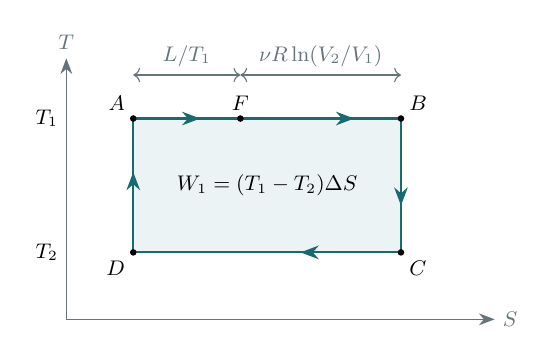
\begin{tikzpicture}[scale=.85,transform shape]

\fill[accent!8] (1,1)--(1,3)--(5,3)--(5,1)--cycle;
\draw[axis] (0,0)--(6.4,0) node[right] {$S$};
\draw[axis] (0,0)--(0,3.9) node[above] {$T$};
\draw[traj] (1,3)--(5,3)--(5,1)--(1,1)--cycle;
\draw[motion] (1.5,3)--(2,3);\draw[motion] (3.4,3)--(4.3,3);
\draw[motion] (5,2.6)--(5,1.7);\draw[motion] (4.4,1)--(3.5,1);
\draw[motion] (1,1.4)--(1,2.2);
\foreach \x/\y/\lab/\pos in {1/3/A/above left,2.6/3/F/above,5/3/B/above right,5/1/C/below right,1/1/D/below left}{\fill (\x,\y) circle (1.4pt) node[\pos] {$\lab$};}
\node[left] at (0,3) {$T_1$};\node[left] at (0,1) {$T_2$};
\draw[axis,<->] (1,3.65)--(2.6,3.65) node[midway,above] {$L/T_1$};
\draw[axis,<->] (2.6,3.65)--(5,3.65) node[midway,above] {$\nu R\ln(V_2/V_1)$};
\node at (3,2) {$W_1=(T_1-T_2)\Delta S$};

\end{tikzpicture}
\figcaption{解图热试2.2C\quad 熵宽含汽化与气相膨胀两部分，围成面积即第一轮功。}
\end{minipage}\end{center}
在所画的例子中，低温压缩先沿气相等温线$CG$减小体积，再在饱和压强下沿$GD$凝结一部分气体。由$S_D=S_A$选择停止凝结的位置，再绝热压缩升温返回$A$。饱和熵、液相比热和状态方程共同决定等熵线落在气相区、两相区或液相区；图B选择与这一闭合关系相容的一种定性情形。气相绝热段$BC$若有常量$\gamma$，还满足$T_1V_2^{\gamma-1}=T_2V_C^{\gamma-1}$，因此$V_C>V_2$，与图中向右下的膨胀方向相同。

解图热试2.2C中$AFB$在$T_1$水平线上，$CD$在$T_2$水平线上，两条绝热线竖直。高温等温边的总熵宽为
\[
\Delta S=\frac{L}{T_1}+\nu R\ln\frac{V_2}{V_1}.
\]
因此低温放热量$Q_c^{(1)}=T_2\Delta S$，第一轮净功等于矩形面积：
\[
\boxed{W_1=(T_1-T_2)\Delta S
=\left(1-\frac{T_2}{T_1}\right)
\left(L+\nu RT_1\ln\frac{V_2}{V_1}\right)}.
\]
求功所需的低温放热量由$T_2\Delta S$直接给出，凝结份额则在给出具体物性后按等熵终点求取。工质的饱和曲线、液相比热等数据未给出，$p$--$V$图只能定性画一种满足熵闭合条件的情形；$T$--$S$图及第一轮功则由可逆性和总吸热确定。
沿$AF$的熵增为$L/T_1$，沿$FB$的熵增为$\nu R\ln(V_2/V_1)$，两部分在图C的高温边上相接。沿$BC$的温度降低而熵保持不变；沿$CD$的温度固定而熵减少同样的$\Delta S$；沿$DA$熵保持不变而温度升高。这四段变化使工质恢复最初的温度、熵和物态，输出功就是吸热与放热之差。随着后续循环推进，热、冷物体温度逐步改变，每轮都在该轮的两端温度间工作，累计后才得到第一问的最大功。



\Needspace{8\baselineskip}

\pdfbookmark[3]{关键洞察}{q2-h5}

\subsection*{关键洞察}

热源的温差能够逐渐转成机械功，直接热接触则把相同温差用于不可逆的热传递。前者的可逆终温为几何平均，后者的无功终温为算术平均。相变与气相膨胀在$p$—$V$图上形状不同，但它们在高温等温边上的熵增都由热量除以$T_1$给出。低温终点按$S_D=S_A$选取，相变份额由具体物性的饱和熵决定。

\Needspace{8\baselineskip}

\pdfbookmark[3]{易错点}{q2-h6}

\subsection*{易错点}

有限热源的温度随运行改变，累计热量与功使用每一时刻的温度关系，初始卡诺效率只属于第一轮近似。汽化潜热$L$已经是总吸热，其中包括平台阶段的体积功；第一定律把它分为内能变化和作功。返回初态的可逆绝热线保持$S_D=S_A$，低温等温压缩停在哪里由这条等熵线决定。$T$—$S$图上的两条竖边是绝热过程，高、低温水平边各有相同熵宽。

\Needspace{8\baselineskip}

\pdfbookmark[3]{课堂讲解建议}{q2-h7}

\subsection*{课堂讲解建议}

先问热机在热、冷物体仍有温差时能否再做一个微小循环，让学生指出温差消失时，后续热机循环的可取功也随之消失。写出能量式后，先用熵不等式说明终温的下限，再说明可逆循环达到等号。取$T_1/T_2=4$比较可逆终温$2T_2$和直接接触终温$2.5T_2$，把内能差对应到输出功。

画第一轮时先标出$A,F,B$，让学生逐段说明物态、温度和吸热。再把这些点映射到图C，高温边的水平长度分别为$L/T_1$和$\nu R\ln(V_2/V_1)$。从$B$画竖直线到$C$，从$A$画竖直线到$D$，用熵坐标选低温压缩终点，最后以面积求功。可继续追问加入少量熵产生后终温和输出功怎样变化。

\Needspace{8\baselineskip}

\pdfbookmark[3]{变式训练}{q2-h8}

\subsection*{变式训练}

\begin{enumerate}
\Needspace{20\baselineskip}
\item 两物体热容量改为不同常量$C_h,C_c$，求可逆终温和最大功。
\textbf{解：}变图热试2.2V1对两个物体分别写熵变，$C_h\ln(T_e/T_1)+C_c\ln(T_e/T_2)=0$。因此$\ln T_e=(C_h\ln T_1+C_c\ln T_2)/(C_h+C_c)$，即$T_e=(T_1^{C_h}T_2^{C_c})^{1/(C_h+C_c)}$。总能量减少给$W_{\max}=C_hT_1+C_cT_2-(C_h+C_c)T_e$。较大热容量对应更大的对数权重，终温向该物体的初温靠近；当两热容量相等时回到几何平均。
\begin{center}\begin{minipage}{.98\linewidth}\centering
\begin{tikzpicture}[scale=.8,transform shape]
\node[draw,minimum width=2.4cm,minimum height=1cm] (h) at (0,1) {$C_h,T_1$};\node[draw] (e) at (4,1) {可逆热机};\node[draw,minimum width=2.4cm,minimum height=1cm] (c) at (8,1) {$C_c,T_2$};\draw[motion] (h)--(e);\draw[motion] (e)--(c);\node at (4,-1) {$T_e=T_1^{C_h/(C_h+C_c)}T_2^{C_c/(C_h+C_c)}$};
\end{tikzpicture}
\figcaption{变图热试2.2V1\quad 不同热容量使终温成为带热容量权重的几何平均}
\end{minipage}\end{center}

\Needspace{20\baselineskip}
\item 第一轮汽化完成后立即沿绝热线降温，即$V_2=V_1$，求功和熵宽。
\textbf{解：}变图热试2.2V2中高温等温边只保留$AF$汽化阶段。因为$\ln(V_2/V_1)=0$，本轮高温吸热为$L$，熵增为$L/T_1$。低温等温边放热$T_2L/T_1$，故$W_1=L-T_2L/T_1=(1-T_2/T_1)L$。$T$—$S$矩形仍有有限宽度$L/T_1$，高温边虽没有继续作气相等温膨胀，汽化吸热仍能驱动循环输出功。
\begin{center}\begin{minipage}{.98\linewidth}\centering
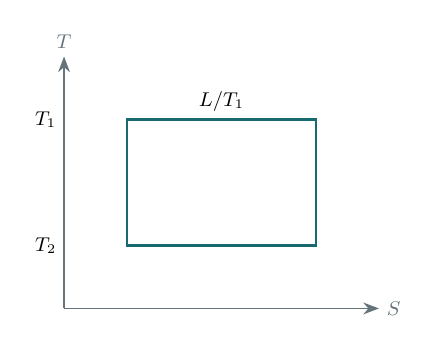
\begin{tikzpicture}[scale=.8,transform shape]
\draw[axis] (0,0)--(5,0) node[right] {$S$};\draw[axis] (0,0)--(0,4) node[above] {$T$};\draw[traj] (1,3)--(4,3)--(4,1)--(1,1)--cycle;\node[above] at (2.5,3) {$L/T_1$};\node[left] at (0,3) {$T_1$};\node[left] at (0,1) {$T_2$};
\end{tikzpicture}
\figcaption{变图热试2.2V2\quad 仅有汽化吸热时，卡诺矩形仍具有潜热产生的熵宽}
\end{minipage}\end{center}

\Needspace{20\baselineskip}
\item 去掉相变，令工质在高温边全部为理想气体，求本轮功。
\textbf{解：}变图热试2.2V3只保留气相等温膨胀，取$L=0$。高温吸热为$\nu RT_1\ln(V_2/V_1)$，熵宽为$\nu R\ln(V_2/V_1)$，所以$W_1=\nu R(T_1-T_2)\ln(V_2/V_1)$。气相两条绝热线若有恒定$\gamma$，给$T_1V_2^{\gamma-1}=T_2V_C^{\gamma-1}$与$T_1V_1^{\gamma-1}=T_2V_D^{\gamma-1}$，相除可得$V_C/V_D=V_2/V_1$，两等温边熵宽相同。
\begin{center}\begin{minipage}{.98\linewidth}\centering
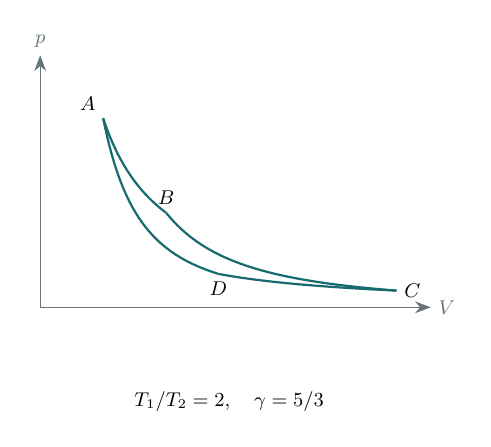
\begin{tikzpicture}[scale=.8,transform shape]
\draw[axis] (0,0)--(6.2,0) node[right] {$V$};\draw[axis] (0,0)--(0,4) node[above] {$p$};\draw[traj,domain=1:2,samples=61] plot (\x,{3/\x});\draw[traj,domain=2:5.656854249,samples=61] plot (\x,{1.5*pow(2,5/3)/pow(\x,5/3)});\draw[traj,domain=2.828427125:5.656854249,samples=61] plot (\x,{1.5/\x});\draw[traj,domain=1:2.828427125,samples=61] plot (\x,{3/pow(\x,5/3)});\node[above left] at (1,3) {$A$};\node[above] at (2,1.5) {$B$};\node[right] at (5.656854249,.265165043) {$C$};\node[below] at (2.828427125,.530330086) {$D$};\node at (3,-1.5) {$T_1/T_2=2,\quad\gamma=5/3$};
\end{tikzpicture}
\figcaption{变图热试2.2V3\quad 两条理想气体等温线与两条等熵线组成闭合卡诺循环}
\end{minipage}\end{center}

\Needspace{20\baselineskip}
\item 可逆取功在$T_h>T_c$时提前停机，求已取功和剩余可取功。
\textbf{解：}变图热试2.2V4中沿途总熵不变，故$T_hT_c=T_1T_2$。已取功为$W=C(T_1+T_2-T_h-T_c)$。继续运行到共同温度$\sqrt{T_1T_2}$还能取出$W_{\rm rem}=C(T_h+T_c-2\sqrt{T_1T_2})$，由两温度乘积固定亦可写成$C(\sqrt{T_h}-\sqrt{T_c})^2>0$。两项相加恰好为$W_{\max}$，图中剩余温差对应仍可输出的机械能。
\begin{center}\begin{minipage}{.98\linewidth}\centering
\begin{tikzpicture}[scale=.8,transform shape]
\draw[axis] (0,0)--(10.7,0) node[right] {$z=(4T_2-T_h)/(2T_2)$};
\draw[axis] (0,0)--(0,3.2) node[above] {$W_{\rm rem}/(CT_2)$};
\node[above] at (5,3.5) {$T_1=4T_2$：剩余温差可以继续转换的机械能};
\draw[traj] plot coordinates {(0.000000000,2.800000000) (0.083333333,2.765048815) (0.166666667,2.730196078) (0.250000000,2.695443038) (0.333333333,2.660790960) (0.416666667,2.626241135) (0.500000000,2.591794872) (0.583333333,2.557453505) (0.666666667,2.523218391) (0.750000000,2.489090909) (0.833333333,2.455072464) (0.916666667,2.421164483) (1.000000000,2.387368421) (1.083333333,2.353685756) (1.166666667,2.320117994) (1.250000000,2.286666667) (1.333333333,2.253333333) (1.416666667,2.220119581) (1.500000000,2.187027027) (1.583333333,2.154057315) (1.666666667,2.121212121) (1.750000000,2.088493151) (1.833333333,2.055902141) (1.916666667,2.023440860) (2.000000000,1.991111111) (2.083333333,1.958914729) (2.166666667,1.926853583) (2.250000000,1.894929577) (2.333333333,1.863144654) (2.416666667,1.831500790) (2.500000000,1.800000000) (2.583333333,1.768644338) (2.666666667,1.737435897) (2.750000000,1.706376812) (2.833333333,1.675469256) (2.916666667,1.644715447) (3.000000000,1.614117647) (3.083333333,1.583678161) (3.166666667,1.553399340) (3.250000000,1.523283582) (3.333333333,1.493333333) (3.416666667,1.463551089) (3.500000000,1.433939394) (3.583333333,1.404500846) (3.666666667,1.375238095) (3.750000000,1.346153846) (3.833333333,1.317250859) (3.916666667,1.288531952) (4.000000000,1.260000000) (4.083333333,1.231657941) (4.166666667,1.203508772) (4.250000000,1.175555556) (4.333333333,1.147801418) (4.416666667,1.120249554) (4.500000000,1.092903226) (4.583333333,1.065765766) (4.666666667,1.038840580) (4.750000000,1.012131148) (4.833333333,0.985641026) (4.916666667,0.959373849) (5.000000000,0.933333333) (5.083333333,0.907523277) (5.166666667,0.881947566) (5.250000000,0.856610169) (5.333333333,0.831515152) (5.416666667,0.806666667) (5.500000000,0.782068966) (5.583333333,0.757726397) (5.666666667,0.733643411) (5.750000000,0.709824561) (5.833333333,0.686274510) (5.916666667,0.662998028) (6.000000000,0.640000000) (6.083333333,0.617285429) (6.166666667,0.594859438) (6.250000000,0.572727273) (6.333333333,0.550894309) (6.416666667,0.529366053) (6.500000000,0.508148148) (6.583333333,0.487246377) (6.666666667,0.466666667) (6.750000000,0.446415094) (6.833333333,0.426497890) (6.916666667,0.406921444) (7.000000000,0.387692308) (7.083333333,0.368817204) (7.166666667,0.350303030) (7.250000000,0.332156863) (7.333333333,0.314385965) (7.416666667,0.296997792) (7.500000000,0.280000000) (7.583333333,0.263400447) (7.666666667,0.247207207) (7.750000000,0.231428571) (7.833333333,0.216073059) (7.916666667,0.201149425) (8.000000000,0.186666667) (8.083333333,0.172634033) (8.166666667,0.159061033) (8.250000000,0.145957447) (8.333333333,0.133333333) (8.416666667,0.121199041) (8.500000000,0.109565217) (8.583333333,0.098442822) (8.666666667,0.087843137) (8.750000000,0.077777778) (8.833333333,0.068258706) (8.916666667,0.059298246) (9.000000000,0.050909091) (9.083333333,0.043104326) (9.166666667,0.035897436) (9.250000000,0.029302326) (9.333333333,0.023333333) (9.416666667,0.018005249) (9.500000000,0.013333333) (9.583333333,0.009333333) (9.666666667,0.006021505) (9.750000000,0.003414634) (9.833333333,0.001530055) (9.916666667,0.000385675) (10.000000000,0.000000000)};
\node[below] at (0,-.12) {$0$};
\node[below] at (5,-.12) {$1/2$};
\node[below] at (10,-.12) {$1$};
\end{tikzpicture}
\figcaption{变图热试2.2V4\quad 剩余温差可以继续转换的机械能}
\end{minipage}\end{center}

\Needspace{20\baselineskip}
\item 两物体最终达到共同温度，但过程中产生总熵$\Sigma\ge0$，求终温和输出功。
\textbf{解：}变图热试2.2V5由$C\ln[T_e^2/(T_1T_2)]=\Sigma$得到$T_e=\sqrt{T_1T_2}\exp[\Sigma/(2C)]$。代回能量式，$W=C[T_1+T_2-2\sqrt{T_1T_2}\exp(\Sigma/(2C))]$，相对可逆极限少取$2C\sqrt{T_1T_2}[\exp(\Sigma/(2C))-1]$。若系统一直向外输出非负总功，终温至多为算术平均，故$\Sigma\le2C\ln[(T_1+T_2)/(2\sqrt{T_1T_2})]$，等号对应无功直接平衡。
\begin{center}\begin{minipage}{.98\linewidth}\centering
\begin{tikzpicture}[scale=.8,transform shape]
\draw[axis] (0,0)--(10.7,0) node[right] {$\Sigma/(2C)$};
\draw[axis] (0,0)--(0,3.2) node[above] {$W/(CT_2)$};
\node[above] at (5,3.5) {$T_1/T_2=4$时熵产生使可取功减少};
\draw[traj] plot coordinates {(0.000000000,2.800000000) (0.083333333,2.779153893) (0.166666667,2.758268985) (0.250000000,2.737345205) (0.333333333,2.716382481) (0.416666667,2.695380740) (0.500000000,2.674339909) (0.583333333,2.653259915) (0.666666667,2.632140687) (0.750000000,2.610982149) (0.833333333,2.589784231) (0.916666667,2.568546857) (1.000000000,2.547269955) (1.083333333,2.525953452) (1.166666667,2.504597272) (1.250000000,2.483201344) (1.333333333,2.461765592) (1.416666667,2.440289942) (1.500000000,2.418774321) (1.583333333,2.397218654) (1.666666667,2.375622866) (1.750000000,2.353986882) (1.833333333,2.332310629) (1.916666667,2.310594030) (2.000000000,2.288837011) (2.083333333,2.267039497) (2.166666667,2.245201411) (2.250000000,2.223322680) (2.333333333,2.201403226) (2.416666667,2.179442975) (2.500000000,2.157441849) (2.583333333,2.135399775) (2.666666667,2.113316674) (2.750000000,2.091192470) (2.833333333,2.069027088) (2.916666667,2.046820450) (3.000000000,2.024572480) (3.083333333,2.002283101) (3.166666667,1.979952235) (3.250000000,1.957579806) (3.333333333,1.935165736) (3.416666667,1.912709947) (3.500000000,1.890212363) (3.583333333,1.867672904) (3.666666667,1.845091494) (3.750000000,1.822468054) (3.833333333,1.799802506) (3.916666667,1.777094771) (4.000000000,1.754344772) (4.083333333,1.731552429) (4.166666667,1.708717663) (4.250000000,1.685840396) (4.333333333,1.662920548) (4.416666667,1.639958041) (4.500000000,1.616952794) (4.583333333,1.593904729) (4.666666667,1.570813765) (4.750000000,1.547679823) (4.833333333,1.524502822) (4.916666667,1.501282683) (5.000000000,1.478019326) (5.083333333,1.454712669) (5.166666667,1.431362633) (5.250000000,1.407969136) (5.333333333,1.384532098) (5.416666667,1.361051437) (5.500000000,1.337527073) (5.583333333,1.313958924) (5.666666667,1.290346908) (5.750000000,1.266690944) (5.833333333,1.242990951) (5.916666667,1.219246845) (6.000000000,1.195458546) (6.083333333,1.171625970) (6.166666667,1.147749036) (6.250000000,1.123827661) (6.333333333,1.099861762) (6.416666667,1.075851256) (6.500000000,1.051796060) (6.583333333,1.027696091) (6.666666667,1.003551266) (6.750000000,0.979361501) (6.833333333,0.955126713) (6.916666667,0.930846817) (7.000000000,0.906521730) (7.083333333,0.882151368) (7.166666667,0.857735647) (7.250000000,0.833274481) (7.333333333,0.808767787) (7.416666667,0.784215480) (7.500000000,0.759617474) (7.583333333,0.734973685) (7.666666667,0.710284028) (7.750000000,0.685548416) (7.833333333,0.660766765) (7.916666667,0.635938990) (8.000000000,0.611065003) (8.083333333,0.586144719) (8.166666667,0.561178052) (8.250000000,0.536164916) (8.333333333,0.511105224) (8.416666667,0.485998889) (8.500000000,0.460845825) (8.583333333,0.435645944) (8.666666667,0.410399160) (8.750000000,0.385105385) (8.833333333,0.359764532) (8.916666667,0.334376513) (9.000000000,0.308941240) (9.083333333,0.283458626) (9.166666667,0.257928582) (9.250000000,0.232351020) (9.333333333,0.206725851) (9.416666667,0.181052987) (9.500000000,0.155332339) (9.583333333,0.129563819) (9.666666667,0.103747336) (9.750000000,0.077882803) (9.833333333,0.051970129) (9.916666667,0.026009224) (10.000000000,0.000000000)};
\node[below] at (0,-.12) {$0$};
\node[below] at (10,-.12) {$\ln(5/4)$};
\end{tikzpicture}
\figcaption{变图热试2.2V5\quad $T_1/T_2=4$时熵产生使可取功减少}
\end{minipage}\end{center}

\Needspace{20\baselineskip}
\item 设初温为$T+\delta$与$T-\delta$，$0<\delta\ll T$，求最大功的小温差近似。
\textbf{解：}变图热试2.2V6中$T_e=\sqrt{T^2-\delta^2}=T-\delta^2/(2T)+O(\delta^4/T^3)$。因此$W_{\max}=2C(T-T_e)=C\delta^2/T+O(C\delta^4/T^3)$。用初始温差$\Delta T=2\delta$表示，主要项为$C(\Delta T)^2/(4T)$。温差小一半，最大功约减为四分之一；输出功是温差的二阶量，图中完整式与二次近似在小温差区接近。
\begin{center}\begin{minipage}{.98\linewidth}\centering
\begin{tikzpicture}[scale=.8,transform shape]
\draw[axis] (0,0)--(10.7,0) node[right] {$\delta/T$};
\draw[axis] (0,0)--(0,3.2) node[above] {$W/(CT)$};
\node[above] at (5,3.5) {实线完整小温差功，虚线二次近似};
\draw[traj] plot coordinates {(0.000000000,0.000000000) (0.083333333,0.000175001) (0.166666667,0.000700018) (0.250000000,0.001575089) (0.333333333,0.002800280) (0.416666667,0.004375684) (0.500000000,0.006301418) (0.583333333,0.008577628) (0.666666667,0.011204484) (0.750000000,0.014182183) (0.833333333,0.017510951) (0.916666667,0.021191038) (1.000000000,0.025222721) (1.083333333,0.029606305) (1.166666667,0.034342121) (1.250000000,0.039430527) (1.333333333,0.044871910) (1.416666667,0.050666683) (1.500000000,0.056815285) (1.583333333,0.063318185) (1.666666667,0.070175881) (1.750000000,0.077388894) (1.833333333,0.084957779) (1.916666667,0.092883117) (2.000000000,0.101165516) (2.083333333,0.109805617) (2.166666667,0.118804086) (2.250000000,0.128161621) (2.333333333,0.137878950) (2.416666667,0.147956829) (2.500000000,0.158396047) (2.583333333,0.169197420) (2.666666667,0.180361799) (2.750000000,0.191890064) (2.833333333,0.203783127) (2.916666667,0.216041933) (3.000000000,0.228667457) (3.083333333,0.241660711) (3.166666667,0.255022736) (3.250000000,0.268754609) (3.333333333,0.282857440) (3.416666667,0.297332377) (3.500000000,0.312180597) (3.583333333,0.327403319) (3.666666667,0.343001794) (3.750000000,0.358977311) (3.833333333,0.375331197) (3.916666667,0.392064815) (4.000000000,0.409179569) (4.083333333,0.426676899) (4.166666667,0.444558288) (4.250000000,0.462825258) (4.333333333,0.481479371) (4.416666667,0.500522232) (4.500000000,0.519955490) (4.583333333,0.539780834) (4.666666667,0.560000000) (4.750000000,0.580614768) (4.833333333,0.601626964) (4.916666667,0.623038462) (5.000000000,0.644851180) (5.083333333,0.667067089) (5.166666667,0.689688208) (5.250000000,0.712716606) (5.333333333,0.736154404) (5.416666667,0.760003776) (5.500000000,0.784266952) (5.583333333,0.808946213) (5.666666667,0.834043901) (5.750000000,0.859562412) (5.833333333,0.885504203) (5.916666667,0.911871792) (6.000000000,0.938667756) (6.083333333,0.965894737) (6.166666667,0.993555444) (6.250000000,1.021652648) (6.333333333,1.050189191) (6.416666667,1.079167983) (6.500000000,1.108592009) (6.583333333,1.138464322) (6.666666667,1.168788054) (6.750000000,1.199566414) (6.833333333,1.230802688) (6.916666667,1.262500245) (7.000000000,1.294662539) (7.083333333,1.327293107) (7.166666667,1.360395576) (7.250000000,1.393973663) (7.333333333,1.428031180) (7.416666667,1.462572034) (7.500000000,1.497600230) (7.583333333,1.533119877) (7.666666667,1.569135187) (7.750000000,1.605650481) (7.833333333,1.642670191) (7.916666667,1.680198865) (8.000000000,1.718241168) (8.083333333,1.756801888) (8.166666667,1.795885940) (8.250000000,1.835498366) (8.333333333,1.875644347) (8.416666667,1.916329200) (8.500000000,1.957558387) (8.583333333,1.999337518) (8.666666667,2.041672358) (8.750000000,2.084568829) (8.833333333,2.128033019) (8.916666667,2.172071187) (9.000000000,2.216689769) (9.083333333,2.261895383) (9.166666667,2.307694838) (9.250000000,2.354095140) (9.333333333,2.401103501) (9.416666667,2.448727343) (9.500000000,2.496974311) (9.583333333,2.545852280) (9.666666667,2.595369362) (9.750000000,2.645533918) (9.833333333,2.696354570) (9.916666667,2.747840207) (10.000000000,2.800000000)};
\draw[dashed,thick,color=warm] plot coordinates {(0.000000000,0.000000000) (0.083333333,0.000175000) (0.166666667,0.000700000) (0.250000000,0.001575000) (0.333333333,0.002800000) (0.416666667,0.004375000) (0.500000000,0.006300000) (0.583333333,0.008575000) (0.666666667,0.011200000) (0.750000000,0.014175000) (0.833333333,0.017500000) (0.916666667,0.021175000) (1.000000000,0.025200000) (1.083333333,0.029575000) (1.166666667,0.034300000) (1.250000000,0.039375000) (1.333333333,0.044800000) (1.416666667,0.050575000) (1.500000000,0.056700000) (1.583333333,0.063175000) (1.666666667,0.070000000) (1.750000000,0.077175000) (1.833333333,0.084700000) (1.916666667,0.092575000) (2.000000000,0.100800000) (2.083333333,0.109375000) (2.166666667,0.118300000) (2.250000000,0.127575000) (2.333333333,0.137200000) (2.416666667,0.147175000) (2.500000000,0.157500000) (2.583333333,0.168175000) (2.666666667,0.179200000) (2.750000000,0.190575000) (2.833333333,0.202300000) (2.916666667,0.214375000) (3.000000000,0.226800000) (3.083333333,0.239575000) (3.166666667,0.252700000) (3.250000000,0.266175000) (3.333333333,0.280000000) (3.416666667,0.294175000) (3.500000000,0.308700000) (3.583333333,0.323575000) (3.666666667,0.338800000) (3.750000000,0.354375000) (3.833333333,0.370300000) (3.916666667,0.386575000) (4.000000000,0.403200000) (4.083333333,0.420175000) (4.166666667,0.437500000) (4.250000000,0.455175000) (4.333333333,0.473200000) (4.416666667,0.491575000) (4.500000000,0.510300000) (4.583333333,0.529375000) (4.666666667,0.548800000) (4.750000000,0.568575000) (4.833333333,0.588700000) (4.916666667,0.609175000) (5.000000000,0.630000000) (5.083333333,0.651175000) (5.166666667,0.672700000) (5.250000000,0.694575000) (5.333333333,0.716800000) (5.416666667,0.739375000) (5.500000000,0.762300000) (5.583333333,0.785575000) (5.666666667,0.809200000) (5.750000000,0.833175000) (5.833333333,0.857500000) (5.916666667,0.882175000) (6.000000000,0.907200000) (6.083333333,0.932575000) (6.166666667,0.958300000) (6.250000000,0.984375000) (6.333333333,1.010800000) (6.416666667,1.037575000) (6.500000000,1.064700000) (6.583333333,1.092175000) (6.666666667,1.120000000) (6.750000000,1.148175000) (6.833333333,1.176700000) (6.916666667,1.205575000) (7.000000000,1.234800000) (7.083333333,1.264375000) (7.166666667,1.294300000) (7.250000000,1.324575000) (7.333333333,1.355200000) (7.416666667,1.386175000) (7.500000000,1.417500000) (7.583333333,1.449175000) (7.666666667,1.481200000) (7.750000000,1.513575000) (7.833333333,1.546300000) (7.916666667,1.579375000) (8.000000000,1.612800000) (8.083333333,1.646575000) (8.166666667,1.680700000) (8.250000000,1.715175000) (8.333333333,1.750000000) (8.416666667,1.785175000) (8.500000000,1.820700000) (8.583333333,1.856575000) (8.666666667,1.892800000) (8.750000000,1.929375000) (8.833333333,1.966300000) (8.916666667,2.003575000) (9.000000000,2.041200000) (9.083333333,2.079175000) (9.166666667,2.117500000) (9.250000000,2.156175000) (9.333333333,2.195200000) (9.416666667,2.234575000) (9.500000000,2.274300000) (9.583333333,2.314375000) (9.666666667,2.354800000) (9.750000000,2.395575000) (9.833333333,2.436700000) (9.916666667,2.478175000) (10.000000000,2.520000000)};
\node[below] at (0,-.12) {$0$};
\node[below] at (5,-.12) {$0.3$};
\node[below] at (10,-.12) {$0.6$};
\end{tikzpicture}
\figcaption{变图热试2.2V6\quad 实线完整小温差功，虚线二次近似}
\end{minipage}\end{center}

\Needspace{20\baselineskip}
\item 第一轮取$L=\nu RT_1$、$V_2/V_1=\mathrm e$，分别求高温热、低温热、熵宽和功。
\textbf{解：}变图热试2.2V7中汽化与继续膨胀各吸收$\nu RT_1$，故$Q_h^{(1)}=2\nu RT_1$，总熵宽$\Delta S=2\nu R$。低温放热$Q_c^{(1)}=2\nu RT_2$，输出功$W_1=2\nu R(T_1-T_2)$。图C式的矩形高温边被$F$等分为两段，物态改变并未改变高温等温边的高度；若$T_2=T_1/2$，热机把一半高温吸热转成净功。
\begin{center}\begin{minipage}{.98\linewidth}\centering
\begin{tikzpicture}[scale=.8,transform shape]
\draw[axis] (0,0)--(6,0) node[right] {$S$};\draw[axis] (0,0)--(0,4) node[above] {$T$};\draw[traj] (1,3)--(5,3)--(5,1)--(1,1)--cycle;\fill (3,3) circle(.04) node[above] {$F$};\node[above] at (2,3.4) {$\nu R$};\node[above] at (4,3.4) {$\nu R$};\node at (3,-1.5) {$\Delta S=2\nu R$};
\end{tikzpicture}
\figcaption{变图热试2.2V7\quad 汽化与气相等温膨胀各贡献相同熵宽}
\end{minipage}\end{center}

\Needspace{20\baselineskip}
\item 把第一轮循环完全逆向运行，求作为热泵与制冷机时的性能系数。
\textbf{解：}变图热试2.2V8中机械功输入，工质在低温边吸热$Q_c=T_2\Delta S$，在高温边放热$Q_h=T_1\Delta S$。所需功$W_{\rm in}=(T_1-T_2)\Delta S$，所以供热性能系数为$Q_h/W_{\rm in}=T_1/(T_1-T_2)$，制冷性能系数为$Q_c/W_{\rm in}=T_2/(T_1-T_2)$。相变与气相膨胀决定共同熵宽，求比值时熵宽约去，结果仅依赖本轮两热源温度。
\begin{center}\begin{minipage}{.98\linewidth}\centering
\begin{tikzpicture}[scale=.8,transform shape]
\node[draw] (h) at (2,3) {$T_1$热源};\node[draw] (e) at (2,1) {逆向热机};\node[draw] (c) at (2,-1) {$T_2$冷源};\draw[motion] (c)--(e) node[midway,right] {$Q_c$};\draw[motion] (e)--(h) node[midway,right] {$Q_h$};\draw[force] (-1,1)--(e) node[midway,above] {$W_{\rm in}$};
\end{tikzpicture}
\figcaption{变图热试2.2V8\quad 逆向循环用输入功把热从低温传向高温}
\end{minipage}\end{center}
\end{enumerate}

\Needspace{13\baselineskip}

\pdfbookmark[2]{第 3 题 从活塞与分子碰撞导出绝热方程}{q3}

\section*{第 3 题\quad 从活塞与分子碰撞导出绝热方程}\label{q:3}


理想气体封闭在柱形绝热气缸中，一端为密封、无摩擦的刚性活塞。将活塞缓慢推入气缸，分子与活塞作弹性碰撞，获得的能量经分子碰撞重新分配到各自由度。
利用这一微观模型导出气体准静态绝热过程的$T$--$V$关系，设摩尔热容量$C_V$及$\gamma=C_p/C_V$为常量。须给出碰撞通量、单分子能量变化和速度分布积分，并说明“缓慢”怎样进入近似。


\begin{center}\begin{minipage}{.98\linewidth}\centering
\begin{tikzpicture}[scale=.9,transform shape]

\draw[object] (0,2.2)--(0,0)--(5.5,0);
\draw[object] (0,2.2)--(5.5,2.2);
\fill[accent!7] (.03,.03) rectangle (4.5,2.17);
\draw[object,line width=2pt] (4.5,0)--(4.5,2.2);
\draw[object] (4.5,1.1)--(6,1.1);
\draw[motion] (5.7,1.6)--(4.7,1.6) node[midway,above] {$-u\hat x$};
\fill (2.6,1.4) circle (2pt);
\draw[motion] (2.6,1.4)--(3.7,1.4) node[midway,above] {$v_x$};
\draw[axis] (0,-.45)--(6,-.45) node[right] {$x$};
\node at (2, .6) {$n,\ T,\ m$};
\node[above] at (2.3,2.35) {绝热壁};

\end{tikzpicture}
\figcaption{图热试2.3\quad 活塞在右端向左推进，气体分子朝右迎撞。}
\end{minipage}\end{center}

\Needspace{8\baselineskip}

\pdfbookmark[3]{题型定位}{q3-h0}

\subsection*{题型定位}

从运动活塞的弹性碰撞计算能量输入，再由气体平衡内能关系得到温升。相对速度先进入单分子反射与碰撞通量，两者相乘后再作小活塞速度展开。整个链条依次是壁面反射、单位时间碰撞数、半空间分布积分、内部能量再分配和温度—体积积分。

\Needspace{8\baselineskip}

\pdfbookmark[3]{知识点}{q3-h1}

\subsection*{知识点}

伽利略变换把气缸系的速度转到活塞瞬时系，弹性碰撞使法向相对速度反向。迎撞通量按$v_x+u$加权，入射条件是$v_x>-u$。高斯分布正半轴二阶矩为$kT/(2m)$，因此准静态壁面传能率为$nAkTu$。分子间碰撞把壁面改变的平动能分配到所有有效自由度，温升由完整摩尔热容量$C_V$确定。

\Needspace{8\baselineskip}

\pdfbookmark[3]{物理图像}{q3-h2}

\subsection*{物理图像}

题图的活塞向左推进，气体体积减少。解图热试2.3A把两个参考系的入射、反射箭头并排表示，碰后分子在气缸系向左返回，速率比入射大。图B的高斯分布按相对壁面速度选入射区间，图C的压缩路径指向小体积、高温。图D保持同一瞬时Maxwell分布，以有限壁面速度的完整积分说明准静态主项怎样出现。

\Needspace{8\baselineskip}

\pdfbookmark[3]{解题入口}{q3-h3}

\subsection*{解题入口}

先取一个$v_x$已知的分子，在活塞系反射，再加回活塞速度，得到$v'_x=-v_x-2u$。接着考虑单位时间内距离壁面多远的分子能迎撞，用$nA(v_x+u)f(v_x)\mathrm dv_x$计算通量。相乘后速度平方的半轴积分给出总功率，得到总传能率后，把碰撞输入的能量写成$\nu C_V\mathrm dT$。

\Needspace{8\baselineskip}

\pdfbookmark[3]{标准解法}{q3-h4}

\subsection*{标准解法}


图热试2.3把活塞设在右端，$x$轴向右。活塞以速度$-u\hat x$缓慢向左推进，$u>0$，截面积为$A$，气体体积变化为
\[
\mathrm dV=-Au\,\mathrm dt.
\]
气体在各瞬间近似处于均匀平衡态，数密度$n=N/V$，单分子的$x$速度分量为$v_x$，分布为
\[
f(v_x)=\sqrt{\frac{m}{2\pi kT}}\exp\left(-\frac{mv_x^2}{2kT}\right),
\qquad
\int_{-\infty}^{\infty}f(v_x)\,\mathrm dv_x=1.
\]
分子数密度$n$把单位体积的分子数与速度分布相连，$f(v_x)\mathrm dv_x$是在给定法向速度区间的分子比例。靠近活塞、速度为$v_x$的分子，在$\mathrm dt$内与活塞的相对接近距离为$(v_x+u)\mathrm dt$，这段厚度乘截面积$A$给迎撞分子所占的柱形体积。活塞瞬时系中，入射分子的法向相对速度为$v_x+u$。只有$v_x>-u$的分子能够迎上活塞，单位时间、给定速度区间的碰撞数为
\[
\boxed{\mathrm d\dot N=nA(v_x+u)f(v_x)\,\mathrm dv_x,\qquad v_x>-u}.
\]
\begin{center}\begin{minipage}{.98\linewidth}\centering
\begin{tikzpicture}[scale=.85,transform shape]

\node at (1.5,3.3) {气缸系};
\draw[object,line width=2pt] (3.3,1.4)--(3.3,2.8);
\draw[motion] (.2,2.5)--(2,2.5) node[midway,above] {$v_x$};
\draw[motion] (2,1.7)--(.2,1.7) node[midway,below] {$-v_x-2u$};
\draw[motion] (4.3,2.2)--(3.5,2.2) node[midway,above] {$-u$};
\node at (1.5,.7) {活塞瞬时系};
\draw[object,line width=2pt] (3.3,-1.2)--(3.3,.2);
\draw[motion] (.2,-.1)--(2,-.1) node[midway,above] {$v_x+u$};
\draw[motion] (2,-.9)--(.2,-.9) node[midway,below] {$-(v_x+u)$};
\node[right] at (3.7,-.5) {壁面瞬时静止};

\end{tikzpicture}
\figcaption{解图热试2.3A\quad 壁面系弹性反射后反向，再变回气缸系求能量增量。}
\end{minipage}\end{center}
解图热试2.3A在活塞瞬时系把相对速度反向，再变回气缸系：
\[
v'_x+u=-(v_x+u),\qquad
\boxed{v'_x=-v_x-2u}.
\]
这里先把活塞速度$-u$减去，入射相对速度变为$v_x+u$；弹性反射给相对速度$-(v_x+u)$，再加回$-u$便得到碰后负向速度。若$v_x>0$，碰后速率比碰前增加$2u$。平行活塞面的两个速度分量不变。因此单分子能量增量为
\[
\Delta\varepsilon=\frac m2[(v_x+2u)^2-v_x^2]
=2mu(v_x+u).
\]
计算功率时，将单次能量增量乘以每秒迎撞活塞的分子数，得到传给气体的功率
\[
\boxed{\dot U_{\rm coll}
=2mnAu\int_{-u}^{\infty}(v_x+u)^2 f(v_x)\,\mathrm dv_x}.
\]

入射区间也包括$-u<v_x<0$：这些分子本来已向左运动，但比活塞慢，会被活塞追上。对所有$v_x>-u$，$v_x+u>0$；压入时$u>0$，单次能量增加与总功率都为正。把通量和能增相乘后相对速度平方出现，近零速区间的贡献便由这个权重自然确定。

令热运动速度尺度$s=\sqrt{kT/m}$。准静态要求$u/s\ll1$，并且气体内部的能量再分配、压强均匀化比压缩变化快。对上式整体按$u/s$展开，最低非零阶为
\[
\dot U_{\rm coll}
=2mnAu\int_0^\infty v_x^2f(v_x)\,\mathrm dv_x+O(u^2).
\]
分布在$v_x=0$附近仍有分子；对相对速度平方加权的整个积分作展开后，它们与积分下限移动的影响一起进入较高阶修正。
\begin{center}\begin{minipage}{.98\linewidth}\centering
\begin{tikzpicture}[scale=.85,transform shape]

\draw[axis] (-3.5,0)--(3.7,0) node[right] {$v_x/s$};
\draw[axis] (0,0)--(0,3.4) node[above] {$s f(v_x)$};
\fill[accent!10,domain=0:3,samples=70] (0,0)--plot (\x,{3*exp(-\x*\x/2)})--(3,0)--cycle;
\draw[traj,domain=-3:3,samples=90] plot (\x,{3*exp(-\x*\x/2)});
\draw[guide] (-.3,0)--(-.3,2.87);
\node[below left] at (-.3,0) {$-u/s$};
\node[below right] at (0,0) {$0$};
\node[right] at (1.1,2.5) {主项取正半轴};
\node at (0,-.9) {$\int_0^\infty v_x^2f(v_x)\,\mathrm dv_x=kT/(2m)$};

\end{tikzpicture}
\figcaption{解图热试2.3B\quad 慢活塞极限在积分层面展开，零速附近分子仍存在。}
\end{minipage}\end{center}
解图热试2.3B的高斯分布关于$v_x=0$对称，积分只取正半轴。令$y=v_x/s$，则
\[
\int_0^\infty v_x^2f(v_x)\,\mathrm dv_x
=\frac{s^2}{\sqrt{2\pi}}\int_0^\infty y^2e^{-y^2/2}\,\mathrm dy.
\]
分部积分有
\[
\int_0^\infty y^2e^{-y^2/2}\,\mathrm dy
=\left[-ye^{-y^2/2}\right]_0^\infty
+\int_0^\infty e^{-y^2/2}\,\mathrm dy
=\sqrt{\frac\pi2}.
\]
因此
\[
\int_0^\infty v_x^2f(v_x)\,\mathrm dv_x
=\frac{s^2}{2}=\frac{kT}{2m},
\qquad
\dot U_{\rm coll}=nAkTu+O(u^2).
\]
\begin{center}\begin{minipage}{.98\linewidth}\centering
\begin{tikzpicture}[scale=.8,transform shape]
\draw[axis] (0,0)--(10.7,0) node[right] {$a=u/s$};
\draw[axis] (0,0)--(0,3.2) node[above] {$\dot U/(nAkTu)$};
\node[above] at (5,3.5) {固定瞬时Maxwell分布，零速处取连续极限1};
\draw[traj] plot coordinates {(0.000000000,0.757208171) (0.083333333,0.766471777) (0.166666667,0.775827927) (0.250000000,0.785277277) (0.333333333,0.794820487) (0.416666667,0.804458217) (0.500000000,0.814191129) (0.583333333,0.824019888) (0.666666667,0.833945159) (0.750000000,0.843967609) (0.833333333,0.854087906) (0.916666667,0.864306722) (1.000000000,0.874624726) (1.083333333,0.885042594) (1.166666667,0.895560998) (1.250000000,0.906180616) (1.333333333,0.916902123) (1.416666667,0.927726200) (1.500000000,0.938653526) (1.583333333,0.949684783) (1.666666667,0.960820653) (1.750000000,0.972061819) (1.833333333,0.983408967) (1.916666667,0.994862784) (2.000000000,1.006423956) (2.083333333,1.018093172) (2.166666667,1.029871123) (2.250000000,1.041758497) (2.333333333,1.053755988) (2.416666667,1.065864288) (2.500000000,1.078084090) (2.583333333,1.090416090) (2.666666667,1.102860983) (2.750000000,1.115419466) (2.833333333,1.128092236) (2.916666667,1.140879991) (3.000000000,1.153783431) (3.083333333,1.166803255) (3.166666667,1.179940163) (3.250000000,1.193194858) (3.333333333,1.206568041) (3.416666667,1.220060414) (3.500000000,1.233672682) (3.583333333,1.247405547) (3.666666667,1.261259714) (3.750000000,1.275235889) (3.833333333,1.289334776) (3.916666667,1.303557082) (4.000000000,1.317903512) (4.083333333,1.332374775) (4.166666667,1.346971576) (4.250000000,1.361694623) (4.333333333,1.376544625) (4.416666667,1.391522288) (4.500000000,1.406628322) (4.583333333,1.421863436) (4.666666667,1.437228337) (4.750000000,1.452723735) (4.833333333,1.468350339) (4.916666667,1.484108857) (5.000000000,1.500000000) (5.083333333,1.516024476) (5.166666667,1.532182995) (5.250000000,1.548476265) (5.333333333,1.564904996) (5.416666667,1.581469898) (5.500000000,1.598171678) (5.583333333,1.615011045) (5.666666667,1.631988709) (5.750000000,1.649105377) (5.833333333,1.666361758) (5.916666667,1.683758559) (6.000000000,1.701296488) (6.083333333,1.718976252) (6.166666667,1.736798557) (6.250000000,1.754764111) (6.333333333,1.772873619) (6.416666667,1.791127786) (6.500000000,1.809527318) (6.583333333,1.828072919) (6.666666667,1.846765292) (6.750000000,1.865605142) (6.833333333,1.884593170) (6.916666667,1.903730078) (7.000000000,1.923016569) (7.083333333,1.942453342) (7.166666667,1.962041097) (7.250000000,1.981780534) (7.333333333,2.001672350) (7.416666667,2.021717243) (7.500000000,2.041915910) (7.583333333,2.062269046) (7.666666667,2.082777346) (7.750000000,2.103441503) (7.833333333,2.124262211) (7.916666667,2.145240161) (8.000000000,2.166376044) (8.083333333,2.187670549) (8.166666667,2.209124366) (8.250000000,2.230738181) (8.333333333,2.252512681) (8.416666667,2.274448550) (8.500000000,2.296546474) (8.583333333,2.318807133) (8.666666667,2.341231210) (8.750000000,2.363819384) (8.833333333,2.386572335) (8.916666667,2.409490740) (9.000000000,2.432575274) (9.083333333,2.455826612) (9.166666667,2.479245427) (9.250000000,2.502832391) (9.333333333,2.526588174) (9.416666667,2.550513445) (9.500000000,2.574608871) (9.583333333,2.598875116) (9.666666667,2.623312846) (9.750000000,2.647922723) (9.833333333,2.672705406) (9.916666667,2.697661556) (10.000000000,2.722791829)};
\node[below] at (0,-.12) {$-0.4$};
\node[below] at (5,-.12) {$0$};
\node[below] at (10,-.12) {$0.4$};
\end{tikzpicture}
\figcaption{解图热试2.3D\quad 固定瞬时Maxwell分布，零速处取连续极限1}
\end{minipage}\end{center}
图D以$a=u/s$表示活塞速度，把完整瞬时积分除以$nAkTu$，零速处取连续极限。纵坐标可写为$2\int_{-a}^{\infty}(y+a)^2e^{-y^2/2}\mathrm dy/\sqrt{2\pi}$；在$a=0$它等于1，压入时为大于1的修正，外移时为小于1的修正。这里比较同一瞬时平衡分布下的壁面响应，气体全过程保持近似平衡还依赖内部碰撞和压强传播的时间尺度。

半轴二阶矩还可与三维速率分布相连：令$F(v)=4\pi[m/(2\pi kT)]^{3/2}v^2e^{-mv^2/(2kT)}$，则在$v>0$有$v^2f(v)=[kT/(2m)]F(v)$。由$\int_0^\infty F(v)\,\mathrm dv=1$，直接得到同一半轴积分$kT/(2m)$。这里$f$是单个速度分量的分布，$F$包含三维速度空间球壳的因子$4\pi v^2$。

保留准静态主项并用$\mathrm dV=-Au\,\mathrm dt$，得到
\[
\boxed{\mathrm dU=-nkT\,\mathrm dV}.
\]
这里的能量增量由活塞碰撞逐次累加得到，接着用气体内能与温度的关系计算温升。再利用气体平衡态的内能关系与$N=\nu N_A$：
\[
\nu C_V\,\mathrm dT=-\frac NVkT\,\mathrm dV
=-\nu RT\frac{\mathrm dV}{V}.
\]
分子与壁面碰撞直接改变法向平动能，分子间相互碰撞再把能量分配到其余平动、转动等有效自由度，所以此处的$C_V$是气体的全部摩尔热容量。用$C_V=R/(\gamma-1)$，整理为
\[
\frac{\mathrm dT}{T}+(\gamma-1)\frac{\mathrm dV}{V}=0.
\]
积分得
\[
\boxed{TV^{\gamma-1}=\text{常量}}.
\]
\begin{center}\begin{minipage}{.98\linewidth}\centering
\begin{tikzpicture}[scale=.85,transform shape]

\draw[axis] (0,0)--(5.3,0) node[right] {$V$};
\draw[axis] (0,0)--(0,3.8) node[above] {$T$};
\draw[traj,domain=1:4.5,samples=70] plot (\x,{3.2/\x^.6666667});
\draw[motion] (3,1.538)--(2.5,1.737);
\node[above right] at (1,3.2) {压缩升温};
\node at (3.2,3) {$TV^{\gamma-1}=\text{常量}$};
\node at (3.3,2.45) {示意：$\gamma=5/3$};

\end{tikzpicture}
\figcaption{解图热试2.3C\quad 准静态绝热压缩轨迹向左上方移动。}
\end{minipage}\end{center}
解图热试2.3C中活塞压入使$V$减小、$T$升高，轨迹在$T$--$V$平面向左上方走。与$pV=\nu RT$合用还得$pV^\gamma=\text{常量}$。增大活塞推进速度时，碰撞积分保留较高阶项，气体还可能出现非均匀流动与非平衡分布；此时按分布演化计算壁面传能和状态变化。
从初态$(T_i,V_i)$积分到任意准静态中间态时，$\ln(T/T_i)=-(\gamma-1)\ln(V/V_i)$。压缩有$V/V_i<1$，右侧为正，故$T>T_i$；膨胀则相反。与状态方程联用得到压强沿$p\propto V^{-\gamma}$增加，图C的温度路径与这一压强变化由同一能量输入决定。缓慢条件还要求一次显著体积变化所需的时间远长于分子碰撞弛豫与声传播时间，这样每一步才能继续使用均匀温度和同一Maxwell分布。



\Needspace{8\baselineskip}

\pdfbookmark[3]{关键洞察}{q3-h5}

\subsection*{关键洞察}

撞上壁面的分子群按到达速率加权，快分子的碰撞贡献较大。功率积分里的一个$v_x$来自通量，另一个来自单次碰撞能量增量。缓慢条件比较的是活塞速度与热运动速度尺度，并同时要求内部弛豫足够快；近零速分子仍由完整分布计算，它们影响的阶次由加权积分展开决定。

\Needspace{8\baselineskip}

\pdfbookmark[3]{易错点}{q3-h6}

\subsection*{易错点}

在壁面系先把法向相对速度反向，再返回气缸系，两次速度变换保持各自符号。通量用分子对壁面的相对速度，活塞扫过的体积只用于$\mathrm dV=-Au\mathrm dt$。正半轴二阶矩带有全轴方差的一半，分部积分保留这个因子。壁面直接改变法向平动能，气体的总温升则使用全部自由度的热容量。非平衡运动分别跟踪分布和各方向的能量。

\Needspace{8\baselineskip}

\pdfbookmark[3]{课堂讲解建议}{q3-h7}

\subsection*{课堂讲解建议}

先用一个确定速度的分子演示两个参考系，把碰前、碰后的箭头与能量增量逐一写出。再问：“一个本来向左的分子何时仍会被向左运动的壁面追上？”由$v_x>-u$确定完整入射区间，让学生看见慢速近似施加在积分上。

将通量与单次能量增量相乘，让学生指出每个速度因子各从哪里来。完成半空间积分后，用活塞位移把$nAkTu\mathrm dt$写成$-nkT\mathrm dV$，再用$C_V$解释能量再分配。最后在图C上按压缩方向检查温升，并比较图D的完整瞬时积分与主项，说明增大推进速度时壁面压强和气体分布需要随动力学重新计算。

\Needspace{8\baselineskip}

\pdfbookmark[3]{变式训练}{q3-h8}

\subsection*{变式训练}

\begin{enumerate}
\Needspace{20\baselineskip}
\item 设分子有$f$个经典二次自由度，求绝热指数及温度—体积关系。
\textbf{解：}变图热试2.3V1中壁面先向法向平动自由度传能，分子碰撞随后把增加的能量分给全部$f$个有效自由度。摩尔热容量$C_V=fR/2$，所以$\nu fR\mathrm dT/2=-\nu RT\mathrm dV/V$，得$\mathrm dT/T=-(2/f)\mathrm dV/V$。于是$TV^{2/f}$为常量，$\gamma=1+2/f$。单原子$f=3$给$\gamma=5/3$，刚性双原子$f=5$给$7/5$；内自由度越多，相同压缩功造成的温升越小。
\begin{center}\begin{minipage}{.98\linewidth}\centering
\begin{tikzpicture}[scale=.8,transform shape]
\node[draw] (x) at (0,1) {壁面改变$x$方向平动能};\node[draw] (f) at (5,1) {$f$个有效自由度};\draw[motion] (x)--(f) node[midway,above] {分子碰撞};\node at (2.5,-1) {$C_V=fR/2,\quad\gamma=1+2/f$};
\end{tikzpicture}
\figcaption{变图热试2.3V1\quad 壁面输入与热容量中的全部有效自由度}
\end{minipage}\end{center}

\Needspace{20\baselineskip}
\item 让活塞缓慢向外移动，用带符号$u<0$表示速度参数，求温度变化方向。
\textbf{解：}变图热试2.3V2仍用壁面速度$-u\hat x$，此时它向右。入射条件为$v_x>-u>0$，碰后$v'_x=-v_x-2u$，单次能量改变$2mu(v_x+u)<0$。准静态主项$\dot U=nAkTu<0$，而$\mathrm dV=-Au\mathrm dt>0$，故$\mathrm dU=-nkT\mathrm dV<0$。内部充分弛豫时气体膨胀降温，积分仍给$TV^{\gamma-1}$为常量，图中运动方向与压缩过程相反。
\begin{center}\begin{minipage}{.98\linewidth}\centering
\begin{tikzpicture}[scale=.8,transform shape]
\draw[very thick] (3,-1)--(3,2);\draw[motion] (3,2.5)--(4.3,2.5) node[right] {$-u>0$};\draw[motion] (0,1)--(2.8,1) node[midway,above] {$v_x>-2u$};\draw[motion] (2.8,0)--(.8,0) node[midway,below] {$v'_x$};\node at (2,-2.2) {$\mathrm dV>0,\quad\mathrm dU<0$};
\end{tikzpicture}
\figcaption{变图热试2.3V2\quad 外移壁面在弹性反射中从分子取走能量}
\end{minipage}\end{center}

\Needspace{20\baselineskip}
\item 保留壁面速度的下一阶修正，求瞬时Maxwell模型的传能率。
\textbf{解：}变图热试2.3V3令$s=\sqrt{kT/m}$，把$I(u)=\int_{-u}^{\infty}(v_x+u)^2f(v_x)\mathrm dv_x$展开。$I(0)=s^2/2$，由对参数求导得$I'(0)=2\int_0^\infty v_xf(v_x)\mathrm dv_x=2s/\sqrt{2\pi}$，因此$I=s^2/2+2us/\sqrt{2\pi}+O(u^2)$。于是$\dot U=nAkTu[1+4u/(\sqrt{2\pi}s)+O((u/s)^2)]$。压入时修正为正，外移时修正为负；这是固定瞬时平衡分布下的壁面响应，完整有限速率过程还随气体分布演化。
\begin{center}\begin{minipage}{.98\linewidth}\centering
\begin{tikzpicture}[scale=.8,transform shape]
\draw[axis] (0,0)--(10.7,0) node[right] {$u/s$};
\draw[axis] (0,0)--(0,3.2) node[above] {$\dot U/(nAkTu)$};
\node[above] at (5,3.5) {实线完整瞬时响应，虚线一阶速度修正};
\draw[traj] plot coordinates {(0.000000000,0.757208171) (0.083333333,0.766471777) (0.166666667,0.775827927) (0.250000000,0.785277277) (0.333333333,0.794820487) (0.416666667,0.804458217) (0.500000000,0.814191129) (0.583333333,0.824019888) (0.666666667,0.833945159) (0.750000000,0.843967609) (0.833333333,0.854087906) (0.916666667,0.864306722) (1.000000000,0.874624726) (1.083333333,0.885042594) (1.166666667,0.895560998) (1.250000000,0.906180616) (1.333333333,0.916902123) (1.416666667,0.927726200) (1.500000000,0.938653526) (1.583333333,0.949684783) (1.666666667,0.960820653) (1.750000000,0.972061819) (1.833333333,0.983408967) (1.916666667,0.994862784) (2.000000000,1.006423956) (2.083333333,1.018093172) (2.166666667,1.029871123) (2.250000000,1.041758497) (2.333333333,1.053755988) (2.416666667,1.065864288) (2.500000000,1.078084090) (2.583333333,1.090416090) (2.666666667,1.102860983) (2.750000000,1.115419466) (2.833333333,1.128092236) (2.916666667,1.140879991) (3.000000000,1.153783431) (3.083333333,1.166803255) (3.166666667,1.179940163) (3.250000000,1.193194858) (3.333333333,1.206568041) (3.416666667,1.220060414) (3.500000000,1.233672682) (3.583333333,1.247405547) (3.666666667,1.261259714) (3.750000000,1.275235889) (3.833333333,1.289334776) (3.916666667,1.303557082) (4.000000000,1.317903512) (4.083333333,1.332374775) (4.166666667,1.346971576) (4.250000000,1.361694623) (4.333333333,1.376544625) (4.416666667,1.391522288) (4.500000000,1.406628322) (4.583333333,1.421863436) (4.666666667,1.437228337) (4.750000000,1.452723735) (4.833333333,1.468350339) (4.916666667,1.484108857) (5.000000000,1.500000000) (5.083333333,1.516024476) (5.166666667,1.532182995) (5.250000000,1.548476265) (5.333333333,1.564904996) (5.416666667,1.581469898) (5.500000000,1.598171678) (5.583333333,1.615011045) (5.666666667,1.631988709) (5.750000000,1.649105377) (5.833333333,1.666361758) (5.916666667,1.683758559) (6.000000000,1.701296488) (6.083333333,1.718976252) (6.166666667,1.736798557) (6.250000000,1.754764111) (6.333333333,1.772873619) (6.416666667,1.791127786) (6.500000000,1.809527318) (6.583333333,1.828072919) (6.666666667,1.846765292) (6.750000000,1.865605142) (6.833333333,1.884593170) (6.916666667,1.903730078) (7.000000000,1.923016569) (7.083333333,1.942453342) (7.166666667,1.962041097) (7.250000000,1.981780534) (7.333333333,2.001672350) (7.416666667,2.021717243) (7.500000000,2.041915910) (7.583333333,2.062269046) (7.666666667,2.082777346) (7.750000000,2.103441503) (7.833333333,2.124262211) (7.916666667,2.145240161) (8.000000000,2.166376044) (8.083333333,2.187670549) (8.166666667,2.209124366) (8.250000000,2.230738181) (8.333333333,2.252512681) (8.416666667,2.274448550) (8.500000000,2.296546474) (8.583333333,2.318807133) (8.666666667,2.341231210) (8.750000000,2.363819384) (8.833333333,2.386572335) (8.916666667,2.409490740) (9.000000000,2.432575274) (9.083333333,2.455826612) (9.166666667,2.479245427) (9.250000000,2.502832391) (9.333333333,2.526588174) (9.416666667,2.550513445) (9.500000000,2.574608871) (9.583333333,2.598875116) (9.666666667,2.623312846) (9.750000000,2.647922723) (9.833333333,2.672705406) (9.916666667,2.697661556) (10.000000000,2.722791829)};
\draw[dashed,thick,color=warm] plot coordinates {(0.000000000,0.542538527) (0.083333333,0.558496218) (0.166666667,0.574453909) (0.250000000,0.590411601) (0.333333333,0.606369292) (0.416666667,0.622326983) (0.500000000,0.638284674) (0.583333333,0.654242366) (0.666666667,0.670200057) (0.750000000,0.686157748) (0.833333333,0.702115439) (0.916666667,0.718073130) (1.000000000,0.734030822) (1.083333333,0.749988513) (1.166666667,0.765946204) (1.250000000,0.781903895) (1.333333333,0.797861586) (1.416666667,0.813819278) (1.500000000,0.829776969) (1.583333333,0.845734660) (1.666666667,0.861692351) (1.750000000,0.877650043) (1.833333333,0.893607734) (1.916666667,0.909565425) (2.000000000,0.925523116) (2.083333333,0.941480807) (2.166666667,0.957438499) (2.250000000,0.973396190) (2.333333333,0.989353881) (2.416666667,1.005311572) (2.500000000,1.021269264) (2.583333333,1.037226955) (2.666666667,1.053184646) (2.750000000,1.069142337) (2.833333333,1.085100028) (2.916666667,1.101057720) (3.000000000,1.117015411) (3.083333333,1.132973102) (3.166666667,1.148930793) (3.250000000,1.164888484) (3.333333333,1.180846176) (3.416666667,1.196803867) (3.500000000,1.212761558) (3.583333333,1.228719249) (3.666666667,1.244676941) (3.750000000,1.260634632) (3.833333333,1.276592323) (3.916666667,1.292550014) (4.000000000,1.308507705) (4.083333333,1.324465397) (4.166666667,1.340423088) (4.250000000,1.356380779) (4.333333333,1.372338470) (4.416666667,1.388296161) (4.500000000,1.404253853) (4.583333333,1.420211544) (4.666666667,1.436169235) (4.750000000,1.452126926) (4.833333333,1.468084618) (4.916666667,1.484042309) (5.000000000,1.500000000) (5.083333333,1.515957691) (5.166666667,1.531915382) (5.250000000,1.547873074) (5.333333333,1.563830765) (5.416666667,1.579788456) (5.500000000,1.595746147) (5.583333333,1.611703839) (5.666666667,1.627661530) (5.750000000,1.643619221) (5.833333333,1.659576912) (5.916666667,1.675534603) (6.000000000,1.691492295) (6.083333333,1.707449986) (6.166666667,1.723407677) (6.250000000,1.739365368) (6.333333333,1.755323059) (6.416666667,1.771280751) (6.500000000,1.787238442) (6.583333333,1.803196133) (6.666666667,1.819153824) (6.750000000,1.835111516) (6.833333333,1.851069207) (6.916666667,1.867026898) (7.000000000,1.882984589) (7.083333333,1.898942280) (7.166666667,1.914899972) (7.250000000,1.930857663) (7.333333333,1.946815354) (7.416666667,1.962773045) (7.500000000,1.978730736) (7.583333333,1.994688428) (7.666666667,2.010646119) (7.750000000,2.026603810) (7.833333333,2.042561501) (7.916666667,2.058519193) (8.000000000,2.074476884) (8.083333333,2.090434575) (8.166666667,2.106392266) (8.250000000,2.122349957) (8.333333333,2.138307649) (8.416666667,2.154265340) (8.500000000,2.170223031) (8.583333333,2.186180722) (8.666666667,2.202138414) (8.750000000,2.218096105) (8.833333333,2.234053796) (8.916666667,2.250011487) (9.000000000,2.265969178) (9.083333333,2.281926870) (9.166666667,2.297884561) (9.250000000,2.313842252) (9.333333333,2.329799943) (9.416666667,2.345757634) (9.500000000,2.361715326) (9.583333333,2.377673017) (9.666666667,2.393630708) (9.750000000,2.409588399) (9.833333333,2.425546091) (9.916666667,2.441503782) (10.000000000,2.457461473)};
\node[below] at (0,-.12) {$-0.4$};
\node[below] at (5,-.12) {$0$};
\node[below] at (10,-.12) {$0.4$};
\end{tikzpicture}
\figcaption{变图热试2.3V3\quad 实线完整瞬时响应，虚线一阶速度修正}
\end{minipage}\end{center}

\Needspace{20\baselineskip}
\item 分子间碰撞极少，压缩期间三个方向的能量未充分再分配，应怎样描述状态？
\textbf{解：}变图热试2.3V4把法向温度$T_x$与切向温度$T_y,T_z$分开，分别定义$m\langle v_i^2\rangle=kT_i$。活塞只改变$v_x$，平直静止侧壁的镜面反射保持切向速率，因而$T_y,T_z$可保持初值，$T_x$随压缩增大。平动内能为$Nk(T_x+T_y+T_z)/2$，活塞法向压强为$nkT_x$。平衡态的单一温度关系在各方向充分再分配后使用；此前按每个分布与能量分量分别计算。
\begin{center}\begin{minipage}{.98\linewidth}\centering
\begin{tikzpicture}[scale=.8,transform shape]
\draw[axis] (0,0)--(10.7,0) node[right] {$r=V_0/V$};
\draw[axis] (0,0)--(0,3.2) node[above] {$T_i/T_0$};\foreach \y/\lab in {0/1,.9/2,1.8/3,2.7/4}{\draw[thin] (0,\y)--(-.08,\y) node[left] {$\lab$};}
\node[above] at (5,3.5) {碰撞稀少慢壁压缩：法向温度与切向温度};
\draw[traj] plot coordinates {(0.000000000,0.000000000) (0.100000000,0.018090000) (0.200000000,0.036360000) (0.300000000,0.054810000) (0.400000000,0.073440000) (0.500000000,0.092250000) (0.600000000,0.111240000) (0.700000000,0.130410000) (0.800000000,0.149760000) (0.900000000,0.169290000) (1.000000000,0.189000000) (1.100000000,0.208890000) (1.200000000,0.228960000) (1.300000000,0.249210000) (1.400000000,0.269640000) (1.500000000,0.290250000) (1.600000000,0.311040000) (1.700000000,0.332010000) (1.800000000,0.353160000) (1.900000000,0.374490000) (2.000000000,0.396000000) (2.100000000,0.417690000) (2.200000000,0.439560000) (2.300000000,0.461610000) (2.400000000,0.483840000) (2.500000000,0.506250000) (2.600000000,0.528840000) (2.700000000,0.551610000) (2.800000000,0.574560000) (2.900000000,0.597690000) (3.000000000,0.621000000) (3.100000000,0.644490000) (3.200000000,0.668160000) (3.300000000,0.692010000) (3.400000000,0.716040000) (3.500000000,0.740250000) (3.600000000,0.764640000) (3.700000000,0.789210000) (3.800000000,0.813960000) (3.900000000,0.838890000) (4.000000000,0.864000000) (4.100000000,0.889290000) (4.200000000,0.914760000) (4.300000000,0.940410000) (4.400000000,0.966240000) (4.500000000,0.992250000) (4.600000000,1.018440000) (4.700000000,1.044810000) (4.800000000,1.071360000) (4.900000000,1.098090000) (5.000000000,1.125000000) (5.100000000,1.152090000) (5.200000000,1.179360000) (5.300000000,1.206810000) (5.400000000,1.234440000) (5.500000000,1.262250000) (5.600000000,1.290240000) (5.700000000,1.318410000) (5.800000000,1.346760000) (5.900000000,1.375290000) (6.000000000,1.404000000) (6.100000000,1.432890000) (6.200000000,1.461960000) (6.300000000,1.491210000) (6.400000000,1.520640000) (6.500000000,1.550250000) (6.600000000,1.580040000) (6.700000000,1.610010000) (6.800000000,1.640160000) (6.900000000,1.670490000) (7.000000000,1.701000000) (7.100000000,1.731690000) (7.200000000,1.762560000) (7.300000000,1.793610000) (7.400000000,1.824840000) (7.500000000,1.856250000) (7.600000000,1.887840000) (7.700000000,1.919610000) (7.800000000,1.951560000) (7.900000000,1.983690000) (8.000000000,2.016000000) (8.100000000,2.048490000) (8.200000000,2.081160000) (8.300000000,2.114010000) (8.400000000,2.147040000) (8.500000000,2.180250000) (8.600000000,2.213640000) (8.700000000,2.247210000) (8.800000000,2.280960000) (8.900000000,2.314890000) (9.000000000,2.349000000) (9.100000000,2.383290000) (9.200000000,2.417760000) (9.300000000,2.452410000) (9.400000000,2.487240000) (9.500000000,2.522250000) (9.600000000,2.557440000) (9.700000000,2.592810000) (9.800000000,2.628360000) (9.900000000,2.664090000) (10.000000000,2.700000000)};
\draw[dashed,thick,color=warm] plot coordinates {(0.000000000,0.000000000) (0.100000000,0.000000000) (0.200000000,0.000000000) (0.300000000,0.000000000) (0.400000000,0.000000000) (0.500000000,0.000000000) (0.600000000,0.000000000) (0.700000000,0.000000000) (0.800000000,0.000000000) (0.900000000,0.000000000) (1.000000000,0.000000000) (1.100000000,0.000000000) (1.200000000,0.000000000) (1.300000000,0.000000000) (1.400000000,0.000000000) (1.500000000,0.000000000) (1.600000000,0.000000000) (1.700000000,0.000000000) (1.800000000,0.000000000) (1.900000000,0.000000000) (2.000000000,0.000000000) (2.100000000,0.000000000) (2.200000000,0.000000000) (2.300000000,0.000000000) (2.400000000,0.000000000) (2.500000000,0.000000000) (2.600000000,0.000000000) (2.700000000,0.000000000) (2.800000000,0.000000000) (2.900000000,0.000000000) (3.000000000,0.000000000) (3.100000000,0.000000000) (3.200000000,0.000000000) (3.300000000,0.000000000) (3.400000000,0.000000000) (3.500000000,0.000000000) (3.600000000,0.000000000) (3.700000000,0.000000000) (3.800000000,0.000000000) (3.900000000,0.000000000) (4.000000000,0.000000000) (4.100000000,0.000000000) (4.200000000,0.000000000) (4.300000000,0.000000000) (4.400000000,0.000000000) (4.500000000,0.000000000) (4.600000000,0.000000000) (4.700000000,0.000000000) (4.800000000,0.000000000) (4.900000000,0.000000000) (5.000000000,0.000000000) (5.100000000,0.000000000) (5.200000000,0.000000000) (5.300000000,0.000000000) (5.400000000,0.000000000) (5.500000000,0.000000000) (5.600000000,0.000000000) (5.700000000,0.000000000) (5.800000000,0.000000000) (5.900000000,0.000000000) (6.000000000,0.000000000) (6.100000000,0.000000000) (6.200000000,0.000000000) (6.300000000,0.000000000) (6.400000000,0.000000000) (6.500000000,0.000000000) (6.600000000,0.000000000) (6.700000000,0.000000000) (6.800000000,0.000000000) (6.900000000,0.000000000) (7.000000000,0.000000000) (7.100000000,0.000000000) (7.200000000,0.000000000) (7.300000000,0.000000000) (7.400000000,0.000000000) (7.500000000,0.000000000) (7.600000000,0.000000000) (7.700000000,0.000000000) (7.800000000,0.000000000) (7.900000000,0.000000000) (8.000000000,0.000000000) (8.100000000,0.000000000) (8.200000000,0.000000000) (8.300000000,0.000000000) (8.400000000,0.000000000) (8.500000000,0.000000000) (8.600000000,0.000000000) (8.700000000,0.000000000) (8.800000000,0.000000000) (8.900000000,0.000000000) (9.000000000,0.000000000) (9.100000000,0.000000000) (9.200000000,0.000000000) (9.300000000,0.000000000) (9.400000000,0.000000000) (9.500000000,0.000000000) (9.600000000,0.000000000) (9.700000000,0.000000000) (9.800000000,0.000000000) (9.900000000,0.000000000) (10.000000000,0.000000000)};
\node[below] at (0,-.12) {$1$};
\node[below] at (5,-.12) {$1.5$};
\node[below] at (10,-.12) {$2$};
\end{tikzpicture}
\figcaption{变图热试2.3V4\quad 碰撞稀少慢壁压缩：法向温度与切向温度}
\end{minipage}\end{center}

\Needspace{20\baselineskip}
\item 求完整瞬时Maxwell模型下功率积分的闭式，并给出准静态极限。
\textbf{解：}变图热试2.3V5令$a=u/s$，$\varphi(a)=e^{-a^2/2}/\sqrt{2\pi}$、$\Phi(a)=\int_{-\infty}^a\varphi(y)\mathrm dy$。对$I/s^2=\int_{-a}^\infty(y+a)^2\varphi(y)\mathrm dy$分三项积分，得$(1+a^2)\Phi(a)+a\varphi(a)$。故$\dot U/(nAkTu)=2[(1+a^2)\Phi(a)+a\varphi(a)]$，在$a=0$取连续极限1。展开为$1+4a/\sqrt{2\pi}+a^2+O(a^3)$，图中完整曲线与二次近似在零附近具有相同的一、二阶展开系数。
\begin{center}\begin{minipage}{.98\linewidth}\centering
\begin{tikzpicture}[scale=.8,transform shape]
\draw[axis] (0,0)--(10.7,0) node[right] {$a$};
\draw[axis] (0,0)--(0,3.2) node[above] {$2[(1+a^2)\Phi+a\varphi]$};
\node[above] at (5,3.5) {完整高斯半空间积分与二次展开};
\draw[traj] plot coordinates {(0.000000000,0.757208171) (0.083333333,0.766471777) (0.166666667,0.775827927) (0.250000000,0.785277277) (0.333333333,0.794820487) (0.416666667,0.804458217) (0.500000000,0.814191129) (0.583333333,0.824019888) (0.666666667,0.833945159) (0.750000000,0.843967609) (0.833333333,0.854087906) (0.916666667,0.864306722) (1.000000000,0.874624726) (1.083333333,0.885042594) (1.166666667,0.895560998) (1.250000000,0.906180616) (1.333333333,0.916902123) (1.416666667,0.927726200) (1.500000000,0.938653526) (1.583333333,0.949684783) (1.666666667,0.960820653) (1.750000000,0.972061819) (1.833333333,0.983408967) (1.916666667,0.994862784) (2.000000000,1.006423956) (2.083333333,1.018093172) (2.166666667,1.029871123) (2.250000000,1.041758497) (2.333333333,1.053755988) (2.416666667,1.065864288) (2.500000000,1.078084090) (2.583333333,1.090416090) (2.666666667,1.102860983) (2.750000000,1.115419466) (2.833333333,1.128092236) (2.916666667,1.140879991) (3.000000000,1.153783431) (3.083333333,1.166803255) (3.166666667,1.179940163) (3.250000000,1.193194858) (3.333333333,1.206568041) (3.416666667,1.220060414) (3.500000000,1.233672682) (3.583333333,1.247405547) (3.666666667,1.261259714) (3.750000000,1.275235889) (3.833333333,1.289334776) (3.916666667,1.303557082) (4.000000000,1.317903512) (4.083333333,1.332374775) (4.166666667,1.346971576) (4.250000000,1.361694623) (4.333333333,1.376544625) (4.416666667,1.391522288) (4.500000000,1.406628322) (4.583333333,1.421863436) (4.666666667,1.437228337) (4.750000000,1.452723735) (4.833333333,1.468350339) (4.916666667,1.484108857) (5.000000000,1.500000000) (5.083333333,1.516024476) (5.166666667,1.532182995) (5.250000000,1.548476265) (5.333333333,1.564904996) (5.416666667,1.581469898) (5.500000000,1.598171678) (5.583333333,1.615011045) (5.666666667,1.631988709) (5.750000000,1.649105377) (5.833333333,1.666361758) (5.916666667,1.683758559) (6.000000000,1.701296488) (6.083333333,1.718976252) (6.166666667,1.736798557) (6.250000000,1.754764111) (6.333333333,1.772873619) (6.416666667,1.791127786) (6.500000000,1.809527318) (6.583333333,1.828072919) (6.666666667,1.846765292) (6.750000000,1.865605142) (6.833333333,1.884593170) (6.916666667,1.903730078) (7.000000000,1.923016569) (7.083333333,1.942453342) (7.166666667,1.962041097) (7.250000000,1.981780534) (7.333333333,2.001672350) (7.416666667,2.021717243) (7.500000000,2.041915910) (7.583333333,2.062269046) (7.666666667,2.082777346) (7.750000000,2.103441503) (7.833333333,2.124262211) (7.916666667,2.145240161) (8.000000000,2.166376044) (8.083333333,2.187670549) (8.166666667,2.209124366) (8.250000000,2.230738181) (8.333333333,2.252512681) (8.416666667,2.274448550) (8.500000000,2.296546474) (8.583333333,2.318807133) (8.666666667,2.341231210) (8.750000000,2.363819384) (8.833333333,2.386572335) (8.916666667,2.409490740) (9.000000000,2.432575274) (9.083333333,2.455826612) (9.166666667,2.479245427) (9.250000000,2.502832391) (9.333333333,2.526588174) (9.416666667,2.550513445) (9.500000000,2.574608871) (9.583333333,2.598875116) (9.666666667,2.623312846) (9.750000000,2.647922723) (9.833333333,2.672705406) (9.916666667,2.697661556) (10.000000000,2.722791829)};
\draw[dashed,thick,color=warm] plot coordinates {(0.000000000,0.782538527) (0.083333333,0.790562885) (0.166666667,0.798720576) (0.250000000,0.807011601) (0.333333333,0.815435959) (0.416666667,0.823993650) (0.500000000,0.832684674) (0.583333333,0.841509032) (0.666666667,0.850466723) (0.750000000,0.859557748) (0.833333333,0.868782106) (0.916666667,0.878139797) (1.000000000,0.887630822) (1.083333333,0.897255180) (1.166666667,0.907012871) (1.250000000,0.916903895) (1.333333333,0.926928253) (1.416666667,0.937085944) (1.500000000,0.947376969) (1.583333333,0.957801327) (1.666666667,0.968359018) (1.750000000,0.979050043) (1.833333333,0.989874400) (1.916666667,1.000832092) (2.000000000,1.011923116) (2.083333333,1.023147474) (2.166666667,1.034505165) (2.250000000,1.045996190) (2.333333333,1.057620548) (2.416666667,1.069378239) (2.500000000,1.081269264) (2.583333333,1.093293621) (2.666666667,1.105451313) (2.750000000,1.117742337) (2.833333333,1.130166695) (2.916666667,1.142724386) (3.000000000,1.155415411) (3.083333333,1.168239769) (3.166666667,1.181197460) (3.250000000,1.194288484) (3.333333333,1.207512842) (3.416666667,1.220870534) (3.500000000,1.234361558) (3.583333333,1.247985916) (3.666666667,1.261743607) (3.750000000,1.275634632) (3.833333333,1.289658990) (3.916666667,1.303816681) (4.000000000,1.318107705) (4.083333333,1.332532063) (4.166666667,1.347089755) (4.250000000,1.361780779) (4.333333333,1.376605137) (4.416666667,1.391562828) (4.500000000,1.406653853) (4.583333333,1.421878211) (4.666666667,1.437235902) (4.750000000,1.452726926) (4.833333333,1.468351284) (4.916666667,1.484108975) (5.000000000,1.500000000) (5.083333333,1.516024358) (5.166666667,1.532182049) (5.250000000,1.548473074) (5.333333333,1.564897432) (5.416666667,1.581455123) (5.500000000,1.598146147) (5.583333333,1.614970505) (5.666666667,1.631928196) (5.750000000,1.649019221) (5.833333333,1.666243579) (5.916666667,1.683601270) (6.000000000,1.701092295) (6.083333333,1.718716652) (6.166666667,1.736474344) (6.250000000,1.754365368) (6.333333333,1.772389726) (6.416666667,1.790547417) (6.500000000,1.808838442) (6.583333333,1.827262800) (6.666666667,1.845820491) (6.750000000,1.864511516) (6.833333333,1.883335873) (6.916666667,1.902293565) (7.000000000,1.921384589) (7.083333333,1.940608947) (7.166666667,1.959966638) (7.250000000,1.979457663) (7.333333333,1.999082021) (7.416666667,2.018839712) (7.500000000,2.038730736) (7.583333333,2.058755094) (7.666666667,2.078912786) (7.750000000,2.099203810) (7.833333333,2.119628168) (7.916666667,2.140185859) (8.000000000,2.160876884) (8.083333333,2.181701242) (8.166666667,2.202658933) (8.250000000,2.223749957) (8.333333333,2.244974315) (8.416666667,2.266332007) (8.500000000,2.287823031) (8.583333333,2.309447389) (8.666666667,2.331205080) (8.750000000,2.353096105) (8.833333333,2.375120463) (8.916666667,2.397278154) (9.000000000,2.419569178) (9.083333333,2.441993536) (9.166666667,2.464551227) (9.250000000,2.487242252) (9.333333333,2.510066610) (9.416666667,2.533024301) (9.500000000,2.556115326) (9.583333333,2.579339684) (9.666666667,2.602697375) (9.750000000,2.626188399) (9.833333333,2.649812757) (9.916666667,2.673570448) (10.000000000,2.697461473)};
\node[below] at (0,-.12) {$-0.4$};
\node[below] at (5,-.12) {$0$};
\node[below] at (10,-.12) {$0.4$};
\end{tikzpicture}
\figcaption{变图热试2.3V5\quad 完整高斯半空间积分与二次展开}
\end{minipage}\end{center}

\Needspace{20\baselineskip}
\item 在静止壁面的极限，求撞壁分子的平均法向入射速度，并解释通量加权。
\textbf{解：}变图热试2.3V6中撞壁群的归一化密度为$g(v_x)=v_xf(v_x)/\int_0^\infty vf(v)\mathrm dv$，$v_x>0$。分母为$s/\sqrt{2\pi}$，故平均入射速度$\langle v_x\rangle_{\rm hit}=(s^2/2)/(s/\sqrt{2\pi})=s\sqrt{\pi/2}$。单纯从正速分子中随机抽取的均值则是$s\sqrt{2/\pi}$。乘上碰撞率$nAs/\sqrt{2\pi}$与平均单次能增$2mu\langle v_x\rangle_{\rm hit}$，得到主项$nAkTu$，快分子较频繁撞壁的作用显式保留。
\begin{center}\begin{minipage}{.98\linewidth}\centering
\begin{tikzpicture}[scale=.8,transform shape]
\draw[axis] (0,0)--(10.7,0) node[right] {$v_x/s$};
\draw[axis] (0,0)--(0,3.2) node[above] {归一化密度};
\node[above] at (5,3.5) {实线随机正速分子，虚线撞壁通量加权分子};
\draw[traj] plot coordinates {(0.000000000,2.792595963) (0.071428571,2.791723413) (0.142857143,2.789107399) (0.214285714,2.784752821) (0.285714286,2.778667832) (0.357142857,2.770863809) (0.428571429,2.761355316) (0.500000000,2.750160066) (0.571428571,2.737298858) (0.642857143,2.722795516) (0.714285714,2.706676818) (0.785714286,2.688972407) (0.857142857,2.669714708) (0.928571429,2.648938824) (1.000000000,2.626682428) (1.071428571,2.602985657) (1.142857143,2.577890982) (1.214285714,2.551443088) (1.285714286,2.523688737) (1.357142857,2.494676636) (1.428571429,2.464457287) (1.500000000,2.433082850) (1.571428571,2.400606985) (1.642857143,2.367084705) (1.714285714,2.332572220) (1.785714286,2.297126780) (1.857142857,2.260806518) (1.928571429,2.223670293) (2.000000000,2.185777534) (2.071428571,2.147188079) (2.142857143,2.107962025) (2.214285714,2.068159571) (2.285714286,2.027840869) (2.357142857,1.987065875) (2.428571429,1.945894203) (2.500000000,1.904384989) (2.571428571,1.862596749) (2.642857143,1.820587254) (2.714285714,1.778413395) (2.785714286,1.736131072) (2.857142857,1.693795072) (2.928571429,1.651458961) (3.000000000,1.609174985) (3.071428571,1.566993971) (3.142857143,1.524965239) (3.214285714,1.483136520) (3.285714286,1.441553881) (3.357142857,1.400261655) (3.428571429,1.359302385) (3.500000000,1.318716765) (3.571428571,1.278543598) (3.642857143,1.238819755) (3.714285714,1.199580144) (3.785714286,1.160857685) (3.857142857,1.122683291) (3.928571429,1.085085858) (4.000000000,1.048092259) (4.071428571,1.011727348) (4.142857143,0.976013965) (4.214285714,0.940972952) (4.285714286,0.906623170) (4.357142857,0.872981527) (4.428571429,0.840063005) (4.500000000,0.807880697) (4.571428571,0.776445843) (4.642857143,0.745767877) (4.714285714,0.715854472) (4.785714286,0.686711591) (4.857142857,0.658343542) (4.928571429,0.630753032) (5.000000000,0.603941232) (5.071428571,0.577907831) (5.142857143,0.552651108) (5.214285714,0.528167989) (5.285714286,0.504454120) (5.357142857,0.481503931) (5.428571429,0.459310703) (5.500000000,0.437866642) (5.571428571,0.417162942) (5.642857143,0.397189857) (5.714285714,0.377936766) (5.785714286,0.359392244) (5.857142857,0.341544130) (5.928571429,0.324379587) (6.000000000,0.307885172) (6.071428571,0.292046897) (6.142857143,0.276850291) (6.214285714,0.262280461) (6.285714286,0.248322150) (6.357142857,0.234959790) (6.428571429,0.222177563) (6.500000000,0.209959445) (6.571428571,0.198289264) (6.642857143,0.187150741) (6.714285714,0.176527539) (6.785714286,0.166403306) (6.857142857,0.156761712) (6.928571429,0.147586493) (7.000000000,0.138861481) (7.071428571,0.130570642) (7.142857143,0.122698103) (7.214285714,0.115228187) (7.285714286,0.108145430) (7.357142857,0.101434614) (7.428571429,0.095080785) (7.500000000,0.089069271) (7.571428571,0.083385705) (7.642857143,0.078016036) (7.714285714,0.072946544) (7.785714286,0.068163852) (7.857142857,0.063654938) (7.928571429,0.059407138) (8.000000000,0.055408161) (8.071428571,0.051646085) (8.142857143,0.048109367) (8.214285714,0.044786842) (8.285714286,0.041667727) (8.357142857,0.038741617) (8.428571429,0.035998486) (8.500000000,0.033428686) (8.571428571,0.031022939) (8.642857143,0.028772337) (8.714285714,0.026668335) (8.785714286,0.024702746) (8.857142857,0.022867733) (8.928571429,0.021155806) (9.000000000,0.019559809) (9.071428571,0.018072915) (9.142857143,0.016688617) (9.214285714,0.015400722) (9.285714286,0.014203336) (9.357142857,0.013090862) (9.428571429,0.012057983) (9.500000000,0.011099659) (9.571428571,0.010211116) (9.642857143,0.009387832) (9.714285714,0.008625534) (9.785714286,0.007920184) (9.857142857,0.007267969) (9.928571429,0.006665296) (10.000000000,0.006108779)};
\draw[dashed,thick,color=warm] plot coordinates {(0.000000000,0.000000000) (0.071428571,0.087472661) (0.142857143,0.174781387) (0.214285714,0.261762756) (0.285714286,0.348254368) (0.357142857,0.434095348) (0.428571429,0.519126848) (0.500000000,0.603192536) (0.571428571,0.686139071) (0.642857143,0.767816576) (0.714285714,0.848079080) (0.785714286,0.926784961) (0.857142857,1.003797356) (0.928571429,1.078984555) (1.000000000,1.152220378) (1.071428571,1.223384521) (1.142857143,1.292362885) (1.214285714,1.359047869) (1.285714286,1.423338648) (1.357142857,1.485141410) (1.428571429,1.544369580) (1.500000000,1.600943995) (1.571428571,1.654793070) (1.642857143,1.705852917) (1.714285714,1.754067444) (1.785714286,1.799388418) (1.857142857,1.841775501) (1.928571429,1.881196255) (2.000000000,1.917626119) (2.071428571,1.951048352) (2.142857143,1.981453955) (2.214285714,2.008841563) (2.285714286,2.033217304) (2.357142857,2.054594646) (2.428571429,2.072994207) (2.500000000,2.088443551) (2.571428571,2.100976954) (2.642857143,2.110635162) (2.714285714,2.117465118) (2.785714286,2.121519677) (2.857142857,2.122857309) (2.928571429,2.121541784) (3.000000000,2.117641846) (3.071428571,2.111230874) (3.142857143,2.102386543) (3.214285714,2.091190465) (3.285714286,2.077727838) (3.357142857,2.062087081) (3.428571429,2.044359475) (3.500000000,2.024638796) (3.571428571,2.003020958) (3.642857143,1.979603648) (3.714285714,1.954485980) (3.785714286,1.927768137) (3.857142857,1.899551035) (3.928571429,1.869935989) (4.000000000,1.839024384) (4.071428571,1.806917369) (4.142857143,1.773715546) (4.214285714,1.739518687) (4.285714286,1.704425454) (4.357142857,1.668533136) (4.428571429,1.631937402) (4.500000000,1.594732070) (4.571428571,1.557008883) (4.642857143,1.518857313) (4.714285714,1.480364374) (4.785714286,1.441614453) (4.857142857,1.402689156) (4.928571429,1.363667169) (5.000000000,1.324624147) (5.071428571,1.285632598) (5.142857143,1.246761804) (5.214285714,1.208077745) (5.285714286,1.169643039) (5.357142857,1.131516907) (5.428571429,1.093755136) (5.500000000,1.056410073) (5.571428571,1.019530616) (5.642857143,0.983162234) (5.714285714,0.947346983) (5.785714286,0.912123546) (5.857142857,0.877527278) (5.928571429,0.843590259) (6.000000000,0.810341361) (6.071428571,0.777806322) (6.142857143,0.746007825) (6.214285714,0.714965587) (6.285714286,0.684696454) (6.357142857,0.655214500) (6.428571429,0.626531131) (6.500000000,0.598655196) (6.571428571,0.571593098) (6.642857143,0.545348907) (6.714285714,0.519924483) (6.785714286,0.495319587) (6.857142857,0.471532008) (6.928571429,0.448557676) (7.000000000,0.426390790) (7.071428571,0.405023927) (7.142857143,0.384448169) (7.214285714,0.364653217) (7.285714286,0.345627500) (7.357142857,0.327358297) (7.428571429,0.309831838) (7.500000000,0.293033414) (7.571428571,0.276947481) (7.642857143,0.261557757) (7.714285714,0.246847323) (7.785714286,0.232798710) (7.857142857,0.219393991) (7.928571429,0.206614863) (8.000000000,0.194442728) (8.071428571,0.182858771) (8.142857143,0.171844026) (8.214285714,0.161379450) (8.285714286,0.151445979) (8.357142857,0.142024592) (8.428571429,0.133096365) (8.500000000,0.124642518) (8.571428571,0.116644464) (8.642857143,0.109083849) (8.714285714,0.101942593) (8.785714286,0.095202923) (8.857142857,0.088847406) (8.928571429,0.082858972) (9.000000000,0.077220943) (9.071428571,0.071917051) (9.142857143,0.066931456) (9.214285714,0.062248765) (9.285714286,0.057854038) (9.357142857,0.053732800) (9.428571429,0.049871052) (9.500000000,0.046255271) (9.571428571,0.042872414) (9.642857143,0.039709922) (9.714285714,0.036755713) (9.785714286,0.033998188) (9.857142857,0.031426217) (9.928571429,0.029029142) (10.000000000,0.026796766)};
\node[below] at (0,-.12) {$0$};
\node[below] at (2.857142857142857,-.12) {$1$};
\node[below] at (10,-.12) {$3.5$};
\end{tikzpicture}
\figcaption{变图热试2.3V6\quad 实线随机正速分子，虚线撞壁通量加权分子}
\end{minipage}\end{center}

\Needspace{20\baselineskip}
\item 若摩尔热容量为$C_V(T)=R(a+bT/T_*)$，$a>0,b\ge0$，求准静态绝热关系。
\textbf{解：}变图热试2.3V7中壁面微观传能主项仍给$\nu C_V(T)\mathrm dT=-\nu RT\mathrm dV/V$。在初态$(T_i,V_i)$到$(T,V)$间积分，$\int_{T_i}^T C_V(\tau)/(R\tau)\mathrm d\tau+\ln(V/V_i)=0$。代入所给热容量得到$a\ln(T/T_i)+b(T-T_i)/T_*+\ln(V/V_i)=0$。当$b=0$时化为$TV^{1/a}$为常量；$b>0$时用这一隐式关系计算温度，随温度改变的热容量进入同一能量积分。
\begin{center}\begin{minipage}{.98\linewidth}\centering
\begin{tikzpicture}[scale=.8,transform shape]
\draw[axis] (0,0)--(6,0) node[right] {$T/T_*$};\draw[axis] (0,0)--(0,4) node[above] {$C_V/R$};\draw[traj] (0,1)--(4,3);\node[left] at (0,1) {$a$};\node[right] at (4,3) {$a+bT/T_*$};\node at (3,-1.5) {$\int C_V(T)\,\mathrm dT/T=-R\ln(V/V_i)$};
\end{tikzpicture}
\figcaption{变图热试2.3V7\quad 变热容量按温度积分进入准静态绝热关系}
\end{minipage}\end{center}

\Needspace{20\baselineskip}
\item 初态单原子气体温度为$T_0$，碰撞稀少而活塞相对往返运动足够慢，体积压缩为$V_0/r$后固定，随后恢复充分碰撞，求最终温度。
\textbf{解：}变图热试2.3V8中记气柱长为$\ell$、分子法向速率为$w=|v_x|$。慢壁条件下，分子每隔约$2\ell/w$撞一次活塞，每次速率增量为$2u$，故$\dot w\simeq uw/\ell$；配合$\dot\ell=-u$得到$\mathrm d\ln w=-\mathrm d\ln\ell$。因此一维慢壁反射的作用量$|v_x|\ell$保持，所以$T_x=T_0r^2$，切向温度仍为$T_0$。固定体积后的内部再分配保持总内能，故最终单一温度为$T_f=T_0(r^2+2)/3$。若$r=2$，得$T_x=4T_0$、$T_f=2T_0$，而始终平衡的准静态绝热压缩给$T_0r^{2/3}$。再分配本身不作功，差别来自压缩阶段不同的分布与壁面响应；三个方向最终具有相同平均动能。
\begin{center}\begin{minipage}{.98\linewidth}\centering
\begin{tikzpicture}[scale=.8,transform shape]
\draw[axis] (0,0)--(10.7,0) node[right] {$r=V_0/V$};
\draw[axis] (0,0)--(0,3.2) node[above] {$T_f/T_0$};\foreach \y/\lab in {0/1,1.4/1.5,2.8/2}{\draw[thin] (0,\y)--(-.08,\y) node[left] {$\lab$};}
\node[above] at (5,3.5) {实线先各向异性压缩再弛豫，虚线始终平衡};
\draw[traj] plot coordinates {(0.000000000,0.000000000) (0.100000000,0.018760000) (0.200000000,0.037706667) (0.300000000,0.056840000) (0.400000000,0.076160000) (0.500000000,0.095666667) (0.600000000,0.115360000) (0.700000000,0.135240000) (0.800000000,0.155306667) (0.900000000,0.175560000) (1.000000000,0.196000000) (1.100000000,0.216626667) (1.200000000,0.237440000) (1.300000000,0.258440000) (1.400000000,0.279626667) (1.500000000,0.301000000) (1.600000000,0.322560000) (1.700000000,0.344306667) (1.800000000,0.366240000) (1.900000000,0.388360000) (2.000000000,0.410666667) (2.100000000,0.433160000) (2.200000000,0.455840000) (2.300000000,0.478706667) (2.400000000,0.501760000) (2.500000000,0.525000000) (2.600000000,0.548426667) (2.700000000,0.572040000) (2.800000000,0.595840000) (2.900000000,0.619826667) (3.000000000,0.644000000) (3.100000000,0.668360000) (3.200000000,0.692906667) (3.300000000,0.717640000) (3.400000000,0.742560000) (3.500000000,0.767666667) (3.600000000,0.792960000) (3.700000000,0.818440000) (3.800000000,0.844106667) (3.900000000,0.869960000) (4.000000000,0.896000000) (4.100000000,0.922226667) (4.200000000,0.948640000) (4.300000000,0.975240000) (4.400000000,1.002026667) (4.500000000,1.029000000) (4.600000000,1.056160000) (4.700000000,1.083506667) (4.800000000,1.111040000) (4.900000000,1.138760000) (5.000000000,1.166666667) (5.100000000,1.194760000) (5.200000000,1.223040000) (5.300000000,1.251506667) (5.400000000,1.280160000) (5.500000000,1.309000000) (5.600000000,1.338026667) (5.700000000,1.367240000) (5.800000000,1.396640000) (5.900000000,1.426226667) (6.000000000,1.456000000) (6.100000000,1.485960000) (6.200000000,1.516106667) (6.300000000,1.546440000) (6.400000000,1.576960000) (6.500000000,1.607666667) (6.600000000,1.638560000) (6.700000000,1.669640000) (6.800000000,1.700906667) (6.900000000,1.732360000) (7.000000000,1.764000000) (7.100000000,1.795826667) (7.200000000,1.827840000) (7.300000000,1.860040000) (7.400000000,1.892426667) (7.500000000,1.925000000) (7.600000000,1.957760000) (7.700000000,1.990706667) (7.800000000,2.023840000) (7.900000000,2.057160000) (8.000000000,2.090666667) (8.100000000,2.124360000) (8.200000000,2.158240000) (8.300000000,2.192306667) (8.400000000,2.226560000) (8.500000000,2.261000000) (8.600000000,2.295626667) (8.700000000,2.330440000) (8.800000000,2.365440000) (8.900000000,2.400626667) (9.000000000,2.436000000) (9.100000000,2.471560000) (9.200000000,2.507306667) (9.300000000,2.543240000) (9.400000000,2.579360000) (9.500000000,2.615666667) (9.600000000,2.652160000) (9.700000000,2.688840000) (9.800000000,2.725706667) (9.900000000,2.762760000) (10.000000000,2.800000000)};
\draw[dashed,thick,color=warm] plot coordinates {(0.000000000,0.000000000) (0.100000000,0.018635693) (0.200000000,0.037209982) (0.300000000,0.055723669) (0.400000000,0.074177537) (0.500000000,0.092572352) (0.600000000,0.110908861) (0.700000000,0.129187799) (0.800000000,0.147409880) (0.900000000,0.165575806) (1.000000000,0.183686263) (1.100000000,0.201741922) (1.200000000,0.219743440) (1.300000000,0.237691461) (1.400000000,0.255586615) (1.500000000,0.273429520) (1.600000000,0.291220780) (1.700000000,0.308960988) (1.800000000,0.326650726) (1.900000000,0.344290563) (2.000000000,0.361881057) (2.100000000,0.379422756) (2.200000000,0.396916196) (2.300000000,0.414361904) (2.400000000,0.431760398) (2.500000000,0.449112184) (2.600000000,0.466417759) (2.700000000,0.483677612) (2.800000000,0.500892223) (2.900000000,0.518062062) (3.000000000,0.535187591) (3.100000000,0.552269264) (3.200000000,0.569307527) (3.300000000,0.586302818) (3.400000000,0.603255567) (3.500000000,0.620166197) (3.600000000,0.637035123) (3.700000000,0.653862755) (3.800000000,0.670649492) (3.900000000,0.687395730) (4.000000000,0.704101858) (4.100000000,0.720768255) (4.200000000,0.737395298) (4.300000000,0.753983357) (4.400000000,0.770532792) (4.500000000,0.787043963) (4.600000000,0.803517221) (4.700000000,0.819952911) (4.800000000,0.836351374) (4.900000000,0.852712944) (5.000000000,0.869037952) (5.100000000,0.885326722) (5.200000000,0.901579574) (5.300000000,0.917796822) (5.400000000,0.933978777) (5.500000000,0.950125744) (5.600000000,0.966238023) (5.700000000,0.982315910) (5.800000000,0.998359698) (5.900000000,1.014369674) (6.000000000,1.030346121) (6.100000000,1.046289317) (6.200000000,1.062199539) (6.300000000,1.078077058) (6.400000000,1.093922139) (6.500000000,1.109735048) (6.600000000,1.125516044) (6.700000000,1.141265382) (6.800000000,1.156983316) (6.900000000,1.172670094) (7.000000000,1.188325962) (7.100000000,1.203951162) (7.200000000,1.219545934) (7.300000000,1.235110511) (7.400000000,1.250645128) (7.500000000,1.266150013) (7.600000000,1.281625394) (7.700000000,1.297071492) (7.800000000,1.312488529) (7.900000000,1.327876721) (8.000000000,1.343236285) (8.100000000,1.358567431) (8.200000000,1.373870368) (8.300000000,1.389145304) (8.400000000,1.404392442) (8.500000000,1.419611983) (8.600000000,1.434804125) (8.700000000,1.449969066) (8.800000000,1.465106999) (8.900000000,1.480218116) (9.000000000,1.495302604) (9.100000000,1.510360652) (9.200000000,1.525392443) (9.300000000,1.540398160) (9.400000000,1.555377982) (9.500000000,1.570332088) (9.600000000,1.585260653) (9.700000000,1.600163851) (9.800000000,1.615041853) (9.900000000,1.629894828) (10.000000000,1.644722946)};
\node[below] at (0,-.12) {$1$};
\node[below] at (5,-.12) {$1.5$};
\node[below] at (10,-.12) {$2$};
\end{tikzpicture}
\figcaption{变图热试2.3V8\quad 实线先各向异性压缩再弛豫，虚线始终平衡}
\end{minipage}\end{center}
\end{enumerate}

\Needspace{13\baselineskip}

\pdfbookmark[2]{第 4 题 导热稳态、分子扩散与撤热源后的平衡}{q4}

\section*{第 4 题\quad 导热稳态、分子扩散与撤热源后的平衡}\label{q:4}


侧面绝热的柱形容器由长度$L$的均匀固体分隔成等体积区域1、2，两区装相同分子的理想气体，区域1的气体质量为区域2的两倍。固体不能移动，热膨胀忽略，导热系数与横截面积均为常量。两区分别由温度$T_1$与$T_2>T_1$的热源维持温度，忽略各气区内部温差，已达到导热稳态。
\begin{enumerate}
\item 求固体沿轴向的温度分布，取左端$x=0$、右端$x=L$。
\item 同时跟踪两区各一个分子，时间$t$远长于平均碰撞间隔，但跟踪期间未遇容器壁。求其离初始点的典型距离之比，以均方根位移$R_{i,\rm rms}=\sqrt{\langle|\boldsymbol R_i|^2\rangle}$表示；并说明这个统计比值与单次轨迹距离比的关系。
\item 定体摩尔热容量$C_V$为常量，区域2有$\nu_2$ mol气体。固体有$\nu_s$ mol、摩尔热容量$C_s$，满足$\nu_sC_s=2\nu_2C_V$。撤去两热源，使整体与外界绝热，求最终共同温度。
\end{enumerate}
第（2）问采用各向同性随机飞行近似：相邻自由程方向独立、长度服从均值$\lambda$的指数分布，平均速率$\bar v\propto\sqrt T$，相同硬球分子的$\lambda\propto1/n$。


\begin{center}\begin{minipage}{.98\linewidth}\centering
\begin{tikzpicture}[scale=.9,transform shape]

\draw[object] (0,0) rectangle (7,2.2);
\fill[accent!8] (.03,.03) rectangle (2.3,2.17);
\fill[muted!12] (2.3,.03) rectangle (4.7,2.17);
\fill[warm!8] (4.7,.03) rectangle (6.97,2.17);
\draw[object] (2.3,0)--(2.3,2.2);\draw[object] (4.7,0)--(4.7,2.2);
\node[align=center] at (1.15,1.1) {区域1\\$T_1,\ 2\nu_2$};
\node[align=center] at (3.5,1.1) {固体\\$\nu_sC_s$};
\node[align=center] at (5.85,1.1) {区域2\\$T_2,\ \nu_2$};
\draw[axis] (2.3,-.6)--(5.2,-.6) node[right] {$x$};
\node[below] at (2.3,-.6) {$0$};\node[below] at (4.7,-.6) {$L$};
\node[above] at (3.5,2.4) {侧面绝热；$T_2>T_1$};

\end{tikzpicture}
\figcaption{图热试2.4\quad 两气区体积相等，固体温度由左右热源维持。}
\end{minipage}\end{center}

\Needspace{8\baselineskip}

\pdfbookmark[3]{题型定位}{q4-h0}

\subsection*{题型定位}

三问使用同一初始温度和密度条件，但建立不同的物理方程：稳态导热用热流连续，随机飞行用位移二阶矩，撤热源后的终态用总能量守恒。保留各问的时间尺度和统计含义，再把固体的连续初温场积分成热能，与两个气区一同求最终温度。

\Needspace{8\baselineskip}

\pdfbookmark[3]{知识点}{q4-h1}

\subsection*{知识点}

恒导热系数、恒截面的无热源稳态满足温度梯度为常量。独立各向同性自由程向量的均方位移相加，指数自由程的二阶矩为$2\lambda^2$。数密度确定平均自由程，温度确定平均速率。连续温度场的初态能量按局部热容量积分，最终均温按各部分热容量加权；固体局部吸热和放热都以带符号温差计入同一积分。

\Needspace{8\baselineskip}

\pdfbookmark[3]{物理图像}{q4-h2}

\subsection*{物理图像}

题图的区域1较冷、分子数为区域2的两倍，固定固体隔开两区体积。解图热试2.4A的温度向右升高、热流向左；图B的折线路径表示实际路程，起终点连线表示位移；图C把撤热源后的热容量写为$2K,K,2K$。图D按位置标出固体的最终温差，冷端部分升温、热端部分降温，积分面积决定固体净放热。

\Needspace{8\baselineskip}

\pdfbookmark[3]{解题入口}{q4-h3}

\subsection*{解题入口}

先对固体的一段薄层写稳态流入等于流出，故任意截面有相同导热功率。第二问先固定段数求$\langle R^2\rangle$，用独立方向消去平均交叉项，再以长时间平均段数$\bar vt/\lambda$得到位移尺度。第三问从每片的初温$T_s(x)$开始，求固体平均初温后再按热容量组合两个气区，或直接把各片能量变化积入整体方程。

\Needspace{8\baselineskip}

\pdfbookmark[3]{标准解法}{q4-h4}

\subsection*{标准解法}


图热试2.4规定$x$由冷侧1指向热侧2。稳态时固体内部不蓄热，任一横截面的导热功率相同，傅里叶定律给
\[
\dot Q_x=-kA\frac{\mathrm dT_s}{\mathrm dx}=\text{常量}.
\]
取固体的任意薄层，稳态下薄层内部能量随时间保持，所以流入热量等于流出热量，导热功率沿$x$不变。$k,A$均恒定，故$\mathrm dT_s/\mathrm dx$为常量。用两端的指定温度$T_s(0)=T_1,T_s(L)=T_2$，
\[
\boxed{T_s(x)=T_1+\frac{T_2-T_1}{L}x},\qquad
\dot Q_x=-\frac{kA}{L}(T_2-T_1)<0.
\]
\begin{center}\begin{minipage}{.98\linewidth}\centering
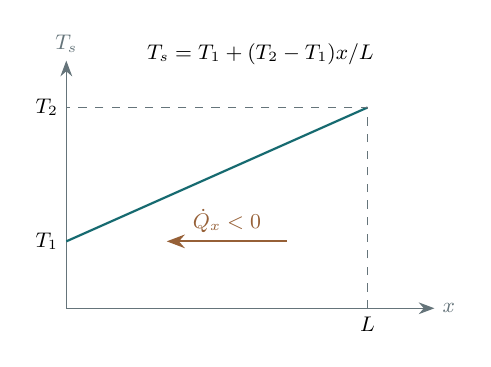
\begin{tikzpicture}[scale=.85,transform shape]

\draw[axis] (0,0)--(5.5,0) node[right] {$x$};
\draw[axis] (0,0)--(0,3.7) node[above] {$T_s$};
\draw[traj] (0,1)--(4.5,3);
\draw[guide] (4.5,0)--(4.5,3)--(0,3);
\node[left] at (0,1) {$T_1$};\node[left] at (0,3) {$T_2$};
\node[below] at (4.5,0) {$L$};
\draw[force] (3.3,1)--(1.5,1) node[midway,above] {$\dot Q_x<0$};
\node at (2.9,3.8) {$T_s=T_1+(T_2-T_1)x/L$};

\end{tikzpicture}
\figcaption{解图热试2.4A\quad 稳态温度梯度向右，热流由右向左。}
\end{minipage}\end{center}
解图热试2.4A中温度直线向右升高，热流箭头却向左，二者方向相反；稳态导热中各处温度随时间保持，同时热量持续从右端热源传向左端热源。

第（2）问把一次自由程向量记为$\boldsymbol\ell_j$。分子经过$M$段后
\[
\boldsymbol R=\sum_{j=1}^M\boldsymbol\ell_j,\qquad
\langle R^2\rangle
=\sum_j\langle\ell_j^2\rangle+
2\sum_{i<j}\langle\boldsymbol\ell_i\cdot\boldsymbol\ell_j\rangle.
\]
各段方向独立、各向同性，使不同段的交叉项在统计平均后为零，故
\[
\langle R^2\rangle=M\langle\ell^2\rangle.
\]
按给定指数分布，
\[
\langle\ell^2\rangle
=\int_0^\infty\ell^2\frac{e^{-\ell/\lambda}}{\lambda}\,\mathrm d\ell
=\lambda^2\int_0^\infty y^2e^{-y}\,\mathrm dy
=2\lambda^2.
\]
积分中的$\int_0^\infty y^2e^{-y}\mathrm dy$分部积分两次，依次化为$2\int_0^\infty ye^{-y}\mathrm dy=2\int_0^\infty e^{-y}\mathrm dy=2$；指数分布的长自由程尾部因此使二阶矩等于均值平方的2倍。长时间平均碰撞段数$M\simeq\bar vt/\lambda$，所以
\[
\boxed{R_{\rm rms}\simeq\sqrt{2\bar v\lambda t}}.
\]
\begin{center}\begin{minipage}{.98\linewidth}\centering
\begin{tikzpicture}[scale=.75,transform shape]

\draw[object] (0,0)--(.8,.45)--(.3,1.2)--(1.2,1.5)--(1.9,.9)--(1.5,.2)--(2.4,-.2)--(3,.6)--(2.8,1.3)--(3.6,1.7);
\fill (0,0) circle (1.7pt) node[below left] {$O$};
\fill (3.6,1.7) circle (1.7pt) node[above] {$P$};
\draw[motion] (0,0)--(3.6,1.7) node[midway,below right] {$\boldsymbol R$};
\draw[axis,<->] (.15,1.45)--(1.05,1.75) node[midway,above] {$\boldsymbol\ell_j$};
\node[right,align=left] at (4.4,1.2) {$\langle\boldsymbol\ell_i\cdot\boldsymbol\ell_j\rangle=0$\\[7pt]$\langle\ell^2\rangle=2\lambda^2$\\[7pt]$\langle R^2\rangle\simeq2\bar v\lambda t$};
\node at (3.5,-1) {折线路程与端到端位移不同};

\end{tikzpicture}
\figcaption{解图热试2.4B\quad 随机飞行的统计平均消去交叉项，单条轨迹仍会波动。}
\end{minipage}\end{center}
解图热试2.4B画同一模型中的折线轨迹与端到端位移；折线路程约为$\bar vt$，端到端位移只按$\sqrt t$增长。等体积、相同分子且质量比为2给$n_1=2n_2$，于是
\[
\frac{\lambda_1}{\lambda_2}=\frac12,\qquad
\frac{\bar v_1}{\bar v_2}=\sqrt{\frac{T_1}{T_2}},
\]
\[
\boxed{\frac{R_{1,\rm rms}}{R_{2,\rm rms}}
=\frac1{\sqrt2}\left(\frac{T_1}{T_2}\right)^{1/4}}.
\]
相同分子的平均速率为$\bar v=\sqrt{8k_BT/(\pi m)}$，硬球模型的平均自由程为$\lambda=1/(\sqrt2\pi d^2n)$，其中$d$为分子有效直径。用压强也能表达相同的密度信息：$p_1V=2\nu_2RT_1$、$p_2V=\nu_2RT_2$，所以$p_2/p_1=T_2/(2T_1)$。硬球自由程$\lambda=k_BT/(\sqrt2\pi d^2p)$给$R_{\rm rms}\propto T^{3/4}p^{-1/2}$，代入此压强比仍得上述四分之一次方结果。固体固定使两气区保持各自体积，压强由各自粒子数和温度确定。

这个比值描述许多轨迹的统计尺度。单条轨迹的交叉项随随机方向涨落，单个分子的位移也随之波动；取大量同条件轨迹的均方根后得到所求比值。

若定义扩散系数$D=\bar v\lambda/3$，则$\langle R^2\rangle=6Dt$，每一坐标的方差为$2Dt$。典型观察窗口既要满足$t\gg\lambda/\bar v$以积累许多次碰撞，也要使$R_{\rm rms}$小于到容器壁的距离，以保持所用自由空间随机飞行近似。这里统计的是位移平方的平均，路线长度则是许多自由程长度之和。

第（3）问中$\nu_1=2\nu_2$。固体初态有线性温度分布，等体积薄片的热容量均匀，所以其初始热能对应的平均温度为
\[
\bar T_{s0}=\frac1L\int_0^L T_s(x)\,\mathrm dx
=\frac{T_1+T_2}{2}.
\]
\begin{center}\begin{minipage}{.98\linewidth}\centering
\begin{tikzpicture}[scale=.85,transform shape]

\draw[guide,rounded corners] (-.3,-.4) rectangle (7.3,2.5);
\draw[object,fill=accent!8] (0,0) rectangle (2,2);
\draw[object,fill=muted!10] (2.5,0) rectangle (4.5,2);
\draw[object,fill=warm!8] (5,0) rectangle (7,2);
\node[align=center] at (1,1) {气区1\\$2K,\ T_1$};
\node[align=center] at (3.5,1) {固体\\$2K,\ \bar T_{s0}$};
\node[align=center] at (6,1) {气区2\\$K,\ T_2$};
\node[above] at (3.5,2.7) {$\bar T_{s0}=(T_1+T_2)/2$};
\node at (3.5,-1) {撤热源，整体绝热，最终各处同温 $T_f$};

\end{tikzpicture}
\figcaption{解图热试2.4C\quad 三个热容量权重与固体初始平均能量决定终温。}
\end{minipage}\end{center}
解图热试2.4C把三个热容量分别标为$2K,K,2K$，其中$K=\nu_2C_V$。撤热源后无外界热量、无体积功，能量守恒为
\[
2K(T_f-T_1)+K(T_f-T_2)
+\frac{2K}{L}\int_0^L[T_f-T_s(x)]\,\mathrm dx=0.
\]
固体每个厚度$\mathrm dx$的薄片具有热容量$2K\mathrm dx/L$，其最终能量变化为该热容量乘$T_f-T_s(x)$。把左右两气区与所有薄片的带符号能量变化相加，即得上式；刚性容器与固定隔体保持体积，所以所用气体热容量是定体热容量。积分得
\[
2(T_f-T_1)+(T_f-T_2)+2T_f-T_1-T_2=0,
\]
\[
\boxed{T_f=\frac{3T_1+2T_2}{5}}.
\]
该温度位于$T_1,T_2$之间。固体初始冷端会升温、热端会降温，整个固体的净吸放热取决于它与$T_f$的平均温差，每个薄片按自己的初温与最终温度之差计入代数热量。\begin{center}\begin{minipage}{.98\linewidth}\centering
\begin{tikzpicture}[scale=.8,transform shape]
\draw[axis] (0,0)--(10.7,0) node[right] {$x/L$};
\draw[axis] (0,0)--(0,3.2) node[above] {$(T_f-T_s)/\Delta T$};
\node[above] at (5,3.5) {冷端部分最终升温，热端部分最终降温};
\draw[traj] plot coordinates {(0.000000000,3.000000000) (0.083333333,2.975000000) (0.166666667,2.950000000) (0.250000000,2.925000000) (0.333333333,2.900000000) (0.416666667,2.875000000) (0.500000000,2.850000000) (0.583333333,2.825000000) (0.666666667,2.800000000) (0.750000000,2.775000000) (0.833333333,2.750000000) (0.916666667,2.725000000) (1.000000000,2.700000000) (1.083333333,2.675000000) (1.166666667,2.650000000) (1.250000000,2.625000000) (1.333333333,2.600000000) (1.416666667,2.575000000) (1.500000000,2.550000000) (1.583333333,2.525000000) (1.666666667,2.500000000) (1.750000000,2.475000000) (1.833333333,2.450000000) (1.916666667,2.425000000) (2.000000000,2.400000000) (2.083333333,2.375000000) (2.166666667,2.350000000) (2.250000000,2.325000000) (2.333333333,2.300000000) (2.416666667,2.275000000) (2.500000000,2.250000000) (2.583333333,2.225000000) (2.666666667,2.200000000) (2.750000000,2.175000000) (2.833333333,2.150000000) (2.916666667,2.125000000) (3.000000000,2.100000000) (3.083333333,2.075000000) (3.166666667,2.050000000) (3.250000000,2.025000000) (3.333333333,2.000000000) (3.416666667,1.975000000) (3.500000000,1.950000000) (3.583333333,1.925000000) (3.666666667,1.900000000) (3.750000000,1.875000000) (3.833333333,1.850000000) (3.916666667,1.825000000) (4.000000000,1.800000000) (4.083333333,1.775000000) (4.166666667,1.750000000) (4.250000000,1.725000000) (4.333333333,1.700000000) (4.416666667,1.675000000) (4.500000000,1.650000000) (4.583333333,1.625000000) (4.666666667,1.600000000) (4.750000000,1.575000000) (4.833333333,1.550000000) (4.916666667,1.525000000) (5.000000000,1.500000000) (5.083333333,1.475000000) (5.166666667,1.450000000) (5.250000000,1.425000000) (5.333333333,1.400000000) (5.416666667,1.375000000) (5.500000000,1.350000000) (5.583333333,1.325000000) (5.666666667,1.300000000) (5.750000000,1.275000000) (5.833333333,1.250000000) (5.916666667,1.225000000) (6.000000000,1.200000000) (6.083333333,1.175000000) (6.166666667,1.150000000) (6.250000000,1.125000000) (6.333333333,1.100000000) (6.416666667,1.075000000) (6.500000000,1.050000000) (6.583333333,1.025000000) (6.666666667,1.000000000) (6.750000000,0.975000000) (6.833333333,0.950000000) (6.916666667,0.925000000) (7.000000000,0.900000000) (7.083333333,0.875000000) (7.166666667,0.850000000) (7.250000000,0.825000000) (7.333333333,0.800000000) (7.416666667,0.775000000) (7.500000000,0.750000000) (7.583333333,0.725000000) (7.666666667,0.700000000) (7.750000000,0.675000000) (7.833333333,0.650000000) (7.916666667,0.625000000) (8.000000000,0.600000000) (8.083333333,0.575000000) (8.166666667,0.550000000) (8.250000000,0.525000000) (8.333333333,0.500000000) (8.416666667,0.475000000) (8.500000000,0.450000000) (8.583333333,0.425000000) (8.666666667,0.400000000) (8.750000000,0.375000000) (8.833333333,0.350000000) (8.916666667,0.325000000) (9.000000000,0.300000000) (9.083333333,0.275000000) (9.166666667,0.250000000) (9.250000000,0.225000000) (9.333333333,0.200000000) (9.416666667,0.175000000) (9.500000000,0.150000000) (9.583333333,0.125000000) (9.666666667,0.100000000) (9.750000000,0.075000000) (9.833333333,0.050000000) (9.916666667,0.025000000) (10.000000000,0.000000000)};
\node[below] at (0,-.12) {$0$};
\node[below] at (4,-.12) {$2/5$};
\node[below] at (10,-.12) {$1$};
\draw[guide] (0,1.8)--(10,1.8) node[right] {$0$};\node[left] at (0,0) {$-3/5$};\node[left] at (0,3) {$2/5$};\end{tikzpicture}
\figcaption{解图热试2.4D\quad 冷端部分最终升温，热端部分最终降温}
\end{minipage}\end{center}
图D用$\Delta T=T_2-T_1$表示固体局部的最终温差：$[T_f-T_s(x)]/\Delta T=2/5-x/L$。在$x=2L/5$处变号，冷端的$2L/5$长度最终升温，其余部分最终降温。固体净热量为$-K\Delta T/5$，区域1吸热$4K\Delta T/5$，区域2放热$3K\Delta T/5$，三者的代数和为零。温度场初态的不均匀与终态的共同温度在这个薄片积分中连续衔接。



\Needspace{8\baselineskip}

\pdfbookmark[3]{关键洞察}{q4-h5}

\subsection*{关键洞察}

位移的温度四分之一次方来自两层平方根：平均速率随$\sqrt T$变化，均方根位移又随平均速率的平方根变化。密度使区域1的平均自由程减半，进一步压低其位移尺度。撤热源后的终温与温度中点不同，因为区域1气体的热容量较大；固体虽初态线性分布，其能量仍与全部气体一起决定最终均温。

\Needspace{8\baselineskip}

\pdfbookmark[3]{易错点}{q4-h6}

\subsection*{易错点}

稳态表示各处温度随时间保持，不断的热流仍由两热源维持。自由程均值的平方$\lambda^2$与二阶矩$2\lambda^2$分别计算；统计平均使交叉项消失，单条轨迹仍保留随机涨落。实际路程随$t$增长，端到端位移的统计尺度随$\sqrt t$增长。固体能量按温度场积分，薄片的正、负温差都保留，最后得到整体的净吸放热。

\Needspace{8\baselineskip}

\pdfbookmark[3]{课堂讲解建议}{q4-h7}

\subsection*{课堂讲解建议}

先让学生在同一张图上画温度梯度和热流，指出热源维持的稳态与撤热源后的均温终态各是什么。随机飞行部分画两条段数相同而端点不同的折线，让学生分别报出路程和位移；再以两段向量展开$R^2$，解释统计平均消去交叉项的条件。

算二阶矩时让学生亲自做指数分布积分，随后用密度比与压强比两种写法求距离尺度比。撤去热源后把固体切成薄片，每片写出$\mathrm dC[T_f-T_s(x)]$，在图D标出变号位置。最后核算气区1吸热、气区2放热、固体净放热的比例，把三个代数热量相加为零，与总能量方程相连。

\Needspace{8\baselineskip}

\pdfbookmark[3]{变式训练}{q4-h8}

\subsection*{变式训练}

\begin{enumerate}
\Needspace{20\baselineskip}
\item 两区仍等体积、同种分子，分子数比改为$q$，求均方根位移比。
\textbf{解：}变图热试2.4V1中$n_1/n_2=q$，相同硬球分子的平均自由程比为$1/q$。温度决定平均速率，$\bar v_1/\bar v_2=(T_1/T_2)^{1/2}$。在同一观察时间内，$R_{\rm rms}^2=2\bar v\lambda t$，因此$R_{1,\rm rms}/R_{2,\rm rms}=q^{-1/2}(T_1/T_2)^{1/4}$。较大的粒子数密度缩短自由程，较高温度增加热速；两个效应在乘积$\bar v\lambda$中分别计入，$q=2$恢复本题。
\begin{center}\begin{minipage}{.98\linewidth}\centering
\begin{tikzpicture}[scale=.8,transform shape]
\draw[axis] (0,0)--(10.7,0) node[right] {$q=n_1/n_2$};
\draw[axis] (0,0)--(0,3.2) node[above] {$R_1/R_2$};
\node[above] at (5,3.5) {$T_2=2T_1$时位移尺度随粒子数比变化};
\draw[traj] plot coordinates {(0.000000000,2.854097076) (0.083333333,2.774326072) (0.166666667,2.700890420) (0.250000000,2.632993623) (0.333333333,2.569972676) (0.416666667,2.511270613) (0.500000000,2.456415654) (0.583333333,2.405005154) (0.666666667,2.356693097) (0.750000000,2.311180256) (0.833333333,2.268206356) (0.916666667,2.227543791) (1.000000000,2.188992532) (1.083333333,2.152375976) (1.166666667,2.117537533) (1.250000000,2.084337800) (1.333333333,2.052652210) (1.416666667,2.022369063) (1.500000000,1.993387865) (1.583333333,1.965617921) (1.666666667,1.938977143) (1.750000000,1.913391027) (1.833333333,1.888791772) (1.916666667,1.865117529) (2.000000000,1.842311741) (2.083333333,1.820322577) (2.166666667,1.799102438) (2.250000000,1.778607519) (2.333333333,1.758797430) (2.416666667,1.739634863) (2.500000000,1.721085294) (2.583333333,1.703116723) (2.666666667,1.685699439) (2.750000000,1.668805819) (2.833333333,1.652410136) (2.916666667,1.636488401) (3.000000000,1.621018210) (3.083333333,1.605978618) (3.166666667,1.591350010) (3.250000000,1.577114005) (3.333333333,1.563253350) (3.416666667,1.549751834) (3.500000000,1.536594212) (3.583333333,1.523766129) (3.666666667,1.511254055) (3.750000000,1.499045224) (3.833333333,1.487127583) (3.916666667,1.475489737) (4.000000000,1.464120907) (4.083333333,1.453010886) (4.166666667,1.442150001) (4.250000000,1.431529078) (4.333333333,1.421139409) (4.416666667,1.410972722) (4.500000000,1.401021152) (4.583333333,1.391277221) (4.666666667,1.381733805) (4.750000000,1.372384122) (4.833333333,1.363221703) (4.916666667,1.354240380) (5.000000000,1.345434264) (5.083333333,1.336797733) (5.166666667,1.328325412) (5.250000000,1.320012163) (5.333333333,1.311853069) (5.416666667,1.303843425) (5.500000000,1.295978723) (5.583333333,1.288254643) (5.666666667,1.280667044) (5.750000000,1.273211954) (5.833333333,1.265885561) (5.916666667,1.258684203) (6.000000000,1.251604364) (6.083333333,1.244642665) (6.166666667,1.237795856) (6.250000000,1.231060811) (6.333333333,1.224434522) (6.416666667,1.217914094) (6.500000000,1.211496738) (6.583333333,1.205179766) (6.666666667,1.198960588) (6.750000000,1.192836707) (6.833333333,1.186805714) (6.916666667,1.180865283) (7.000000000,1.175013171) (7.083333333,1.169247211) (7.166666667,1.163565310) (7.250000000,1.157965444) (7.333333333,1.152445659) (7.416666667,1.147004064) (7.500000000,1.141638830) (7.583333333,1.136348188) (7.666666667,1.131130426) (7.750000000,1.125983884) (7.833333333,1.120906958) (7.916666667,1.115898093) (8.000000000,1.110955780) (8.083333333,1.106078560) (8.166666667,1.101265015) (8.250000000,1.096513772) (8.333333333,1.091823499) (8.416666667,1.087192903) (8.500000000,1.082620729) (8.583333333,1.078105759) (8.666666667,1.073646809) (8.750000000,1.069242731) (8.833333333,1.064892408) (8.916666667,1.060594756) (9.000000000,1.056348720) (9.083333333,1.052153276) (9.166666667,1.048007427) (9.250000000,1.043910203) (9.333333333,1.039860660) (9.416666667,1.035857882) (9.500000000,1.031900976) (9.583333333,1.027989070) (9.666666667,1.024121320) (9.750000000,1.020296901) (9.833333333,1.016515009) (9.916666667,1.012774862) (10.000000000,1.009075698)};
\node[below] at (0,-.12) {$0.5$};
\node[below] at (4.285714285714286,-.12) {$2$};
\node[below] at (10,-.12) {$4$};
\end{tikzpicture}
\figcaption{变图热试2.4V1\quad $T_2=2T_1$时位移尺度随粒子数比变化}
\end{minipage}\end{center}

\Needspace{20\baselineskip}
\item 把指数自由程改为每段长度固定为$\lambda$，方向仍独立各向同性，求位移尺度和两区距离比。
\textbf{解：}变图热试2.4V2的向量长度相同，各方向仍随机。每段二阶矩变为$\langle\ell^2\rangle=\lambda^2$，故$\langle R^2\rangle=M\lambda^2\simeq\bar v\lambda t$，$R_{\rm rms}\simeq\sqrt{\bar v\lambda t}$。与指数长度模型相比，同一$\bar v,\lambda,t$的位移小$1/\sqrt2$；两区同时使用该模型时公共系数相消，距离比仍为$q^{-1/2}(T_1/T_2)^{1/4}$。指数分布的较长尾部增加的是单区的位移方差。
\begin{center}\begin{minipage}{.98\linewidth}\centering
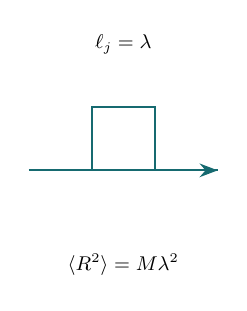
\begin{tikzpicture}[scale=.8,transform shape]
\draw[traj] (0,0)--(1,0)--(1,1)--(2,1)--(2,0)--(3,0);\draw[motion] (0,0)--(3,0);\node at (1.5,2) {$\ell_j=\lambda$};\node at (1.5,-1.5) {$\langle R^2\rangle=M\lambda^2$};
\end{tikzpicture}
\figcaption{变图热试2.4V2\quad 固定步长模型中位移方差由方向独立性相加}
\end{minipage}\end{center}

\Needspace{20\baselineskip}
\item 固体总热容量改为$bK$，两气区仍为$2K,K$，求最终温度并讨论$b$的极限。
\textbf{解：}变图热试2.4V3中固体初始平均温度仍为$(T_1+T_2)/2$。总能量给$(3+b)KT_f=2KT_1+KT_2+bK(T_1+T_2)/2$，所以$T_f=[(2+b/2)T_1+(1+b/2)T_2]/(3+b)$。$b=2$得到本题；$b\to0$时趋向两气区的加权平均$(2T_1+T_2)/3$，$b\to\infty$时趋向固体初始平均温度。图中横轴用固体热容量比，终温在这两极限之间连续变化。
\begin{center}\begin{minipage}{.98\linewidth}\centering
\begin{tikzpicture}[scale=.8,transform shape]
\draw[axis] (0,0)--(10.7,0) node[right] {$b=\nu_sC_s/K$};
\draw[axis] (0,0)--(0,3.2) node[above] {$T_f/T_1$};\foreach \y/\lab in {0/1.3,1.3/1.4,2.6/1.5}{\draw[thin] (0,\y)--(-.08,\y) node[left] {$\lab$};}
\node[above] at (5,3.5) {$T_2/T_1=2$时固体热容量对终温的影响};
\draw[traj] plot coordinates {(0.000000000,0.433333333) (0.083333333,0.480434783) (0.166666667,0.525531915) (0.250000000,0.568750000) (0.333333333,0.610204082) (0.416666667,0.650000000) (0.500000000,0.688235294) (0.583333333,0.725000000) (0.666666667,0.760377358) (0.750000000,0.794444444) (0.833333333,0.827272727) (0.916666667,0.858928571) (1.000000000,0.889473684) (1.083333333,0.918965517) (1.166666667,0.947457627) (1.250000000,0.975000000) (1.333333333,1.001639344) (1.416666667,1.027419355) (1.500000000,1.052380952) (1.583333333,1.076562500) (1.666666667,1.100000000) (1.750000000,1.122727273) (1.833333333,1.144776119) (1.916666667,1.166176471) (2.000000000,1.186956522) (2.083333333,1.207142857) (2.166666667,1.226760563) (2.250000000,1.245833333) (2.333333333,1.264383562) (2.416666667,1.282432432) (2.500000000,1.300000000) (2.583333333,1.317105263) (2.666666667,1.333766234) (2.750000000,1.350000000) (2.833333333,1.365822785) (2.916666667,1.381250000) (3.000000000,1.396296296) (3.083333333,1.410975610) (3.166666667,1.425301205) (3.250000000,1.439285714) (3.333333333,1.452941176) (3.416666667,1.466279070) (3.500000000,1.479310345) (3.583333333,1.492045455) (3.666666667,1.504494382) (3.750000000,1.516666667) (3.833333333,1.528571429) (3.916666667,1.540217391) (4.000000000,1.551612903) (4.083333333,1.562765957) (4.166666667,1.573684211) (4.250000000,1.584375000) (4.333333333,1.594845361) (4.416666667,1.605102041) (4.500000000,1.615151515) (4.583333333,1.625000000) (4.666666667,1.634653465) (4.750000000,1.644117647) (4.833333333,1.653398058) (4.916666667,1.662500000) (5.000000000,1.671428571) (5.083333333,1.680188679) (5.166666667,1.688785047) (5.250000000,1.697222222) (5.333333333,1.705504587) (5.416666667,1.713636364) (5.500000000,1.721621622) (5.583333333,1.729464286) (5.666666667,1.737168142) (5.750000000,1.744736842) (5.833333333,1.752173913) (5.916666667,1.759482759) (6.000000000,1.766666667) (6.083333333,1.773728814) (6.166666667,1.780672269) (6.250000000,1.787500000) (6.333333333,1.794214876) (6.416666667,1.800819672) (6.500000000,1.807317073) (6.583333333,1.813709677) (6.666666667,1.820000000) (6.750000000,1.826190476) (6.833333333,1.832283465) (6.916666667,1.838281250) (7.000000000,1.844186047) (7.083333333,1.850000000) (7.166666667,1.855725191) (7.250000000,1.861363636) (7.333333333,1.866917293) (7.416666667,1.872388060) (7.500000000,1.877777778) (7.583333333,1.883088235) (7.666666667,1.888321168) (7.750000000,1.893478261) (7.833333333,1.898561151) (7.916666667,1.903571429) (8.000000000,1.908510638) (8.083333333,1.913380282) (8.166666667,1.918181818) (8.250000000,1.922916667) (8.333333333,1.927586207) (8.416666667,1.932191781) (8.500000000,1.936734694) (8.583333333,1.941216216) (8.666666667,1.945637584) (8.750000000,1.950000000) (8.833333333,1.954304636) (8.916666667,1.958552632) (9.000000000,1.962745098) (9.083333333,1.966883117) (9.166666667,1.970967742) (9.250000000,1.975000000) (9.333333333,1.978980892) (9.416666667,1.982911392) (9.500000000,1.986792453) (9.583333333,1.990625000) (9.666666667,1.994409938) (9.750000000,1.998148148) (9.833333333,2.001840491) (9.916666667,2.005487805) (10.000000000,2.009090909)};
\node[below] at (0,-.12) {$0$};
\node[below] at (2.5,-.12) {$2$};
\node[below] at (10,-.12) {$8$};
\end{tikzpicture}
\figcaption{变图热试2.4V3\quad $T_2/T_1=2$时固体热容量对终温的影响}
\end{minipage}\end{center}

\Needspace{20\baselineskip}
\item 导热系数改为已知函数$k(T)>0$，截面积恒定，写稳态温度的隐式关系。
\textbf{解：}变图热试2.4V4中稳态仍有$\dot Q_x=-Ak(T)\mathrm dT/\mathrm dx$为常量。两边积分得$\int_{T_1}^{T_s(x)}k(T)\mathrm dT=-(\dot Q_x/A)x$，用$x=L,T_s=T_2$消去热流，得到$\int_{T_1}^{T_s(x)}k(T)\mathrm dT=(x/L)\int_{T_1}^{T_2}k(T)\mathrm dT$。正的$k(T)$使左侧对温度严格递增，故每个位置有唯一温度。撤热源后的固体初能由这个温度场重新积分。
\begin{center}\begin{minipage}{.98\linewidth}\centering
\begin{tikzpicture}[scale=.8,transform shape]
\draw[axis] (0,0)--(6,0) node[right] {$x$};\draw[axis] (0,0)--(0,4) node[above] {$\int_{T_1}^{T_s}k(T)\mathrm dT$};\draw[traj] (0,0)--(5,3);\node[below] at (5,0) {$L$};\node at (3,-1.5) {热导积分对位置线性变化};
\end{tikzpicture}
\figcaption{变图热试2.4V4\quad 变导热系数时线性的是积分变量}
\end{minipage}\end{center}

\Needspace{20\baselineskip}
\item 取$k(T)=k_0T/T_*$，固体热容量仍均匀且总量$2K$，求温度场与最终温度。
\textbf{解：}变图热试2.4V5对上题积分，得$T_s(x)=\sqrt{T_1^2+(T_2^2-T_1^2)x/L}$。平均初温为$\bar T_s=2(T_2^3-T_1^3)/[3(T_2^2-T_1^2)]$，所以$T_f=(2T_1+T_2+2\bar T_s)/5$。例如$T_2=2T_1$时$\bar T_s=14T_1/9$，$T_f=64T_1/45\simeq1.422222T_1$，高于恒导热系数的$7T_1/5$。较热部分对应更大的导热系数，温度场因此高于端点间的直线，固体初能也较高。
\begin{center}\begin{minipage}{.98\linewidth}\centering
\begin{tikzpicture}[scale=.8,transform shape]
\draw[axis] (0,0)--(10.7,0) node[right] {$x/L$};
\draw[axis] (0,0)--(0,3.2) node[above] {$T_s/T_1$};\foreach \y/\lab in {0/1,1.4/1.5,2.8/2}{\draw[thin] (0,\y)--(-.08,\y) node[left] {$\lab$};}
\node[above] at (5,3.5) {$T_2/T_1=2$：实线$k\propto T$，虚线常导热系数};
\draw[traj] plot coordinates {(0.000000000,0.000000000) (0.083333333,0.034783942) (0.166666667,0.069146214) (0.250000000,0.103101789) (0.333333333,0.136664775) (0.416666667,0.169848481) (0.500000000,0.202665483) (0.583333333,0.235127674) (0.666666667,0.267246322) (0.750000000,0.299032107) (0.833333333,0.330495168) (0.916666667,0.361645141) (1.000000000,0.392491190) (1.083333333,0.423042041) (1.166666667,0.453306011) (1.250000000,0.483291032) (1.333333333,0.513004679) (1.416666667,0.542454188) (1.500000000,0.571646482) (1.583333333,0.600588184) (1.666666667,0.629285640) (1.750000000,0.657744930) (1.833333333,0.685971887) (1.916666667,0.713972111) (2.000000000,0.741750979) (2.083333333,0.769313660) (2.166666667,0.796665122) (2.250000000,0.823810150) (2.333333333,0.850753347) (2.416666667,0.877499150) (2.500000000,0.904051835) (2.583333333,0.930415526) (2.666666667,0.956594202) (2.750000000,0.982591704) (2.833333333,1.008411742) (2.916666667,1.034057903) (3.000000000,1.059533651) (3.083333333,1.084842339) (3.166666667,1.109987212) (3.250000000,1.134971410) (3.333333333,1.159797975) (3.416666667,1.184469852) (3.500000000,1.208989898) (3.583333333,1.233360881) (3.666666667,1.257585489) (3.750000000,1.281666326) (3.833333333,1.305605924) (3.916666667,1.329406737) (4.000000000,1.353071153) (4.083333333,1.376601489) (4.166666667,1.400000000) (4.250000000,1.423268876) (4.333333333,1.446410249) (4.416666667,1.469426191) (4.500000000,1.492318721) (4.583333333,1.515089802) (4.666666667,1.537741348) (4.750000000,1.560275221) (4.833333333,1.582693236) (4.916666667,1.604997162) (5.000000000,1.627188724) (5.083333333,1.649269603) (5.166666667,1.671241438) (5.250000000,1.693105830) (5.333333333,1.714864339) (5.416666667,1.736518489) (5.500000000,1.758069767) (5.583333333,1.779519625) (5.666666667,1.800869483) (5.750000000,1.822120725) (5.833333333,1.843274706) (5.916666667,1.864332750) (6.000000000,1.885296149) (6.083333333,1.906166168) (6.166666667,1.926944045) (6.250000000,1.947630988) (6.333333333,1.968228182) (6.416666667,1.988736785) (6.500000000,2.009157930) (6.583333333,2.029492727) (6.666666667,2.049742261) (6.750000000,2.069907597) (6.833333333,2.089989775) (6.916666667,2.109989817) (7.000000000,2.129908721) (7.083333333,2.149747468) (7.166666667,2.169507018) (7.250000000,2.189188311) (7.333333333,2.208792270) (7.416666667,2.228319799) (7.500000000,2.247771786) (7.583333333,2.267149100) (7.666666667,2.286452595) (7.750000000,2.305683108) (7.833333333,2.324841461) (7.916666667,2.343928460) (8.000000000,2.362944896) (8.083333333,2.381891547) (8.166666667,2.400769174) (8.250000000,2.419578527) (8.333333333,2.438320341) (8.416666667,2.456995340) (8.500000000,2.475604231) (8.583333333,2.494147712) (8.666666667,2.512626469) (8.750000000,2.531041174) (8.833333333,2.549392489) (8.916666667,2.567681064) (9.000000000,2.585907537) (9.083333333,2.604072538) (9.166666667,2.622176685) (9.250000000,2.640220584) (9.333333333,2.658204833) (9.416666667,2.676130020) (9.500000000,2.693996724) (9.583333333,2.711805512) (9.666666667,2.729556944) (9.750000000,2.747251572) (9.833333333,2.764889936) (9.916666667,2.782472570) (10.000000000,2.800000000)};
\draw[dashed,thick,color=warm] plot coordinates {(0.000000000,0.000000000) (0.083333333,0.023333333) (0.166666667,0.046666667) (0.250000000,0.070000000) (0.333333333,0.093333333) (0.416666667,0.116666667) (0.500000000,0.140000000) (0.583333333,0.163333333) (0.666666667,0.186666667) (0.750000000,0.210000000) (0.833333333,0.233333333) (0.916666667,0.256666667) (1.000000000,0.280000000) (1.083333333,0.303333333) (1.166666667,0.326666667) (1.250000000,0.350000000) (1.333333333,0.373333333) (1.416666667,0.396666667) (1.500000000,0.420000000) (1.583333333,0.443333333) (1.666666667,0.466666667) (1.750000000,0.490000000) (1.833333333,0.513333333) (1.916666667,0.536666667) (2.000000000,0.560000000) (2.083333333,0.583333333) (2.166666667,0.606666667) (2.250000000,0.630000000) (2.333333333,0.653333333) (2.416666667,0.676666667) (2.500000000,0.700000000) (2.583333333,0.723333333) (2.666666667,0.746666667) (2.750000000,0.770000000) (2.833333333,0.793333333) (2.916666667,0.816666667) (3.000000000,0.840000000) (3.083333333,0.863333333) (3.166666667,0.886666667) (3.250000000,0.910000000) (3.333333333,0.933333333) (3.416666667,0.956666667) (3.500000000,0.980000000) (3.583333333,1.003333333) (3.666666667,1.026666667) (3.750000000,1.050000000) (3.833333333,1.073333333) (3.916666667,1.096666667) (4.000000000,1.120000000) (4.083333333,1.143333333) (4.166666667,1.166666667) (4.250000000,1.190000000) (4.333333333,1.213333333) (4.416666667,1.236666667) (4.500000000,1.260000000) (4.583333333,1.283333333) (4.666666667,1.306666667) (4.750000000,1.330000000) (4.833333333,1.353333333) (4.916666667,1.376666667) (5.000000000,1.400000000) (5.083333333,1.423333333) (5.166666667,1.446666667) (5.250000000,1.470000000) (5.333333333,1.493333333) (5.416666667,1.516666667) (5.500000000,1.540000000) (5.583333333,1.563333333) (5.666666667,1.586666667) (5.750000000,1.610000000) (5.833333333,1.633333333) (5.916666667,1.656666667) (6.000000000,1.680000000) (6.083333333,1.703333333) (6.166666667,1.726666667) (6.250000000,1.750000000) (6.333333333,1.773333333) (6.416666667,1.796666667) (6.500000000,1.820000000) (6.583333333,1.843333333) (6.666666667,1.866666667) (6.750000000,1.890000000) (6.833333333,1.913333333) (6.916666667,1.936666667) (7.000000000,1.960000000) (7.083333333,1.983333333) (7.166666667,2.006666667) (7.250000000,2.030000000) (7.333333333,2.053333333) (7.416666667,2.076666667) (7.500000000,2.100000000) (7.583333333,2.123333333) (7.666666667,2.146666667) (7.750000000,2.170000000) (7.833333333,2.193333333) (7.916666667,2.216666667) (8.000000000,2.240000000) (8.083333333,2.263333333) (8.166666667,2.286666667) (8.250000000,2.310000000) (8.333333333,2.333333333) (8.416666667,2.356666667) (8.500000000,2.380000000) (8.583333333,2.403333333) (8.666666667,2.426666667) (8.750000000,2.450000000) (8.833333333,2.473333333) (8.916666667,2.496666667) (9.000000000,2.520000000) (9.083333333,2.543333333) (9.166666667,2.566666667) (9.250000000,2.590000000) (9.333333333,2.613333333) (9.416666667,2.636666667) (9.500000000,2.660000000) (9.583333333,2.683333333) (9.666666667,2.706666667) (9.750000000,2.730000000) (9.833333333,2.753333333) (9.916666667,2.776666667) (10.000000000,2.800000000)};
\node[below] at (0,-.12) {$0$};
\node[below] at (5,-.12) {$1/2$};
\node[below] at (10,-.12) {$1$};
\end{tikzpicture}
\figcaption{变图热试2.4V5\quad $T_2/T_1=2$：实线$k\propto T$，虚线常导热系数}
\end{minipage}\end{center}

\Needspace{20\baselineskip}
\item 对本题求两气区与固体的净热量，并确定固体最终升温区域的长度。
\textbf{解：}变图热试2.4V6令$\Delta T=T_2-T_1>0$。最终温度为$T_1+2\Delta T/5$，气区1吸热$Q_1=4K\Delta T/5$，气区2的代数热量为$Q_2=-3K\Delta T/5$。固体净热量$Q_s=2K[T_f-(T_1+T_2)/2]=-K\Delta T/5$，三者相加为零。固体初温等于$T_f$的位置是$x=2L/5$，左侧薄片最终升温，右侧薄片最终降温；正、负局部能变的合计使固体净放热。
\begin{center}\begin{minipage}{.98\linewidth}\centering
\begin{tikzpicture}[scale=.8,transform shape]
\node[draw] (a) at (0,1) {气区1：$+4K\Delta T/5$};\node[draw] (s) at (5,1) {固体：$-K\Delta T/5$};\node[draw] (b) at (10,1) {气区2：$-3K\Delta T/5$};\draw[motion] (b)--(s);\draw[motion] (s)--(a);\node at (5,-1) {$Q_1+Q_s+Q_2=0$};
\end{tikzpicture}
\figcaption{变图热试2.4V6\quad 最终各部分能量变化相加为零}
\end{minipage}\end{center}

\Needspace{20\baselineskip}
\item 求撤热源后整个系统的熵增加，并说明其正号。
\textbf{解：}变图热试2.4V7令$r=T_2/T_1>1$、$f=T_f/T_1=(3+2r)/5$。两个气区的熵变为$2K\ln f+K\ln(f/r)$，固体熵变为$2K[\ln f-(r\ln r-r+1)/(r-1)]$，合计$\Delta S/K=5\ln f-\ln r-2(r\ln r-r+1)/(r-1)$。初态各部分的热容量加权平均温度就是$T_f$，对数的严格凹性给初态加权平均的$\ln T$小于$\ln T_f$，所以温差存在时$\Delta S>0$。能量守恒与不可逆熵增加同时成立。
\begin{center}\begin{minipage}{.98\linewidth}\centering
\begin{tikzpicture}[scale=.8,transform shape]
\draw[axis] (0,0)--(10.7,0) node[right] {$r=T_2/T_1$};
\draw[axis] (0,0)--(0,3.2) node[above] {$\Delta S/K$};
\node[above] at (5,3.5) {整体绝热平衡的不可逆熵增加};
\draw[traj] plot coordinates {(0.000500000,0.000000017) (0.083829167,0.000479913) (0.167158333,0.001880064) (0.250487500,0.004160132) (0.333816667,0.007281839) (0.417145833,0.011208845) (0.500475000,0.015906621) (0.583804167,0.021342346) (0.667133333,0.027484798) (0.750462500,0.034304260) (0.833791667,0.041772435) (0.917120833,0.049862360) (1.000450000,0.058548332) (1.083779167,0.067805836) (1.167108333,0.077611476) (1.250437500,0.087942917) (1.333766667,0.098778825) (1.417095833,0.110098816) (1.500425000,0.121883398) (1.583754167,0.134113932) (1.667083333,0.146772584) (1.750412500,0.159842281) (1.833741667,0.173306676) (1.917070833,0.187150110) (2.000400000,0.201357576) (2.083729167,0.215914690) (2.167058333,0.230807655) (2.250387500,0.246023239) (2.333716667,0.261548741) (2.417045833,0.277371973) (2.500375000,0.293481228) (2.583704167,0.309865263) (2.667033333,0.326513277) (2.750362500,0.343414887) (2.833691667,0.360560112) (2.917020833,0.377939355) (3.000350000,0.395543383) (3.083679167,0.413363315) (3.167008333,0.431390602) (3.250337500,0.449617017) (3.333666667,0.468034636) (3.416995833,0.486635829) (3.500325000,0.505413245) (3.583654167,0.524359804) (3.666983333,0.543468679) (3.750312500,0.562733292) (3.833641667,0.582147299) (3.916970833,0.601704585) (4.000300000,0.621399248) (4.083629167,0.641225598) (4.166958333,0.661178143) (4.250287500,0.681251583) (4.333616667,0.701440803) (4.416945833,0.721740864) (4.500275000,0.742146997) (4.583604167,0.762654597) (4.666933333,0.783259216) (4.750262500,0.803956558) (4.833591667,0.824742471) (4.916920833,0.845612942) (5.000250000,0.866564095) (5.083579167,0.887592181) (5.166908333,0.908693579) (5.250237500,0.929864785) (5.333566667,0.951102411) (5.416895833,0.972403181) (5.500225000,0.993763928) (5.583554167,1.015181586) (5.666883333,1.036653191) (5.750212500,1.058175872) (5.833541667,1.079746855) (5.916870833,1.101363452) (6.000200000,1.123023064) (6.083529167,1.144723173) (6.166858333,1.166461343) (6.250187500,1.188235216) (6.333516667,1.210042507) (6.416845833,1.231881007) (6.500175000,1.253748572) (6.583504167,1.275643131) (6.666833333,1.297562674) (6.750162500,1.319505257) (6.833491667,1.341468996) (6.916820833,1.363452065) (7.000150000,1.385452696) (7.083479167,1.407469176) (7.166808333,1.429499847) (7.250137500,1.451543100) (7.333466667,1.473597378) (7.416795833,1.495661170) (7.500125000,1.517733014) (7.583454167,1.539811492) (7.666783333,1.561895232) (7.750112500,1.583982901) (7.833441667,1.606073210) (7.916770833,1.628164907) (8.000100000,1.650256782) (8.083429167,1.672347661) (8.166758333,1.694436403) (8.250087500,1.716521908) (8.333416667,1.738603105) (8.416745833,1.760678957) (8.500075000,1.782748462) (8.583404167,1.804810645) (8.666733333,1.826864563) (8.750062500,1.848909301) (8.833391667,1.870943974) (8.916720833,1.892967723) (9.000050000,1.914979716) (9.083379167,1.936979146) (9.166708333,1.958965231) (9.250037500,1.980937215) (9.333366667,2.002894364) (9.416695833,2.024835967) (9.500025000,2.046761336) (9.583354167,2.068669802) (9.666683333,2.090560720) (9.750012500,2.112433464) (9.833341667,2.134287427) (9.916670833,2.156122021) (10.000000000,2.177936679)};
\node[below] at (0,-.12) {$1$};
\node[below] at (5,-.12) {$2$};
\node[below] at (10,-.12) {$3$};
\end{tikzpicture}
\figcaption{变图热试2.4V7\quad 整体绝热平衡的不可逆熵增加}
\end{minipage}\end{center}

\Needspace{20\baselineskip}
\item 在多次独立飞行的近似下，用三维高斯分布描述位移，求最概然位移与均方根位移的关系。
\textbf{解：}变图热试2.4V8中各坐标均值为零、方差为$R_{\rm rms}^2/3$。对半径为 $R$ 的球面上的各方向积分，径向密度为
\[
P(R)=4\pi R^2
 \left(\frac{3}{2\pi R_{\rm rms}^2}\right)^{3/2}
 \exp\left(-\frac{3R^2}{2R_{\rm rms}^2}\right).
\]令对数导数$2/R-3R/R_{\rm rms}^2=0$，得到$R_{\rm mode}=\sqrt{2/3}\,R_{\rm rms}$。均值为$\sqrt{8/(3\pi)}R_{\rm rms}$，又与均方根不同。图中的有限宽度展示单个分子的随机位移涨落，题目给出的比值指统计尺度。
\begin{center}\begin{minipage}{.98\linewidth}\centering
\begin{tikzpicture}[scale=.8,transform shape]
\draw[axis] (0,0)--(10.7,0) node[right] {$R/R_{\rm rms}$};
\draw[axis] (0,0)--(0,3.2) node[above] {$R_{\rm rms}P(R)$};
\node[above] at (5,3.5) {三维位移的径向概率密度具有有限宽度};
\draw[traj] plot coordinates {(0.000000000,0.000000000) (0.066666667,0.002993035) (0.133333333,0.011957185) (0.200000000,0.026847676) (0.266666667,0.047590194) (0.333333333,0.074081352) (0.400000000,0.106189328) (0.466666667,0.143754691) (0.533333333,0.186591381) (0.600000000,0.234487864) (0.666666667,0.287208433) (0.733333333,0.344494649) (0.800000000,0.406066922) (0.866666667,0.471626203) (0.933333333,0.540855785) (1.000000000,0.613423206) (1.066666667,0.688982215) (1.133333333,0.767174819) (1.200000000,0.847633370) (1.266666667,0.929982689) (1.333333333,1.013842210) (1.400000000,1.098828131) (1.466666667,1.184555550) (1.533333333,1.270640579) (1.600000000,1.356702416) (1.666666667,1.442365370) (1.733333333,1.527260810) (1.800000000,1.611029045) (1.866666667,1.693321110) (1.933333333,1.773800455) (2.000000000,1.852144514) (2.066666667,1.928046170) (2.133333333,2.001215088) (2.200000000,2.071378906) (2.266666667,2.138284311) (2.333333333,2.201697948) (2.400000000,2.261407208) (2.466666667,2.317220853) (2.533333333,2.368969508) (2.600000000,2.416505995) (2.666666667,2.459705537) (2.733333333,2.498465810) (2.800000000,2.532706864) (2.866666667,2.562370908) (2.933333333,2.587421971) (3.000000000,2.607845445) (3.066666667,2.623647505) (3.133333333,2.634854435) (3.200000000,2.641511848) (3.266666667,2.643683819) (3.333333333,2.641451945) (3.400000000,2.634914323) (3.466666667,2.624184475) (3.533333333,2.609390219) (3.600000000,2.590672499) (3.666666667,2.568184181) (3.733333333,2.542088827) (3.800000000,2.512559455) (3.866666667,2.479777294) (3.933333333,2.443930544) (4.000000000,2.405213145) (4.066666667,2.363823565) (4.133333333,2.319963620) (4.200000000,2.273837320) (4.266666667,2.225649762) (4.333333333,2.175606060) (4.400000000,2.123910330) (4.466666667,2.070764728) (4.533333333,2.016368547) (4.600000000,1.960917371) (4.666666667,1.904602296) (4.733333333,1.847609217) (4.800000000,1.790118178) (4.866666667,1.732302791) (4.933333333,1.674329724) (5.000000000,1.616358255) (5.066666667,1.558539890) (5.133333333,1.501018050) (5.200000000,1.443927822) (5.266666667,1.387395765) (5.333333333,1.331539782) (5.400000000,1.276469049) (5.466666667,1.222283987) (5.533333333,1.169076300) (5.600000000,1.116929049) (5.666666667,1.065916772) (5.733333333,1.016105647) (5.800000000,0.967553690) (5.866666667,0.920310987) (5.933333333,0.874419950) (6.000000000,0.829915610) (6.066666667,0.786825917) (6.133333333,0.745172077) (6.200000000,0.704968884) (6.266666667,0.666225084) (6.333333333,0.628943732) (6.400000000,0.593122564) (6.466666667,0.558754372) (6.533333333,0.525827373) (6.600000000,0.494325586) (6.666666667,0.464229195) (6.733333333,0.435514916) (6.800000000,0.408156348) (6.866666667,0.382124316) (6.933333333,0.357387208) (7.000000000,0.333911297) (7.066666667,0.311661045) (7.133333333,0.290599399) (7.200000000,0.270688073) (7.266666667,0.251887807) (7.333333333,0.234158619) (7.400000000,0.217460034) (7.466666667,0.201751301) (7.533333333,0.186991592) (7.600000000,0.173140184) (7.666666667,0.160156629) (7.733333333,0.148000906) (7.800000000,0.136633553) (7.866666667,0.126015796) (7.933333333,0.116109650) (8.000000000,0.106878018) (8.066666667,0.098284772) (8.133333333,0.090294821) (8.200000000,0.082874166) (8.266666667,0.075989954) (8.333333333,0.069610505) (8.400000000,0.063705347) (8.466666667,0.058245229) (8.533333333,0.053202136) (8.600000000,0.048549286) (8.666666667,0.044261132) (8.733333333,0.040313349) (8.800000000,0.036682820) (8.866666667,0.033347615) (8.933333333,0.030286971) (9.000000000,0.027481258) (9.066666667,0.024911954) (9.133333333,0.022561612) (9.200000000,0.020413819) (9.266666667,0.018453165) (9.333333333,0.016665202) (9.400000000,0.015036408) (9.466666667,0.013554141) (9.533333333,0.012206606) (9.600000000,0.010982810) (9.666666667,0.009872524) (9.733333333,0.008866244) (9.800000000,0.007955153) (9.866666667,0.007131079) (9.933333333,0.006386463) (10.000000000,0.005714320)};
\node[below] at (0,-.12) {$0$};
\node[below] at (3.265986323710904,-.12) {$\sqrt{2/3}$};
\node[below] at (4,-.12) {$1$};
\node[below] at (10,-.12) {$2.5$};
\end{tikzpicture}
\figcaption{变图热试2.4V8\quad 三维位移的径向概率密度具有有限宽度}
\end{minipage}\end{center}
\end{enumerate}

\Needspace{13\baselineskip}

\pdfbookmark[2]{第 5 题 光子气体的压强、绝热关系与辐射能流}{q5}

\section*{第 5 题\quad 光子气体的压强、绝热关系与辐射能流}\label{q:5}


黑体空腔的热辐射视为光子气体。频率为$\nu$的光子能量$\varepsilon=h\nu$、动量大小$p_\gamma=h\nu/c$；按频段记数密度$n_\nu$、能量密度$u_\nu=n_\nu h\nu$，总能量密度$u=\sum_\nu u_\nu$。光子静质量为零。热平衡时速度大小均为$c$，方向各向同性。
\begin{enumerate}
\item 先将壁面视为理想反射面，证明辐射压强$p=u/3$。
\item 对充分热化的黑体辐射，结合热力学第二定律说明$u$与壁材、腔体体积无关，只依赖温度，并导出$u=aT^4$。采用忽略表面与有限尺寸效应的宏观腔体近似。
\item 导出准静态可逆绝热过程中$p$与体积$V$的关系。
\item 求任意一光子的$x$方向速度分量分布$f(v_x)$。
\item 在壁上开一个不扰动内部平衡的小孔，证明单位孔面积的向外辐射功率$J=cu/4$，由此给出$J$随温度的规律。
\end{enumerate}
可用热力学恒等式
\[
\left(\frac{\partial U}{\partial V}\right)_T
=T\left(\frac{\partial p}{\partial T}\right)_V-p.
\]
空腔在求平衡态时允许吸收、发射以充分热化；反射面用于计算瞬时动量传递和理想绝热过程。


\begin{center}\begin{minipage}{.98\linewidth}\centering
\begin{tikzpicture}[scale=.9,transform shape]

\draw[object,fill=accent!4] (0,0) rectangle (6,3.6);
\draw[motion] (1,2.6)--(6,.8);
\draw[motion] (6,.8)--(3.77777778,0);
\draw[motion] (4.4,2.9)--(5.8,2.1);
\draw[motion] (1.1,.5)--(.15,1.8);
\draw[axis] (6,1.8)--(7.5,1.8) node[right] {$+\hat x$};
\node[align=center] at (2.2,3.1) {各向同性热辐射};
\node at (3,-1) {$\varepsilon=h\nu,\quad p_\gamma=\varepsilon/c$};
\node[below] at (3,-.2) {充分热化的宏观空腔};

\end{tikzpicture}
\figcaption{图热试2.5\quad 以腔壁法线定义x方向，光子方向各向同性。}
\end{minipage}\end{center}

\Needspace{8\baselineskip}

\pdfbookmark[3]{题型定位}{q5-h0}

\subsection*{题型定位}

以各向同性辐射的动量通量求压强，以能量通量求小孔辐射，再由充分热化的状态条件和热力学恒等式导出四次方律及可逆绝热线。五问沿同一物理链条展开：光子的反射动量、方向投影的统计平均、辐射的平衡状态变量、能量守恒与穿孔通量。

\Needspace{8\baselineskip}

\pdfbookmark[3]{知识点}{q5-h1}

\subsection*{知识点}

光子静质量为零，能量与动量满足$\varepsilon=cp_\gamma$。各向同性球面角概率为$\mathrm d\Omega/(4\pi)$，反射压强包含两次法向投影，小孔能流包含一次法向投影。充分热化允许光子被吸收、发射，平衡光子化学势为零；宏观辐射能量与体积成正比。热力学恒等式将$U=uV,p=u/3$联成$u\propto T^4$，可逆绝热则给$pV^{4/3}$不变。

\Needspace{8\baselineskip}

\pdfbookmark[3]{物理图像}{q5-h2}

\subsection*{物理图像}

解图热试2.5A中一束光先按法向速度到达壁面，再由反射交出两倍法向动量。图B将同温空腔与可输出功的活塞放在一起，说明热平衡压强的普适性。图C的绝热线向右下方延伸，膨胀同时降低温度与总辐射能。图D用速度球面上的球带求一个分量的分布，图E用小孔前的柱形体积求出射数通量。图F将两类角积分的权重分别画出，使$1/3$与$1/4$对应各自的面积。

\Needspace{8\baselineskip}

\pdfbookmark[3]{解题入口}{q5-h3}

\subsection*{解题入口}

先选一个频段和一个立体角，把单位面积到达壁面的能量写成$u_\nu c\cos\theta\mathrm d\Omega/(4\pi)$，再乘单位能量带来的反射法向动量$2\cos\theta/c$。求得压强后说明吸收、发射和宏观可加性所定义的黑体平衡，建立$u(T)$，再代入热力学恒等式。穿孔能流一问从速度分量密度出发，乘法向速度并只积分朝外的半轴。

\Needspace{8\baselineskip}

\pdfbookmark[3]{标准解法}{q5-h4}

\subsection*{标准解法}


图热试2.5取壁面外法线为$+\hat x$。光子静质量为零，动量大小为$\varepsilon/c$，反射受力直接按能量与动量的这一关系计算。
先看频段$\nu$、方向立体角$\mathrm d\Omega$内的一束光，能量密度为$u_\nu\mathrm d\Omega/(4\pi)$，与外法线夹角为$\theta$，只取指向壁面的半球$0\le\theta\le\pi/2$。
\begin{center}\begin{minipage}{.98\linewidth}\centering
\begin{tikzpicture}[scale=.85,transform shape]

\draw[object,line width=2pt] (3,-2.2)--(3,2.2);
\draw[motion] (-.2,1.8)--(3,0) node[pos=.36,above] {入射};
\draw[motion] (3,0)--(-.2,-1.8) node[pos=.7,below] {反射};
\draw[axis] (3,0)--(5.3,0) node[right] {$+\hat x$};
\draw[guide] (3,0)--(4.6,-.9);
\draw (3.85,0) arc[start angle=0,end angle=-29.36,radius=.85];
\node at (4.1,-.31) {$\theta$};
\draw[force] (3.1,.8)--(4.8,.8) node[midway,above] {$\Delta p_x=2\varepsilon\cos\theta/c$};
\node at (1,-2.6) {$\mathrm dJ=(u/4\pi)c\cos\theta\,\mathrm d\Omega$};

\end{tikzpicture}
\figcaption{解图热试2.5A\quad 碰撞通量与反射动量各含一次法向投影。}
\end{minipage}\end{center}
解图热试2.5A中单位面积、单位时间到达壁面的能量为
\[
\mathrm dJ_\nu=\frac{u_\nu}{4\pi}c\cos\theta\,\mathrm d\Omega.
\]
一次反射传给壁面的法向动量为$2(\varepsilon/c)\cos\theta$，所以该束光的压强贡献为
\[
\mathrm dp_\nu=\frac{2\cos\theta}{c}\,\mathrm dJ_\nu
=\frac{2u_\nu}{4\pi}\cos^2\theta\,\mathrm d\Omega.
\]
在光滑反射中，光子传给壁面的切向动量为零，法向动量在反射前后反向，壁面所获法向动量为正。一个$\cos\theta$来自光子在单位时间到达壁面的厚度$c\cos\theta\mathrm dt$，另一个来自单个光子的法向动量。对绕法线的方位角积分给$2\pi$，而朝壁面的极角只取$0$到$\pi/2$。用$\mathrm d\Omega=2\pi\sin\theta\,\mathrm d\theta$积分，
\[
p_\nu=\frac{2u_\nu}{4\pi}
\int_0^{\pi/2}\cos^2\theta\,2\pi\sin\theta\,\mathrm d\theta
=\frac{u_\nu}{3}.
\]
角积分$\int_0^{\pi/2}\cos^2\theta\sin\theta\mathrm d\theta$用$\mu=\cos\theta$换元后为$\int_0^1\mu^2\mathrm d\mu=1/3$。等价地，各向同性使三个方向的动量通量二阶矩相等，方向余弦平方之和为1，每一个方向贡献总能量密度的三分之一。对所有频段相加便得
\[
\boxed{p=\frac13u}.
\]

第（2）问先区分充分热化的黑体辐射与只反射、光子数被人为固定的非热化光场。黑体壁可以吸收、发射光子，平衡光子数随温度与体积调节；固定分子数气体还需指定的粒子密度，在这里由充分热化的平衡条件一同确定。
\begin{center}\begin{minipage}{.98\linewidth}\centering
\begin{tikzpicture}[scale=.75,transform shape]

\draw[object,fill=accent!5] (0,0) rectangle (2.8,2.4);
\draw[object,fill=warm!5] (5.5,0) rectangle (8.3,2.4);
\draw[object] (2.8,.8)--(5.5,.8);\draw[object] (2.8,1.6)--(5.5,1.6);
\draw[object,line width=2pt] (4.1,.8)--(4.1,1.6);
\node[align=center] at (1.4,1.2) {腔1\\壁材1，体积 $V_a$\\同温 $T$};
\node[align=center] at (6.9,1.2) {腔2\\壁材2，体积 $V_b$\\同温 $T$};
\node at (4.1,3.2) {反证假设：$u_1\ne u_2$};
\draw[force] (3,2)--(4,2);\draw[force] (5.2,2)--(4.4,2);
\node[above] at (3.4,2) {$p_1$};\node[above] at (4.9,2) {$p_2$};
\node at (4.1,-.8) {同一温度热库维持热化；活塞取功};

\end{tikzpicture}
\figcaption{解图热试2.5B\quad 同温壁材若能维持辐射压差，就可构造单温度取功矛盾。}
\end{minipage}\end{center}
解图热试2.5B的两个宏观空腔由同一温度热库维持。若仅因壁材不同就有不同的平衡辐射能量密度，由$p=u/3$也会有辐射压差，反射活塞受到相应的净推力。将两腔以小孔连通时，因方向分布相同，双向辐射通量各正比于所在腔的能量密度，净能量由较大$u$的一腔流向较小$u$的一腔。若同温下已有$u_1>u_2$，由温度变化的连续性，可把腔1温度略降至$T_c$、腔2略升至$T_h>T_c$，仍保持$u_1>u_2$，于是热量$Q$可从冷端自行传到热端。再令可逆热机从热端吸取同样的$Q$，向冷端放回$QT_c/T_h$，并输出$W=Q(1-T_c/T_h)>0$。热端恢复原状，光路和热机完成循环，唯一净结果是从冷端单一热库取热$W$并全部变功，违反开尔文表述。因此同温充分热化辐射的能量密度与壁材无关，辐射压强也相同。
体积方面，在忽略边界效应的宏观极限，充分热化辐射是均匀、可加的系统；将同温空腔分成或连成不同体积，不改变各局部的平衡状态。于是
\[
\boxed{u=u(T),\qquad U=u(T)V}.
\]
平衡条件还给出同一结论：光子数不守恒使化学势$\mu_\gamma=0$，均匀系统的欧拉关系为$U=TS-pV$；对欧拉关系直接微分有$\mathrm dU=T\mathrm dS+S\mathrm dT-p\mathrm dV-V\mathrm dp$，与$\mathrm dU=T\,\mathrm dS-p\,\mathrm dV$比较，得$S\,\mathrm dT=V\,\mathrm dp$。同温时$\mathrm dp=0$，压强由共同温度确定，改变宏观体积时保持相同。这里的$U$只计宏观腔内辐射能，腔壁能量另记。

这里的可加性指同温辐射系统的体积和能量同时放大时，能量密度保持不变；忽略表面与有限尺寸影响时，各局部处于同样的热平衡状态。光子数的吸收、发射使平衡态没有额外独立的数密度条件，能量的状态关系采用$U(S,V)$，光子的化学势为零。

将$U=u(T)V$与$p=u/3$代入题给恒等式：
\[
u=T\frac13\frac{\mathrm du}{\mathrm dT}-\frac13u,
\qquad
\frac{\mathrm du}{u}=4\frac{\mathrm dT}{T}.
\]
恒等式左侧的偏导在固定温度下取值，$u(T)$保持不变，所以$\partial U/\partial V=u$；右侧压强对温度的导数为$(1/3)\mathrm du/\mathrm dT$。整理后$T\mathrm du/\mathrm dT=4u$，从$(T_0,u_0)$积分有$\ln(u/u_0)=4\ln(T/T_0)$，正能量密度给正的比例常量$a=u_0/T_0^4$。积分得
\[
\boxed{u=aT^4,\qquad p=\frac a3T^4},
\]
其中$a$为与材料、体积无关的常量，其数值由微观统计或实验确定。

第（3）问在可逆准静态绝热过程中，
\[
\mathrm dU+p\,\mathrm dV=0.
\]
用$U=3pV$展开，
\[
3V\,\mathrm dp+3p\,\mathrm dV+p\,\mathrm dV=0,
\qquad
\frac{\mathrm dp}{p}+\frac43\frac{\mathrm dV}{V}=0.
\]
所以
\[
\boxed{pV^{4/3}=\text{常量}},
\qquad
\boxed{TV^{1/3}=\text{常量}}.
\]
\begin{center}\begin{minipage}{.98\linewidth}\centering
\begin{tikzpicture}[scale=.85,transform shape]

\draw[axis] (0,0)--(5.3,0) node[right] {$V$};
\draw[axis] (0,0)--(0,3.8) node[above] {$p$};
\draw[traj,domain=1:4.5,samples=70] plot (\x,{3.2/\x^1.3333333});
\draw[motion] (2,1.27)--(2.45,.969);
\node at (3.5,3.1) {$pV^{4/3}=\text{常量}$};
\node at (3.5,2.5) {$TV^{1/3}=\text{常量}$};
\node[below] at (2.8,.4) {膨胀降温};

\end{tikzpicture}
\figcaption{解图热试2.5C\quad 辐射可逆绝热膨胀曲线，指数由$U=3pV$决定。}
\end{minipage}\end{center}
进一步用$u=aT^4$写温度方程，$\mathrm dU=4aVT^3\mathrm dT+aT^4\mathrm dV$，第一定律化为$4aVT^3\mathrm dT+(4/3)aT^4\mathrm dV=0$，即$\mathrm dT/T+\mathrm dV/(3V)=0$。这给与压力式相同的温度绝热线。若体积从$V_i$变到$V_f$，总辐射能满足$U_f/U_i=(V_i/V_f)^{1/3}$，输出的体积功为$U_i-U_f$，热量为零。

解图热试2.5C的膨胀方向向右下，温度按$V^{-1/3}$下降。这里平衡光子数通过吸收、发射调节，指数$4/3$直接由辐射状态关系与能量守恒确定；固定物质的量气体的$C_p/C_V$则按粒子数固定的另一组状态约束定义。

第（4）问在速度空间中，所有端点都位于半径$c$的球面上且等概率。解图热试2.5D在$x$方向切取宽度$\mathrm dv_x$的球带。
\begin{center}\begin{minipage}{.98\linewidth}\centering
\begin{tikzpicture}[scale=.75,transform shape]

\draw[object] (0,0) circle (2.1);
\draw[guide] (0,0) ellipse (2.1 and .5);
\draw[axis] (-2.6,0)--(3.7,0) node[right] {$v_x$};
\draw[axis] (0,-2.5)--(0,2.6) node[above] {$v_z$};
\draw[traj] (.9,0) ellipse (.15 and 1.897);
\draw[traj] (1.2,0) ellipse (.15 and 1.723);
\draw[motion] (0,0)--(.9,1.897) node[midway,left] {$c$};
\draw[guide] (.9,-1.9)--(.9,-2.6)--(.5,-3.0);
\draw[guide] (1.2,-1.72)--(1.2,-2.6)--(2.1,-3);
\node[below] at (.5,-3) {$v_x$};
\node[below] at (2.3,-3) {$v_x+\mathrm dv_x$};
\node at (0,3.3) {$\mathrm dA_v=2\pi c\,\mathrm dv_x$};

\end{tikzpicture}
\figcaption{解图热试2.5D\quad 速度球面上等宽球带具有相同面积，分量分布为常量。}
\end{minipage}\end{center}
若$\mu=\cos\theta=v_x/c$，则球带面积为
\[
\mathrm dA_v=2\pi c^2\,\mathrm d\mu=2\pi c\,\mathrm dv_x.
\]
这个球带面积也可用圆周长解释：球带处的横截面半径为$\rho=\sqrt{c^2-v_x^2}$，圆周长为$2\pi\rho$；沿球面的带宽为$c\mathrm dv_x/\rho$，两者相乘后$\rho$约去，得到$2\pi c\mathrm dv_x$。因此等宽$\mathrm dv_x$的球带有相同面积，尽管它们的圆周长不同。除以球面总面积$4\pi c^2$即为概率：
\[
f(v_x)\,\mathrm dv_x=\frac{\mathrm dv_x}{2c}.
\]
因此
\[
\boxed{f(v_x)=
\begin{cases}
1/(2c),&-c\le v_x\le c,\\
0,&|v_x|>c.
\end{cases}}
\]
积分$\int_{-c}^c f(v_x)\,\mathrm dv_x=1$，且$\langle v_x^2\rangle=c^2/3$，与各向同性相符。

第（5）问，解图热试2.5E把孔外方向设为$v_x>0$。频段$\nu$中该速度分量区间内，每秒穿过单位孔面积的光子数是$n_\nu v_xf(v_x)\,\mathrm dv_x$，即该区间的数密度$n_\nu f(v_x)\mathrm dv_x$再乘法向速度$v_x$。因此
\[
J_\nu
=n_\nu h\nu\int_0^c v_x f(v_x)\,\mathrm dv_x
=u_\nu\int_0^c\frac{v_x}{2c}\,\mathrm dv_x
=\frac c4u_\nu.
\]
\begin{center}\begin{minipage}{.98\linewidth}\centering
\begin{tikzpicture}[scale=.85,transform shape]

\draw[object,line width=2pt] (0,-1.8)--(0,-.6);
\draw[object,line width=2pt] (0,.6)--(0,1.8);
\fill[accent!8] (-2.5,-.6) rectangle (0,.6);
\draw[guide] (-2.5,-.6)--(-2.5,.6);
\draw[motion] (-2, .3)--(1.3,.3) node[right] {$v_x>0$};
\draw[axis] (.2,-1)--(2,-1) node[right] {孔外};
\draw[axis,<->] (-2.5,-1)--(0,-1) node[midway,below] {$v_x\,\mathrm dt$};
\node[left] at (0,1.5) {腔内};
\node[right] at (.2,.9) {小孔};
\node at (0,-2.4) {$J=u\int_0^c v_xf(v_x)\,\mathrm dv_x=cu/4$};

\end{tikzpicture}
\figcaption{解图热试2.5E\quad 穿孔光子数按正的法向速度加权，积分只取出射半轴。}
\end{minipage}\end{center}
图E中速度区间内的光子在$\mathrm dt$内向外跨越厚度$v_x\mathrm dt$。单位孔面积前的这段体积内共有$n_\nu f(v_x)\mathrm dv_x\,v_x\mathrm dt$个光子，除以时间得到上述通量。只对$v_x>0$积分，既筛选出射方向，又按穿孔速度加权：
\[
\int_0^c v_x\frac{\mathrm dv_x}{2c}=\frac c4.
\]
这一系数在每个频段相同，故可以先求单频段再把能量密度相加。求和得
\[
\boxed{J=\frac c4u=\frac{ac}{4}T^4=\sigma T^4},
\qquad \sigma=\frac{ac}{4}.
\]
这里的$1/4$同时来自只取出射半空间和穿孔速度的投影加权。压强计算多一个法向动量因子，给$1/3$；两项角平均分别对应法向动量与穿孔能量。孔足够小且壁面继续维持热平衡，才能使用同一个内部$u(T)$计算连续辐射。\begin{center}\begin{minipage}{.98\linewidth}\centering
\begin{tikzpicture}[scale=.8,transform shape]
\draw[axis] (0,0)--(10.7,0) node[right] {$\mu=\cos\theta$};
\draw[axis] (0,0)--(0,3.2) node[above] {归一化角权重};
\node[above] at (5,3.5) {实线面积$p/u=1/3$，虚线面积$J/(cu)=1/4$};
\draw[traj] plot coordinates {(0.000000000,0.000000000) (0.083333333,0.000194444) (0.166666667,0.000777778) (0.250000000,0.001750000) (0.333333333,0.003111111) (0.416666667,0.004861111) (0.500000000,0.007000000) (0.583333333,0.009527778) (0.666666667,0.012444444) (0.750000000,0.015750000) (0.833333333,0.019444444) (0.916666667,0.023527778) (1.000000000,0.028000000) (1.083333333,0.032861111) (1.166666667,0.038111111) (1.250000000,0.043750000) (1.333333333,0.049777778) (1.416666667,0.056194444) (1.500000000,0.063000000) (1.583333333,0.070194444) (1.666666667,0.077777778) (1.750000000,0.085750000) (1.833333333,0.094111111) (1.916666667,0.102861111) (2.000000000,0.112000000) (2.083333333,0.121527778) (2.166666667,0.131444444) (2.250000000,0.141750000) (2.333333333,0.152444444) (2.416666667,0.163527778) (2.500000000,0.175000000) (2.583333333,0.186861111) (2.666666667,0.199111111) (2.750000000,0.211750000) (2.833333333,0.224777778) (2.916666667,0.238194444) (3.000000000,0.252000000) (3.083333333,0.266194444) (3.166666667,0.280777778) (3.250000000,0.295750000) (3.333333333,0.311111111) (3.416666667,0.326861111) (3.500000000,0.343000000) (3.583333333,0.359527778) (3.666666667,0.376444444) (3.750000000,0.393750000) (3.833333333,0.411444444) (3.916666667,0.429527778) (4.000000000,0.448000000) (4.083333333,0.466861111) (4.166666667,0.486111111) (4.250000000,0.505750000) (4.333333333,0.525777778) (4.416666667,0.546194444) (4.500000000,0.567000000) (4.583333333,0.588194444) (4.666666667,0.609777778) (4.750000000,0.631750000) (4.833333333,0.654111111) (4.916666667,0.676861111) (5.000000000,0.700000000) (5.083333333,0.723527778) (5.166666667,0.747444444) (5.250000000,0.771750000) (5.333333333,0.796444444) (5.416666667,0.821527778) (5.500000000,0.847000000) (5.583333333,0.872861111) (5.666666667,0.899111111) (5.750000000,0.925750000) (5.833333333,0.952777778) (5.916666667,0.980194444) (6.000000000,1.008000000) (6.083333333,1.036194444) (6.166666667,1.064777778) (6.250000000,1.093750000) (6.333333333,1.123111111) (6.416666667,1.152861111) (6.500000000,1.183000000) (6.583333333,1.213527778) (6.666666667,1.244444444) (6.750000000,1.275750000) (6.833333333,1.307444444) (6.916666667,1.339527778) (7.000000000,1.372000000) (7.083333333,1.404861111) (7.166666667,1.438111111) (7.250000000,1.471750000) (7.333333333,1.505777778) (7.416666667,1.540194444) (7.500000000,1.575000000) (7.583333333,1.610194444) (7.666666667,1.645777778) (7.750000000,1.681750000) (7.833333333,1.718111111) (7.916666667,1.754861111) (8.000000000,1.792000000) (8.083333333,1.829527778) (8.166666667,1.867444444) (8.250000000,1.905750000) (8.333333333,1.944444444) (8.416666667,1.983527778) (8.500000000,2.023000000) (8.583333333,2.062861111) (8.666666667,2.103111111) (8.750000000,2.143750000) (8.833333333,2.184777778) (8.916666667,2.226194444) (9.000000000,2.268000000) (9.083333333,2.310194444) (9.166666667,2.352777778) (9.250000000,2.395750000) (9.333333333,2.439111111) (9.416666667,2.482861111) (9.500000000,2.527000000) (9.583333333,2.571527778) (9.666666667,2.616444444) (9.750000000,2.661750000) (9.833333333,2.707444444) (9.916666667,2.753527778) (10.000000000,2.800000000)};
\draw[dashed,thick,color=warm] plot coordinates {(0.000000000,0.000000000) (0.083333333,0.011666667) (0.166666667,0.023333333) (0.250000000,0.035000000) (0.333333333,0.046666667) (0.416666667,0.058333333) (0.500000000,0.070000000) (0.583333333,0.081666667) (0.666666667,0.093333333) (0.750000000,0.105000000) (0.833333333,0.116666667) (0.916666667,0.128333333) (1.000000000,0.140000000) (1.083333333,0.151666667) (1.166666667,0.163333333) (1.250000000,0.175000000) (1.333333333,0.186666667) (1.416666667,0.198333333) (1.500000000,0.210000000) (1.583333333,0.221666667) (1.666666667,0.233333333) (1.750000000,0.245000000) (1.833333333,0.256666667) (1.916666667,0.268333333) (2.000000000,0.280000000) (2.083333333,0.291666667) (2.166666667,0.303333333) (2.250000000,0.315000000) (2.333333333,0.326666667) (2.416666667,0.338333333) (2.500000000,0.350000000) (2.583333333,0.361666667) (2.666666667,0.373333333) (2.750000000,0.385000000) (2.833333333,0.396666667) (2.916666667,0.408333333) (3.000000000,0.420000000) (3.083333333,0.431666667) (3.166666667,0.443333333) (3.250000000,0.455000000) (3.333333333,0.466666667) (3.416666667,0.478333333) (3.500000000,0.490000000) (3.583333333,0.501666667) (3.666666667,0.513333333) (3.750000000,0.525000000) (3.833333333,0.536666667) (3.916666667,0.548333333) (4.000000000,0.560000000) (4.083333333,0.571666667) (4.166666667,0.583333333) (4.250000000,0.595000000) (4.333333333,0.606666667) (4.416666667,0.618333333) (4.500000000,0.630000000) (4.583333333,0.641666667) (4.666666667,0.653333333) (4.750000000,0.665000000) (4.833333333,0.676666667) (4.916666667,0.688333333) (5.000000000,0.700000000) (5.083333333,0.711666667) (5.166666667,0.723333333) (5.250000000,0.735000000) (5.333333333,0.746666667) (5.416666667,0.758333333) (5.500000000,0.770000000) (5.583333333,0.781666667) (5.666666667,0.793333333) (5.750000000,0.805000000) (5.833333333,0.816666667) (5.916666667,0.828333333) (6.000000000,0.840000000) (6.083333333,0.851666667) (6.166666667,0.863333333) (6.250000000,0.875000000) (6.333333333,0.886666667) (6.416666667,0.898333333) (6.500000000,0.910000000) (6.583333333,0.921666667) (6.666666667,0.933333333) (6.750000000,0.945000000) (6.833333333,0.956666667) (6.916666667,0.968333333) (7.000000000,0.980000000) (7.083333333,0.991666667) (7.166666667,1.003333333) (7.250000000,1.015000000) (7.333333333,1.026666667) (7.416666667,1.038333333) (7.500000000,1.050000000) (7.583333333,1.061666667) (7.666666667,1.073333333) (7.750000000,1.085000000) (7.833333333,1.096666667) (7.916666667,1.108333333) (8.000000000,1.120000000) (8.083333333,1.131666667) (8.166666667,1.143333333) (8.250000000,1.155000000) (8.333333333,1.166666667) (8.416666667,1.178333333) (8.500000000,1.190000000) (8.583333333,1.201666667) (8.666666667,1.213333333) (8.750000000,1.225000000) (8.833333333,1.236666667) (8.916666667,1.248333333) (9.000000000,1.260000000) (9.083333333,1.271666667) (9.166666667,1.283333333) (9.250000000,1.295000000) (9.333333333,1.306666667) (9.416666667,1.318333333) (9.500000000,1.330000000) (9.583333333,1.341666667) (9.666666667,1.353333333) (9.750000000,1.365000000) (9.833333333,1.376666667) (9.916666667,1.388333333) (10.000000000,1.400000000)};
\node[below] at (0,-.12) {$0$};
\node[below] at (5,-.12) {$1/2$};
\node[below] at (10,-.12) {$1$};
\end{tikzpicture}
\figcaption{解图热试2.5F\quad 实线面积$p/u=1/3$，虚线面积$J/(cu)=1/4$}
\end{minipage}\end{center}
图F把法向方向余弦$\mu$从0到1的两项权重放在同一坐标中。压强的归一化积分是$\int_0^1\mu^2\mathrm d\mu=1/3$，孔流的归一化积分是$\int_0^1\mu\mathrm d\mu/2=1/4$，面积分别对应$p/u$和$J/(cu)$。因而$1/3$表示反射法向动量的平均，$1/4$表示出射能量的通量平均；两者共同使用内部各向同性的能量分布。



\Needspace{8\baselineskip}

\pdfbookmark[3]{关键洞察}{q5-h5}

\subsection*{关键洞察}

压力与能流分别统计法向动量和能量，二者的角权重不同。黑体辐射的四次方幂律由宏观状态关系确定，比例常量$a$由微观统计或实验确定；频谱细节在这一步尚未参与计算。光子数在充分热化中自行调节，辐射绝热指数$4/3$由$U=3pV$决定，与固定粒子数气体使用的比热比对应不同状态约束。

\Needspace{8\baselineskip}

\pdfbookmark[3]{易错点}{q5-h6}

\subsection*{易错点}

用$\varepsilon/c$计算光子动量，反射时法向分量反向、切向分量保持。壁面通量含$\cos\theta$，法向动量还再含一个$\cos\theta$，且积分区域只取朝壁面的半球。速度球面各向同性给$v_x\in[-c,c]$上的均匀密度，穿孔通量对正$v_x$再加一次速度权重。热力学状态公式用于充分热化的黑体辐射，固定光子数的任意孤立光场按各自能量与方向分布描述。

\Needspace{8\baselineskip}

\pdfbookmark[3]{课堂讲解建议}{q5-h7}

\subsection*{课堂讲解建议}

开头在图A让学生写一个反射光子的动量变化，区分法向翻转与切向保持。用两个不同倾角的光束比较“每秒到达多少”和“每个交出多少动量”，逐项得到两个余弦。随后把角积分和图F的面积联系起来，再与小孔能流的一次余弦比较。

热力学部分先问同温的普通气体还可选择什么状态参量，再说明黑体壁的吸收、发射使光子数随平衡调节。写出$U=TS-pV$并微分，让学生得到$S\mathrm dT=V\mathrm dp$，把同温压强保持相同与$p=u/3$相连，得到$u(T)$。最后在图D取球带推分量密度，在图E乘通量权重，完成$J=cu/4$和温度四次方律。

\Needspace{8\baselineskip}

\pdfbookmark[3]{变式训练}{q5-h8}

\subsection*{变式训练}

\begin{enumerate}
\Needspace{20\baselineskip}
\item 小孔面积为$A_h$，腔内温度由热库维持$T$，求总辐射功率及面积变化规律。
\textbf{解：}变图热试2.5V1在均匀内部辐射场中分别标出两个小孔。每单位面积向外的功率为$J=cu/4=\sigma T^4$，因此$P=A_h\sigma T^4$。保持内部温度时，小孔面积加倍，总功率也加倍，单位面积能流保持相同。热库不断补入同样的能量以维持稳态；所取孔面积足够小，使内部热化和均匀性在持续辐射中保持。功率的面积因子与温度四次方因子分别来自几何和辐射状态关系。
\begin{center}\begin{minipage}{.98\linewidth}\centering
\begin{tikzpicture}[scale=.8,transform shape]
\draw[very thick] (0,-1)--(0,3);\draw[line width=4pt,color=warm] (0,0)--(0,.4);\draw[line width=4pt,color=warm] (0,1.3)--(0,2.1);\draw[motion] (.2,.2)--(2,.2) node[right] {$A_h\sigma T^4$};\draw[motion] (.2,1.7)--(3,1.7) node[right] {$2A_h\sigma T^4$};\node[left] at (-.2,1) {$T$};
\end{tikzpicture}
\figcaption{变图热试2.5V1\quad 相同内部温度下，小孔总功率与面积成正比}
\end{minipage}\end{center}

\Needspace{20\baselineskip}
\item 黑体辐射准静态可逆绝热膨胀到8倍体积，求温度、压强和总能量的变化及输出功。
\textbf{解：}变图热试2.5V2令$r=V/V_i$，由$TV^{1/3}$不变得$T/T_i=r^{-1/3}$，$p/p_i=r^{-4/3}$，总能量$U/U_i=(u/u_i)r=r^{-1/3}$。当$r=8$时，温度降至$1/2$，压强降至$1/16$，总辐射能降至$1/2$。绝热过程$Q=0$，输出功$W=U_i-U_f=U_i/2$；光子能量随可逆膨胀减小，能量减少对应外部得到的机械功。
\begin{center}\begin{minipage}{.98\linewidth}\centering
\begin{tikzpicture}[scale=.8,transform shape]
\draw[axis] (0,0)--(10.7,0) node[right] {$V/V_i$};
\draw[axis] (0,0)--(0,3.2) node[above] {$T/T_i=U/U_i,\ p/p_i$};
\node[above] at (5,3.5) {实线为温度和总能量比，虚线为压强比};
\draw[traj] plot coordinates {(0.000000000,2.800000000) (0.083333333,2.747581223) (0.166666667,2.698879620) (0.250000000,2.653457132) (0.333333333,2.610945911) (0.416666667,2.571034360) (0.500000000,2.533456442) (0.583333333,2.497983384) (0.666666667,2.464417160) (0.750000000,2.432585331) (0.833333333,2.402336905) (0.916666667,2.373538996) (1.000000000,2.346074096) (1.083333333,2.319837841) (1.166666667,2.294737162) (1.250000000,2.270688745) (1.333333333,2.247617743) (1.416666667,2.225456688) (1.500000000,2.204144576) (1.583333333,2.183626082) (1.666666667,2.163850891) (1.750000000,2.144773127) (1.833333333,2.126350853) (1.916666667,2.108545644) (2.000000000,2.091322215) (2.083333333,2.074648094) (2.166666667,2.058493338) (2.250000000,2.042830281) (2.333333333,2.027633319) (2.416666667,2.012878708) (2.500000000,1.998544395) (2.583333333,1.984609868) (2.666666667,1.971056012) (2.750000000,1.957864993) (2.833333333,1.945020148) (2.916666667,1.932505885) (3.000000000,1.920307597) (3.083333333,1.908411581) (3.166666667,1.896804968) (3.250000000,1.885475658) (3.333333333,1.874412260) (3.416666667,1.863604042) (3.500000000,1.853040877) (3.583333333,1.842713205) (3.666666667,1.832611990) (3.750000000,1.822728683) (3.833333333,1.813055187) (3.916666667,1.803583830) (4.000000000,1.794307335) (4.083333333,1.785218792) (4.166666667,1.776311636) (4.250000000,1.767579626) (4.333333333,1.759016822) (4.416666667,1.750617569) (4.500000000,1.742376476) (4.583333333,1.734288406) (4.666666667,1.726348452) (4.750000000,1.718551933) (4.833333333,1.710894376) (4.916666667,1.703371502) (5.000000000,1.695979220) (5.083333333,1.688713614) (5.166666667,1.681570933) (5.250000000,1.674547584) (5.333333333,1.667640120) (5.416666667,1.660845236) (5.500000000,1.654159760) (5.583333333,1.647580646) (5.666666667,1.641104968) (5.750000000,1.634729912) (5.833333333,1.628452774) (5.916666667,1.622270953) (6.000000000,1.616181943) (6.083333333,1.610183333) (6.166666667,1.604272801) (6.250000000,1.598448108) (6.333333333,1.592707095) (6.416666667,1.587047682) (6.500000000,1.581467860) (6.583333333,1.575965691) (6.666666667,1.570539303) (6.750000000,1.565186888) (6.833333333,1.559906699) (6.916666667,1.554697048) (7.000000000,1.549556303) (7.083333333,1.544482883) (7.166666667,1.539475261) (7.250000000,1.534531957) (7.333333333,1.529651541) (7.416666667,1.524832625) (7.500000000,1.520073865) (7.583333333,1.515373960) (7.666666667,1.510731648) (7.750000000,1.506145704) (7.833333333,1.501614942) (7.916666667,1.497138210) (8.000000000,1.492714390) (8.083333333,1.488342398) (8.166666667,1.484021181) (8.250000000,1.479749714) (8.333333333,1.475527006) (8.416666667,1.471352089) (8.500000000,1.467224025) (8.583333333,1.463141902) (8.666666667,1.459104833) (8.750000000,1.455111954) (8.833333333,1.451162425) (8.916666667,1.447255431) (9.000000000,1.443390175) (9.083333333,1.439565883) (9.166666667,1.435781802) (9.250000000,1.432037197) (9.333333333,1.428331355) (9.416666667,1.424663576) (9.500000000,1.421033184) (9.583333333,1.417439515) (9.666666667,1.413881925) (9.750000000,1.410359785) (9.833333333,1.406872480) (9.916666667,1.403419413) (10.000000000,1.400000000)};
\draw[dashed,thick,color=warm] plot coordinates {(0.000000000,2.800000000) (0.083333333,2.596139738) (0.166666667,2.416907123) (0.250000000,2.258261389) (0.333333333,2.116983171) (0.416666667,1.990478214) (0.500000000,1.876634402) (0.583333333,1.773716012) (0.666666667,1.680284427) (0.750000000,1.595137922) (0.833333333,1.517265414) (0.916666667,1.445810556) (1.000000000,1.380043586) (1.083333333,1.319339056) (1.166666667,1.263158071) (1.250000000,1.211033997) (1.333333333,1.162560901) (1.416666667,1.117384111) (1.500000000,1.075192476) (1.583333333,1.035711975) (1.666666667,0.998700411) (1.750000000,0.963942979) (1.833333333,0.931248549) (1.916666667,0.900446538) (2.000000000,0.871384256) (2.083333333,0.843924648) (2.166666667,0.817944373) (2.250000000,0.793332148) (2.333333333,0.769987336) (2.416666667,0.747818715) (2.500000000,0.726743417) (2.583333333,0.706686006) (2.666666667,0.687577678) (2.750000000,0.669355553) (2.833333333,0.651962061) (2.916666667,0.635344401) (3.000000000,0.619454064) (3.083333333,0.604246411) (3.166666667,0.589680301) (3.250000000,0.575717758) (3.333333333,0.562323678) (3.416666667,0.549465565) (3.500000000,0.537113298) (3.583333333,0.525238918) (3.666666667,0.513816446) (3.750000000,0.502821706) (3.833333333,0.492232177) (3.916666667,0.482026859) (4.000000000,0.472186141) (4.083333333,0.462691695) (4.166666667,0.453526375) (4.250000000,0.444674120) (4.333333333,0.436119873) (4.416666667,0.427849508) (4.500000000,0.419849753) (4.583333333,0.412108136) (4.666666667,0.404612918) (4.750000000,0.397353048) (4.833333333,0.390318109) (4.916666667,0.383498274) (5.000000000,0.376884271) (5.083333333,0.370467338) (5.166666667,0.364239191) (5.250000000,0.358191997) (5.333333333,0.352318335) (5.416666667,0.346611180) (5.500000000,0.341063868) (5.583333333,0.335670081) (5.666666667,0.330423819) (5.750000000,0.325319385) (5.833333333,0.320351365) (5.916666667,0.315514610) (6.000000000,0.310804220) (6.083333333,0.306215531) (6.166666667,0.301744100) (6.250000000,0.297385694) (6.333333333,0.293136275) (6.416666667,0.288991991) (6.500000000,0.284949164) (6.583333333,0.281004284) (6.666666667,0.277153995) (6.750000000,0.273395090) (6.833333333,0.269724501) (6.916666667,0.266139295) (7.000000000,0.262636661) (7.083333333,0.259213910) (7.166666667,0.255868464) (7.250000000,0.252597853) (7.333333333,0.249399708) (7.416666667,0.246271756) (7.500000000,0.243211818) (7.583333333,0.240217801) (7.666666667,0.237287693) (7.750000000,0.234419565) (7.833333333,0.231611559) (7.916666667,0.228861892) (8.000000000,0.226168847) (8.083333333,0.223530773) (8.166666667,0.220946081) (8.250000000,0.218413242) (8.333333333,0.215930781) (8.416666667,0.213497280) (8.500000000,0.211111371) (8.583333333,0.208771734) (8.666666667,0.206477099) (8.750000000,0.204226239) (8.833333333,0.202017971) (8.916666667,0.199851153) (9.000000000,0.197724681) (9.083333333,0.195637493) (9.166666667,0.193588558) (9.250000000,0.191576883) (9.333333333,0.189601507) (9.416666667,0.187661503) (9.500000000,0.185755972) (9.583333333,0.183884045) (9.666666667,0.182044883) (9.750000000,0.180237672) (9.833333333,0.178461625) (9.916666667,0.176715981) (10.000000000,0.175000000)};
\node[below] at (0,-.12) {$1$};
\node[below] at (10,-.12) {$8$};
\end{tikzpicture}
\figcaption{变图热试2.5V2\quad 实线为温度和总能量比，虚线为压强比}
\end{minipage}\end{center}

\Needspace{20\baselineskip}
\item 各向同性单色光场只在理想反射壁中保存总能量$U$，求瞬时压强与小孔能流，并说明状态描述。
\textbf{解：}变图热试2.5V3的光子频率统一为$\nu_0$、方向各向同性，所以能量密度为$u=U/V$。反射动量的角平均仍给$p=u/3$，小孔能量通量仍给$J=cu/4$；这两个式子使用角分布和能量密度，与是否具有黑体频谱分开。纯反射保存了所指定的频率和光子数，描述该光场时直接保留这些参数；经过吸收、发射充分热化后，平衡辐射再按$u=aT^4$和温度确定的频谱描述。
\begin{center}\begin{minipage}{.98\linewidth}\centering
\begin{tikzpicture}[scale=.8,transform shape]
\draw[very thick] (0,0) rectangle (5,3);\draw[motion] (2.5,1.5)--(4,1.5);\draw[motion] (2.5,1.5)--(1,1.5);\draw[motion] (2.5,1.5)--(2.5,2.7);\draw[motion] (2.5,1.5)--(2.5,.3);\node at (2.5,-1) {固定频率$\nu_0$，方向各向同性};\node at (2.5,-2) {$p=U/(3V),\quad J=cU/(4V)$};
\end{tikzpicture}
\figcaption{变图热试2.5V3\quad 各向同性的非热化单色光场按给定能量和频率描述}
\end{minipage}\end{center}

\Needspace{20\baselineskip}
\item 由黑体辐射的欧拉关系求熵，并由熵不变导出绝热曲线。
\textbf{解：}变图热试2.5V4中充分热化辐射满足$U=TS-pV$。代入$U=aVT^4$和$p=aT^4/3$，得到$TS=4aVT^4/3$，故$S=4aVT^3/3$。可逆绝热过程沿图中的竖直等熵线，$VT^3$保持常量，因此$TV^{1/3}$保持常量，进一步给$pV^{4/3}$保持常量。指数来自辐射的平衡能量与熵关系；粒子数固定的普通气体则按另一组状态约束定义其摩尔比热比。
\begin{center}\begin{minipage}{.98\linewidth}\centering
\begin{tikzpicture}[scale=.8,transform shape]
\draw[axis] (0,0)--(5,0) node[right] {$S$};\draw[axis] (0,0)--(0,4) node[above] {$T$};\draw[motion] (3,3.5)--(3,1);\node[right] at (3,2.5) {$S=4aVT^3/3$};\node at (2.5,-1.5) {可逆绝热：$VT^3$保持常量};
\end{tikzpicture}
\figcaption{变图热试2.5V4\quad 等熵线给辐射的温度—体积绝热关系}
\end{minipage}\end{center}

\Needspace{20\baselineskip}
\item 把各向同性光场改为沿$\pm x$的两束反向单色光，每束能量密度为$u/2$，求垂直$x$壁面的压力和向$+x$小孔的能流。
\textbf{解：}变图热试2.5V5中向$+x$的光束每秒给单位面积送来$cu/2$的能量，反射传递的法向动量是入射能量的$2/c$倍，所以$x$壁压力为$u$。向$+x$小孔只有该束光出射，能流为$cu/2$。沿$y,z$方向没有动量通量，对应压力分量为零。总能量密度保持$u$，方向分布改变后压力张量和孔流随之改变；各向同性时才由三个方向的相同二阶矩得到$u/3$。
\begin{center}\begin{minipage}{.98\linewidth}\centering
\begin{tikzpicture}[scale=.8,transform shape]
\draw[very thick] (5,-1)--(5,2);\draw[motion] (1,.7)--(4.7,.7) node[midway,above] {$u/2,+x$};\draw[motion] (4.7,0)--(1,0) node[midway,below] {$u/2,-x$};\draw[force] (5,1.5)--(6.5,1.5) node[right] {$p_x=u$};\node at (3,-2) {向$+x$孔流：$J_x=cu/2$};
\end{tikzpicture}
\figcaption{变图热试2.5V5\quad 双向窄束光场的压力与能流由方向分布决定}
\end{minipage}\end{center}

\Needspace{20\baselineskip}
\item 各向同性辐射只接收与法线夹角$0\le\theta\le\theta_m$的出射光，求能流及该角锥对反射压强的贡献。
\textbf{解：}变图热试2.5V6对立体角积分。能流$J_m=(cu/2)\int_0^{\theta_m}\cos\theta\sin\theta\mathrm d\theta=(cu/4)\sin^2\theta_m$，占整个半球出射能流的比例为$\sin^2\theta_m$。同一角锥反射到壁面产生的压力为$p_m=u\int_0^{\theta_m}\cos^2\theta\sin\theta\mathrm d\theta=(u/3)(1-\cos^3\theta_m)$。图中两条归一化曲线在$\theta_m=\pi/2$均达到1，各自包含的方向投影权重保持不同。
\begin{center}\begin{minipage}{.98\linewidth}\centering
\begin{tikzpicture}[scale=.8,transform shape]
\draw[axis] (0,0)--(10.7,0) node[right] {$\theta_m$};
\draw[axis] (0,0)--(0,3.2) node[above] {$J_m/J,\ p_m/p$};
\node[above] at (5,3.5) {实线为能流比例，虚线为反射压力比例};
\draw[traj] plot coordinates {(0.000000000,0.000000000) (0.083333333,0.000479745) (0.166666667,0.001918651) (0.250000000,0.004315733) (0.333333333,0.007669346) (0.416666667,0.011977194) (0.500000000,0.017236323) (0.583333333,0.023443129) (0.666666667,0.030593359) (0.750000000,0.038682111) (0.833333333,0.047703843) (0.916666667,0.057652371) (1.000000000,0.068520877) (1.083333333,0.080301912) (1.166666667,0.092987403) (1.250000000,0.106568654) (1.333333333,0.121036359) (1.416666667,0.136380602) (1.500000000,0.152590866) (1.583333333,0.169656042) (1.666666667,0.187564435) (1.750000000,0.206303770) (1.833333333,0.225861205) (1.916666667,0.246223336) (2.000000000,0.267376208) (2.083333333,0.289305324) (2.166666667,0.311995654) (2.250000000,0.335431648) (2.333333333,0.359597244) (2.416666667,0.384475881) (2.500000000,0.410050506) (2.583333333,0.436303594) (2.666666667,0.463217151) (2.750000000,0.490772732) (2.833333333,0.518951453) (2.916666667,0.547733999) (3.000000000,0.577100647) (3.083333333,0.607031268) (3.166666667,0.637505351) (3.250000000,0.668502009) (3.333333333,0.700000000) (3.416666667,0.731977736) (3.500000000,0.764413300) (3.583333333,0.797284464) (3.666666667,0.830568700) (3.750000000,0.864243195) (3.833333333,0.898284871) (3.916666667,0.932670397) (4.000000000,0.967376208) (4.083333333,1.002378517) (4.166666667,1.037653337) (4.250000000,1.073176491) (4.333333333,1.108923633) (4.416666667,1.144870264) (4.500000000,1.180991749) (4.583333333,1.217263331) (4.666666667,1.253660151) (4.750000000,1.290157266) (4.833333333,1.326729661) (4.916666667,1.363352272) (5.000000000,1.400000000) (5.083333333,1.436647728) (5.166666667,1.473270339) (5.250000000,1.509842734) (5.333333333,1.546339849) (5.416666667,1.582736669) (5.500000000,1.619008251) (5.583333333,1.655129736) (5.666666667,1.691076367) (5.750000000,1.726823509) (5.833333333,1.762346663) (5.916666667,1.797621483) (6.000000000,1.832623792) (6.083333333,1.867329603) (6.166666667,1.901715129) (6.250000000,1.935756805) (6.333333333,1.969431300) (6.416666667,2.002715536) (6.500000000,2.035586700) (6.583333333,2.068022264) (6.666666667,2.100000000) (6.750000000,2.131497991) (6.833333333,2.162494649) (6.916666667,2.192968732) (7.000000000,2.222899353) (7.083333333,2.252266001) (7.166666667,2.281048547) (7.250000000,2.309227268) (7.333333333,2.336782849) (7.416666667,2.363696406) (7.500000000,2.389949494) (7.583333333,2.415524119) (7.666666667,2.440402756) (7.750000000,2.464568352) (7.833333333,2.488004346) (7.916666667,2.510694676) (8.000000000,2.532623792) (8.083333333,2.553776664) (8.166666667,2.574138795) (8.250000000,2.593696230) (8.333333333,2.612435565) (8.416666667,2.630343958) (8.500000000,2.647409134) (8.583333333,2.663619398) (8.666666667,2.678963641) (8.750000000,2.693431346) (8.833333333,2.707012597) (8.916666667,2.719698088) (9.000000000,2.731479123) (9.083333333,2.742347629) (9.166666667,2.752296157) (9.250000000,2.761317889) (9.333333333,2.769406641) (9.416666667,2.776556871) (9.500000000,2.782763677) (9.583333333,2.788022806) (9.666666667,2.792330654) (9.750000000,2.795684267) (9.833333333,2.798081349) (9.916666667,2.799520255) (10.000000000,2.800000000)};
\draw[dashed,thick,color=warm] plot coordinates {(0.000000000,0.000000000) (0.083333333,0.000719587) (0.166666667,0.002877484) (0.250000000,0.006471104) (0.333333333,0.011496139) (0.416666667,0.017946565) (0.500000000,0.025814655) (0.583333333,0.035090987) (0.666666667,0.045764458) (0.750000000,0.057822305) (0.833333333,0.071250118) (0.916666667,0.086031866) (1.000000000,0.102149918) (1.083333333,0.119585071) (1.166666667,0.138316579) (1.250000000,0.158322183) (1.333333333,0.179578142) (1.416666667,0.202059275) (1.500000000,0.225738991) (1.583333333,0.250589333) (1.666666667,0.276581018) (1.750000000,0.303683482) (1.833333333,0.331864923) (1.916666667,0.361092352) (2.000000000,0.391331639) (2.083333333,0.422547565) (2.166666667,0.454703873) (2.250000000,0.487763326) (2.333333333,0.521687755) (2.416666667,0.556438123) (2.500000000,0.591974579) (2.583333333,0.628256519) (2.666666667,0.665242643) (2.750000000,0.702891020) (2.833333333,0.741159148) (2.916666667,0.780004017) (3.000000000,0.819382174) (3.083333333,0.859249783) (3.166666667,0.899562696) (3.250000000,0.940276514) (3.333333333,0.981346652) (3.416666667,1.022728407) (3.500000000,1.064377022) (3.583333333,1.106247753) (3.666666667,1.148295933) (3.750000000,1.190477040) (3.833333333,1.232746759) (3.916666667,1.275061049) (4.000000000,1.317376208) (4.083333333,1.359648933) (4.166666667,1.401836388) (4.250000000,1.443896261) (4.333333333,1.485786831) (4.416666667,1.527467022) (4.500000000,1.568896468) (4.583333333,1.610035567) (4.666666667,1.650845543) (4.750000000,1.691288495) (4.833333333,1.731327455) (4.916666667,1.770926441) (5.000000000,1.810050506) (5.083333333,1.848665791) (5.166666667,1.886739567) (5.250000000,1.924240286) (5.333333333,1.961137623) (5.416666667,1.997402517) (5.500000000,2.033007214) (5.583333333,2.067925301) (5.666666667,2.102131746) (5.750000000,2.135602928) (5.833333333,2.168316672) (5.916666667,2.200252274) (6.000000000,2.231390532) (6.083333333,2.261713766) (6.166666667,2.291205847) (6.250000000,2.319852207) (6.333333333,2.347639865) (6.416666667,2.374557436) (6.500000000,2.400595148) (6.583333333,2.425744845) (6.666666667,2.450000000) (6.750000000,2.473355718) (6.833333333,2.495808737) (6.916666667,2.517357427) (7.000000000,2.538001789) (7.083333333,2.557743447) (7.166666667,2.576585641) (7.250000000,2.594533217) (7.333333333,2.611592611) (7.416666667,2.627771837) (7.500000000,2.643080465) (7.583333333,2.657529603) (7.666666667,2.671131873) (7.750000000,2.683901385) (7.833333333,2.695853711) (7.916666667,2.707005851) (8.000000000,2.717376208) (8.083333333,2.726984544) (8.166666667,2.735851952) (8.250000000,2.744000812) (8.333333333,2.751454752) (8.416666667,2.758238607) (8.500000000,2.764378370) (8.583333333,2.769901151) (8.666666667,2.774835126) (8.750000000,2.779209487) (8.833333333,2.783054392) (8.916666667,2.786400911) (9.000000000,2.789280973) (9.083333333,2.791727310) (9.166666667,2.793773399) (9.250000000,2.795453405) (9.333333333,2.796802123) (9.416666667,2.797854916) (9.500000000,2.798647654) (9.583333333,2.799216654) (9.666666667,2.799598617) (9.750000000,2.799830565) (9.833333333,2.799949776) (9.916666667,2.799993720) (10.000000000,2.800000000)};
\node[below] at (0,-.12) {$0$};
\node[below] at (5,-.12) {$\pi/4$};
\node[below] at (10,-.12) {$\pi/2$};
\end{tikzpicture}
\figcaption{变图热试2.5V6\quad 实线为能流比例，虚线为反射压力比例}
\end{minipage}\end{center}

\Needspace{20\baselineskip}
\item 黑体辐射在热库维持温度$T$时等温膨胀，体积增加$\Delta V$，求热量、功、内能和熵的变化。
\textbf{解：}变图热试2.5V7的压强$p=aT^4/3$保持常量，所以$W=p\Delta V=aT^4\Delta V/3$。内部能量$U=aT^4V$随体积增加，$\Delta U=aT^4\Delta V$；第一定律给$Q=\Delta U+W=4aT^4\Delta V/3$。可逆等温熵增为$Q/T=4aT^3\Delta V/3$，与$S=4aVT^3/3$一致。腔壁吸收、发射使新增体积也具有温度$T$的平衡辐射，因而等温过程的能量密度保持相同。
\begin{center}\begin{minipage}{.98\linewidth}\centering
\begin{tikzpicture}[scale=.8,transform shape]
\draw[axis] (0,0)--(6,0) node[right] {$V$};\draw[axis] (0,0)--(0,4) node[above] {$p$};\fill[accent!10] (1,0) rectangle (5,2);\draw[motion] (1,2)--(5,2);\node[above] at (3,2) {$p=aT^4/3$};\draw[<->] (1,-.5)--(5,-.5) node[midway,below] {$\Delta V$};\node at (3,-2) {$Q=4W,\quad\Delta U=3W$};
\end{tikzpicture}
\figcaption{变图热试2.5V7\quad 辐射等温膨胀中的热量分为内能增加和体积功}
\end{minipage}\end{center}

\Needspace{20\baselineskip}
\item 固定体积$V$的空腔经小孔面积$A_h$向空旷外界冷却，壁面热容量忽略、热化足够快，求温度随时间的变化。
\textbf{解：}变图热试2.5V8令$U=aVT^4$，损失功率$P=A_hcu/4=A_hcU/(4V)$。能量方程为$\dot U=-A_hcU/(4V)$，故$U(t)=U_0e^{-A_hct/(4V)}$，温度$T(t)=T_0e^{-A_hct/(16V)}$。图中横坐标$s=A_hct/(4V)$，能量比为$e^{-s}$，温度比为$e^{-s/4}$。热化时间远短于冷却时间使各时刻仍可用黑体状态关系；若壁面也储热，则把壁面内能一起加入左侧能量变化。
\begin{center}\begin{minipage}{.98\linewidth}\centering
\begin{tikzpicture}[scale=.8,transform shape]
\draw[axis] (0,0)--(10.7,0) node[right] {$s=A_hct/(4V)$};
\draw[axis] (0,0)--(0,3.2) node[above] {$U/U_0,\ T/T_0$};
\node[above] at (5,3.5) {实线为能量衰减，虚线为温度衰减};
\draw[traj] plot coordinates {(0.000000000,2.800000000) (0.083333333,2.708205081) (0.166666667,2.619419558) (0.250000000,2.533544771) (0.333333333,2.450485293) (0.416666667,2.370148830) (0.500000000,2.292446109) (0.583333333,2.217290786) (0.666666667,2.144599347) (0.750000000,2.074291018) (0.833333333,2.006287670) (0.916666667,1.940513736) (1.000000000,1.876896129) (1.083333333,1.815364155) (1.166666667,1.755849439) (1.250000000,1.698285847) (1.333333333,1.642609415) (1.416666667,1.588758273) (1.500000000,1.536672581) (1.583333333,1.486294462) (1.666666667,1.437567933) (1.750000000,1.390438851) (1.833333333,1.344854843) (1.916666667,1.300765257) (2.000000000,1.258121100) (2.083333333,1.216874984) (2.166666667,1.176981077) (2.250000000,1.138395047) (2.333333333,1.101074018) (2.416666667,1.064976518) (2.500000000,1.030062435) (2.583333333,0.996292972) (2.666666667,0.963630603) (2.750000000,0.932039034) (2.833333333,0.901483160) (2.916666667,0.871929027) (3.000000000,0.843343793) (3.083333333,0.815695695) (3.166666667,0.788954009) (3.250000000,0.763089020) (3.333333333,0.738071987) (3.416666667,0.713875109) (3.500000000,0.690471499) (3.583333333,0.667835151) (3.666666667,0.645940910) (3.750000000,0.624764448) (3.833333333,0.604282234) (3.916666667,0.584471505) (4.000000000,0.565310250) (4.083333333,0.546777176) (4.166666667,0.528851688) (4.250000000,0.511513867) (4.333333333,0.494744448) (4.416666667,0.478524796) (4.500000000,0.462836887) (4.583333333,0.447663289) (4.666666667,0.432987141) (4.750000000,0.418792134) (4.833333333,0.405062495) (4.916666667,0.391782966) (5.000000000,0.378938793) (5.083333333,0.366515702) (5.166666667,0.354499888) (5.250000000,0.342877999) (5.333333333,0.331637121) (5.416666667,0.320764763) (5.500000000,0.310248843) (5.583333333,0.300077677) (5.666666667,0.290239960) (5.750000000,0.280724762) (5.833333333,0.271521510) (5.916666667,0.262619976) (6.000000000,0.254010269) (6.083333333,0.245682822) (6.166666667,0.237628381) (6.250000000,0.229837996) (6.333333333,0.222303010) (6.416666667,0.215015051) (6.500000000,0.207966019) (6.583333333,0.201148082) (6.666666667,0.194553663) (6.750000000,0.188175436) (6.833333333,0.182006311) (6.916666667,0.176039434) (7.000000000,0.170268175) (7.083333333,0.164686121) (7.166666667,0.159287067) (7.250000000,0.154065016) (7.333333333,0.149014164) (7.416666667,0.144128899) (7.500000000,0.139403791) (7.583333333,0.134833592) (7.666666667,0.130413221) (7.750000000,0.126137767) (7.833333333,0.122002479) (7.916666667,0.118002762) (8.000000000,0.114134171) (8.083333333,0.110392408) (8.166666667,0.106773314) (8.250000000,0.103272869) (8.333333333,0.099887181) (8.416666667,0.096612490) (8.500000000,0.093445156) (8.583333333,0.090381659) (8.666666667,0.087418596) (8.750000000,0.084552674) (8.833333333,0.081780707) (8.916666667,0.079099617) (9.000000000,0.076506423) (9.083333333,0.073998244) (9.166666667,0.071572293) (9.250000000,0.069225874) (9.333333333,0.066956380) (9.416666667,0.064761289) (9.500000000,0.062638161) (9.583333333,0.060584638) (9.666666667,0.058598437) (9.750000000,0.056677352) (9.833333333,0.054819247) (9.916666667,0.053022059) (10.000000000,0.051283789)};
\draw[dashed,thick,color=warm] plot coordinates {(0.000000000,2.800000000) (0.083333333,2.776763619) (0.166666667,2.753720071) (0.250000000,2.730867754) (0.333333333,2.708205081) (0.416666667,2.685730480) (0.500000000,2.663442389) (0.583333333,2.641339260) (0.666666667,2.619419558) (0.750000000,2.597681762) (0.833333333,2.576124361) (0.916666667,2.554745859) (1.000000000,2.533544771) (1.083333333,2.512519624) (1.166666667,2.491668959) (1.250000000,2.470991327) (1.333333333,2.450485293) (1.416666667,2.430149433) (1.500000000,2.409982334) (1.583333333,2.389982596) (1.666666667,2.370148830) (1.750000000,2.350479658) (1.833333333,2.330973715) (1.916666667,2.311629647) (2.000000000,2.292446109) (2.083333333,2.273421769) (2.166666667,2.254555307) (2.250000000,2.235845413) (2.333333333,2.217290786) (2.416666667,2.198890138) (2.500000000,2.180642193) (2.583333333,2.162545681) (2.666666667,2.144599347) (2.750000000,2.126801945) (2.833333333,2.109152238) (2.916666667,2.091649001) (3.000000000,2.074291018) (3.083333333,2.057077084) (3.166666667,2.040006003) (3.250000000,2.023076590) (3.333333333,2.006287670) (3.416666667,1.989638075) (3.500000000,1.973126651) (3.583333333,1.956752251) (3.666666667,1.940513736) (3.750000000,1.924409981) (3.833333333,1.908439865) (3.916666667,1.892602281) (4.000000000,1.876896129) (4.083333333,1.861320317) (4.166666667,1.845873765) (4.250000000,1.830555398) (4.333333333,1.815364155) (4.416666667,1.800298979) (4.500000000,1.785358825) (4.583333333,1.770542654) (4.666666667,1.755849439) (4.750000000,1.741278158) (4.833333333,1.726827800) (4.916666667,1.712497362) (5.000000000,1.698285847) (5.083333333,1.684192270) (5.166666667,1.670215651) (5.250000000,1.656355020) (5.333333333,1.642609415) (5.416666667,1.628977880) (5.500000000,1.615459469) (5.583333333,1.602053244) (5.666666667,1.588758273) (5.750000000,1.575573633) (5.833333333,1.562498408) (5.916666667,1.549531691) (6.000000000,1.536672581) (6.083333333,1.523920185) (6.166666667,1.511273617) (6.250000000,1.498732000) (6.333333333,1.486294462) (6.416666667,1.473960139) (6.500000000,1.461728175) (6.583333333,1.449597721) (6.666666667,1.437567933) (6.750000000,1.425637978) (6.833333333,1.413807025) (6.916666667,1.402074255) (7.000000000,1.390438851) (7.083333333,1.378900005) (7.166666667,1.367456918) (7.250000000,1.356108793) (7.333333333,1.344854843) (7.416666667,1.333694286) (7.500000000,1.322626348) (7.583333333,1.311650259) (7.666666667,1.300765257) (7.750000000,1.289970587) (7.833333333,1.279265498) (7.916666667,1.268649248) (8.000000000,1.258121100) (8.083333333,1.247680321) (8.166666667,1.237326187) (8.250000000,1.227057979) (8.333333333,1.216874984) (8.416666667,1.206776494) (8.500000000,1.196761809) (8.583333333,1.186830233) (8.666666667,1.176981077) (8.750000000,1.167213655) (8.833333333,1.157527291) (8.916666667,1.147921310) (9.000000000,1.138395047) (9.083333333,1.128947840) (9.166666667,1.119579032) (9.250000000,1.110287973) (9.333333333,1.101074018) (9.416666667,1.091936527) (9.500000000,1.082874866) (9.583333333,1.073888404) (9.666666667,1.064976518) (9.750000000,1.056138590) (9.833333333,1.047374005) (9.916666667,1.038682155) (10.000000000,1.030062435)};
\node[below] at (0,-.12) {$0$};
\node[below] at (5,-.12) {$2$};
\node[below] at (10,-.12) {$4$};
\end{tikzpicture}
\figcaption{变图热试2.5V8\quad 实线为能量衰减，虚线为温度衰减}
\end{minipage}\end{center}
\end{enumerate}

\end{document}
